\mychapter{Probability}\label{ch1}

\section{Preliminaries}\label{ch1_sec1}

In this section we give some preliminaries on probabilistic terminology, independence, Gaussian random variables, and conditional expectation. The first and fourth of these are the most important for what follows. The reader with some familiarity with probability theory can safely skip this section.

\subsecbkm{ch1_sec1.1}{Probabilistic terminology}

Given a space $\Omega$ and a $\sigma$-field\index{À5@$\sigma$-field} (or $\sigma$-algebra) $\FC$ on it, a probability measure\index{Probability measure}, or just a probability, is a positive finite measure with total mass $1$. $(\Omega, \FC, \P)$ is called a probability space. Elements of $\FC$ are called events\index{Events}. Measurable functions from $\Omega$ to $\R$ are called random variables\index{Random variables} and are usually denoted $X$ or $Y$ instead of $f$ or $g$. The integral of $X$ with respect to $\P$\index{P1@$\P$} is called the expectation\index{Expectation} of $X$ or the expected value of $X$, and $\int X(\omega)\P(d\omega)$ is often written $\E X$\index{E1@$\E$}, while $\int_A X(\omega)\P(d\omega)$ is often written $\E[X; A]$. If an event occurs with probability one, one says ``almost surely''\index{Almost surely} instead of ``almost everywhere'' and writes a.s.\ What analysts call the characteristic function of a set probabilists call the indicator\index{Indicator} of the set; in this book we will use the notation $1_A$\index{$1_A$} for the function or random variable that is $1$ on $A$ and $0$ on the complement. The complement of $A$ is denoted $A^c$\index{AA1@$A^c$}.

If $A_n$ is a sequence of sets, $(A_n~\text{i.o.})$, read ``infinitely often,''\index{Infinitely often} is defined to be $\cap_{j=1}^{\infty} \cup_{n=j}^{\infty} A_n$. The following easy fact is called the Borel-Cantelli lemma\index{Borel-Cantelli lemma|(} or sometimes the first half of the Borel-Cantelli lemma.

\begin{proposition}\label{prop:ch1_1.1}
If $\sum_{n=1}^{\infty} \P(A_n) < \infty$, then $\P(A_n~\textnormal{i.o.}) = 0$.
\end{proposition}

\begin{proof}
Note $\P(A_n~\text{i.o.}) = \lim_{j\to\infty} \P(\cup_{n=j}^{\infty} A_n)$. If $\sum_{n=1}^{\infty} \P(A_n) < \infty$, then $\P(\cup_{n=j}^{\infty} A_n) \leq \sum_{n=j}^{\infty} \P(A_n) \to 0$ as $j \to \infty$.
\end{proof}

\index{Borel-Cantelli lemma|)}

Chebyshev's inequality\index{Chebyshev's inequality} is the following inequality.

\begin{proposition}\label{prop:ch1_1.2}
If $X \geq 0$, a.s., then
\[
    \P(X \geq a) \leq \E X/a.
\]
\end{proposition}

\begin{proof}
This follows from
\[
    \P(X \geq a) = \E[1_{(X\geq a)}] \leq \E[X/a; X \geq a] \leq \E X/a.
\]
\end{proof}

Jensen's inequality\index{Jensen's inequality} is the following.

\begin{proposition}\label{prop:ch1_1.3}
If $g$ is convex and $X$ and $g(X)$ are integrable, then
\[
    \E g(X) \geq g(\E X).
\]
\end{proposition}

\begin{proof}
If $g$ is convex, then $g$ lies above all its tangent lines. So for each $x_0$, there exists $c$ such that $g(X) \geq g(x_0) + c(X - x_0)$. Letting $x_0 = \E X$ and taking expectations on both sides, we obtain our result.
\end{proof}

The law\index{Law} or distribution\index{Distribution} of $X$ is the probability measure $\P_X$ on $\R$, given by
\begin{equation}\label{eq:ch1_1.1}
    \P_X(A) = \P(X \in A).
\end{equation}
Given any measure $\mu$ on $\R$ with total mass $1$, we can construct a random variable $X$ such that $\P_X = \mu$: let $\Omega = [0,1]$ and let $\P$ be Lebesgue measure on $[0,1]$. For $\omega \in [0,1]$, let
\begin{equation}\label{eq:ch1_1.2}
    X(\omega) = \inf\{t : \mu((-\infty,t]) \geq \omega\}.
\end{equation}
Then $\P_X((-\infty,a]) = \P(X \leq a) = \mu(-\infty,a]$ for each $a$, hence $\P_X = \mu$.

\begin{proposition}\label{prop:ch1_1.4}
If $f \geq 0$ or $f$ is bounded,
\[
    \E f(X) = \int f(x)\P_X(dx).
\]
\end{proposition}

\begin{proof}
If $f = 1_{(-\infty,a]}$, then
\begin{equation}\label{eq:ch1_1.3}
    \E f(X) = \P(X \leq a) = \P_X((-\infty,a]) = \int f(x)\P_X(dx).
\end{equation}
\mnewpage
By linearity we obtain our result for simple functions $f$. Taking limits then gives us our result for $f$ bounded or $f$ nonnegative.
\end{proof}

A random vector\index{Random vector} is just a measurable map from $\Omega$ to $\R^d$, and the definition of law and Proposition \ref{prop:ch1_1.4} extend to this case.

We will frequently use the following equality.

\begin{proposition}\label{prop:ch1_1.5}
If $X \geq 0$,
\begin{equation}\label{eq:ch1_1.4}
    \E X^p = \int_0^{\infty} p\lambda^{p-1}\P(X > \lambda)d\lambda.
\end{equation}
\end{proposition}

\begin{proof}
By Fubini's theorem, the right-hand side is equal to
\[
    \E\int_0^{\infty} p\lambda^{p-1}1_{(X>\lambda)}d\lambda = \E\int_0^X p\lambda^{p-1}d\lambda,
\]
which is equal to the left-hand side.
\end{proof}

\subsecbkm{ch1_sec1.2}{Independence}
\index{Independence}

Two events $A$, $B$ are independent if $\P(A \cap B) = \P(A)\P(B)$. This definition generalizes to $n$ events: $A_1,\ldots,A_n$ are independent if $\P(\cap_{i=1}^n A_i) = \prod_{i=1}^n \P(A_i)$. A $\sigma$-field $\FC$ is independent of a $\sigma$-field $\GC$ if each $A \in \FC$ is independent of each $B \in \GC$. The $\sigma$-field generated by $X$, denoted $\sigma(X)$, is the collection $\{(X \in A); A~\text{Borel}\}$. Two random variables are independent if the $\sigma$-fields generated by $X$, $Y$ are independent. The notion of an event and a random variable being independent, or a random variable and a $\sigma$-field being independent are defined in the obvious way. Note that if $X$ and $Y$ are independent and $f$ and $g$ are Borel measurable functions, then $f(X)$ and $g(Y)$ are independent.

An example of independent random variables is to let $\Omega = [0,1]^2$, $\P$ Lebesgue measure, $X$ a function of just the first variable, and $Y$ a function of just the second variable. In fact, it can be shown that independent random variables can always be represented by means of some suitable product space.

\begin{proposition}\label{prop:ch1_1.6}
If $X$, $Y$, and $XY$ are integrable and $X$ and $Y$ are independent, then $\E XY = (\E X)(\E Y)$.
\end{proposition}

\begin{proof}
If $X$ is of the form $\sum_{i=1}^I a_i1_{A_i}$, $Y$ is of the form $\sum_{j=1}^J b_j1_{B_j}$, and $X$ and $Y$ are independent, then by linearity and the definition of independence, $\E XY = (\E X)(\E Y)$. Approximating nonnegative $X$ and $Y$ by simple random variables of this form, we obtain our result by monotone convergence. The case of general $X$ and $Y$ then follows by linearity.
\end{proof}

The characteristic function\index{Characteristic function} of a random variable $X$ is the Fourier transform of its law: $\int e^{\im ux}\P_X(dx) = \E e^{\im uX}$ (we are using Proposition \ref{prop:ch1_1.4} here). If $X$ and $Y$ are independent, so are $e^{\im uX}$ and $e^{\im vY}$, and hence by Proposition \ref{prop:ch1_1.6}, $\E e^{\im(uX+vY)} = \E e^{\im uX}\E e^{\im vY}$. Thus when $X$ and $Y$ are independent, the joint characteristic function of $X$ and $Y$ factors into the product of the respective characteristic functions.

The converse also holds.

\begin{proposition}\label{prop:ch1_1.7}
If $\E e^{\im(uX+vY)} = \E e^{\im uX}\E e^{\im vY}$ for all $u$ and $v$, then $X$ and $Y$ are independent random variables.
\end{proposition}

\begin{proof}
Let $X'$ be a random variable with the same law as $X$, $Y'$ one with the same law as $Y$, and $X'$, $Y'$ independent. (We let $\Omega = [0,1]^2$, $\P$ Lebesgue measure, $X'$ a function of the first variable, and $Y'$ a function of the second variable defined as in \eqref{eq:ch1_1.2}.) Then $\E e^{\im(uX'+vY')} = \E e^{\im uX}\E e^{\im vY}$. Since $X,X'$ have the same law, they have the same characteristic function, and similarly for $Y,Y'$. Therefore $(X',Y')$ has the same joint characteristic function as $(X,Y)$. By the uniqueness of the Fourier transform, $(X',Y')$ has the same joint law as $(X,Y)$, which is easily seen to imply that $X$ and $Y$ are independent.
\end{proof}

The second half of the Borel-Cantelli lemma\index{Borel-Cantelli lemma} is the following assertion.

\begin{proposition}\label{prop:ch1_1.8}
If $A_n$ is a sequence of independent events and $\sum_1^\infty \P(A_n) \allowbreak= \infty$, then $\P(A_n~\textnormal{i.o.}) = 1$.
\end{proposition}

\begin{proof}
Note
\begin{align*}
    \P(\cup_{n=j}^N A_n) &= 1 - \P(\cup_{n=j}^N A_n^c) = 1 - \prod_{n=j}^N \P(A_n^c) \\
    &= 1 - \prod_{n=j}^N (1 - \P(A_n)) \geq 1 - \exp\Big(-\sum_{n=j}^N \P(A_n)\Big) \to 1
\end{align*}
as $N \to \infty$. So $\P(A_n~\text{i.o.}) = \lim_{j\to\infty}(\P(\cup_{n=j}^\infty A_n)) = 1$.
\end{proof}

\subsecbkm{ch1_sec1.3}{Gaussian random variables}

A mean zero, variance one, Gaussian\index{Gaussian} or normal\index{Normal|(} random variable is one where
\begin{equation}\label{eq:ch1_1.5}
    \P(X \in A) = \int_A \frac{1}{\sqrt{2\pi}}e^{-x^2/2}dx, \qquad A~\text{Borel}.
\end{equation}
We also describe such an $X$ as having an $\NC(0,1)$ distribution or law, read as a ``normal $0,1$'' law. It is routine to check that such an $X$ has mean or expectation $0$ and variance\index{Variance} $\E(X - \E X)^2 = 1$. It is standard (\cite[see][pp.~66-67]{Durrett1991}) that $\E e^{\im uX} = e^{-u^2/2}$. Such random variables exist by the construction in \eqref{eq:ch1_1.2}, with
\[
    \mu(dx) = (2\pi)^{-1/2}e^{-x^2/2}dx.
\]
$X$ has an $\NC(a,b^2)$ distribution if $X = bZ + a$ for some $Z$ having a $\NC(0,1)$ distribution.

A sequence of random variables $X_1,\ldots,X_n$ is said to be jointly normal\index{Jointly normal} if there exists a sequence of independent $\NC(0,1)$ random variables $Z_1,\ldots,Z_m$ and constants $b_{ij}$ and $a_i$ such that $X_i = \sum_{j=1}^m b_{ij}Z_j + a_i$, $i = 1,\ldots,n$. In matrix notation, $X = BZ + A$. For simplicity, in what follows let us take $A = 0$; the modifications for the general case are easy. The covariance\index{Covariance} of two random variables $X$ and $Y$ is defined to be $\E[(X-\E X)(Y-\E Y)]$. Since we are assuming our normal random variables are mean $0$, we can omit the centering at expectations. Given a sequence of mean $0$ random variables, we can talk about the covariance matrix, which is $\Cov(X) = \E XX^t$, where $X^t$ denotes the transpose of the vector $X$. In the above case, we see $\Cov(X) = \E[(BZ)(BZ)^t] = \E[BZZ^tB^t] = BB^t$, since $\E ZZ^t = I$, the identity.

Let us compute the joint characteristic function\index{Joint characteristic function} $\E e^{\im u^t X}$ of the vector $X$, where $u$ is an $n$-dimensional vector. First, if $v$ is an $m$-dimensional vector,
\[
    \E e^{\im v^t Z} = \E \prod_{j=1}^m e^{\im v_jZ_j} = \prod_{j=1}^m \E e^{\im v_jZ_j} = \prod_{j=1}^m e^{-v_j^2/2} = e^{-v^t v/2}
\]
using the independence of the $Z$s. So
\begin{equation}\label{eq:ch1_1.6}
    \E e^{\im u^t X} = \E e^{\im u^t BZ} = e^{-u^t BB^tu/2}.
\end{equation}
By taking $u = (0,\ldots,0,a,0,\ldots,0)$ to be a constant times the unit vector in the $j$th coordinate direction, we deduce that each of the $X$s is indeed normal. Taking $m = 2$, $a \in \R$, $B = \begin{pmatrix}b_1 & 0\\ 0 & b_2\end{pmatrix}$, and $u = (a,a)$, we see that the sum of an $\NC(0,b_1^2)$ and an independent $\NC(0,b_2^2)$ is an $\NC(0,b_1^2 + b_2^2)$. If $\Cov(X) = BB^t$ is a diagonal matrix, then the joint characteristic function of the $X$s factors, and so by Proposition \ref{prop:ch1_1.7}, the $X$s would in this case be independent.

If $X_n$ are normal\index{Normal|)} random variables converging in probability (i.e., in measure) to a random variable $X$, then $X$ is also normal. This follows since $\E e^{\im uX_n} \to \E e^{\im uX}$ by dominated convergence. The analogue for random vectors is also true.

Finally we will use the following estimate.

\begin{proposition}\label{prop:ch1_1.9}
If $Z$ is an $\NC(0,1)$ and $a > 1$,
\mpagebreak
\begin{equation}\label{eq:ch1_1.7}
    \P(Z \geq a) \leq e^{-a^2/2}.
\end{equation}
\end{proposition}

\begin{proof}
This follows from
\[
    \P(Z \geq a) \leq \int_a^\infty e^{-x^2/2}dx \leq \int_a^\infty (x/a)e^{-x^2/2}dx
\]
\end{proof}

\subsecbkm{ch1_sec1.4}{Conditional expectation}

A concept that will be used extensively in the rest of this book will be that of conditional expectation\index{Conditional expectation}.

\begin{definition}\label{def:ch1_1.10}
If $\FC \subseteq \GC$ are two $\sigma$-fields and $X$ is an integrable $\GC$ measurable random variable, the conditional expectation of $X$ given $\FC$, written $\E[X\mid \FC]$\index{E2@$\E[X\mid \FC]$} and read as ``the expectation (or expected value) of $X$ given $\FC$,'' is any $\FC$ measurable random variable $Y$ such that $\E[Y;A] = \E[X;A]$ for every $A \in \FC$.
\end{definition}

If $Y_1,Y_2$ are two $\FC$ measurable random variables with $\E[Y_1;A] = \E[Y_2;A]$ for all $A \in \FC$, then $Y_1 = Y_2$, a.s., or conditional expectation is unique up to a.s.\ equivalence.

In the case $X$ is already $\FC$ measurable, $\E[X\mid \FC] = X$. If $X$ is independent of $\FC$, $\E[X\mid \FC] = \E X$. Both of these facts follow immediately from the definition. For another example, which ties this definition with the one used in elementary probability courses, if $\{A_i\}$ is a finite collection of disjoint sets whose union is $\Omega$, $\P(A_i) > 0$ for all $i$, and $\FC$ is the $\sigma$-field generated by the $A_i$s, then
\begin{equation}\label{eq:ch1_1.8}
    \E[X\mid \FC] = \sum_i \frac{\E[X;A_i]}{\P(A_i)}1_{A_i}.
\end{equation}
This follows since the right-hand side is $\FC$ measurable and its expectation over any set $A_i$ is $\E[X;A_i]$.

It is easy to check that limit theorems such as monotone convergence and dominated convergence have conditional expectation versions, as do inequalities like Jensen's and Chebyshev's inequalities. Thus, for example, we have the following.

\begin{proposition}[Jensen's inequality\index{Jensen's inequality} for conditional expectations]\label{prop:ch1_1.11}
If $g$ is convex and $X$ and $g(X)$ are integrable,
\begin{equation}\label{eq:ch1_1.9}
    \E[g(X)\mid \FC] \geq g(\E[X\mid \FC]), \qquad \textnormal{a.s.}
\end{equation}
\end{proposition}

\mpagebreak

A key fact is the following.

\begin{proposition}\label{prop:ch1_1.12}
If $X$ and $XY$ are integrable and $Y$ is measurable with respect to $\FC$, then
\begin{equation}\label{eq:ch1_1.10}
    \E[XY\mid \FC] = Y\E[X\mid \FC].
\end{equation}
\end{proposition}

\begin{proof}
If $A \in \FC$, then for any $B \in \FC$,
\[
    \E\big[1_A\E[X\mid \FC];B\big] = \E\big[\E[X\mid \FC];A \cap B\big] = \E[X;A \cap B] = \E[1_AX;B].
\]
Since $1_A\E[X\mid \FC]$ is $\FC$ measurable, this shows that \eqref{eq:ch1_1.10} holds when $Y = 1_A$ and $A \in \FC$. Using linearity and taking limits shows that \eqref{eq:ch1_1.10} holds whenever $Y$ is $\FC$ measurable and $X$ and $XY$ are integrable.
\end{proof}

Two other equalities follow.

\begin{proposition}\label{prop:ch1_1.13}
If $\EC \subseteq \FC \subseteq \GC$, then
\begin{equation}\label{eq:ch1_1.11}
    \E\big[\E[X\mid \FC]\mid \EC\big] = \E[X\mid \EC] = \E\big[\E[X\mid \EC]\mid \FC\big].
\end{equation}
\end{proposition}

\begin{proof}
The right equality holds because $\E[X\mid \EC]$ is $\EC$ measurable, hence $\FC$ measurable. To show the left equality, let $A \in \EC$. Then since $A$ is also in $\FC$,
\[
    \E\big[\E[\E[X\mid \FC]\mid \EC];A\big] = \E\big[\E[X\mid \FC];A\big] = \E[X;A] = \E\big[\E[X\mid \EC];A\big].
\]
Since both sides are $\EC$ measurable, the equality follows.
\end{proof}

To show the existence of $\E[X\mid \FC]$, we proceed as follows.

\begin{proposition}\label{prop:ch1_1.14}
If $X$ is integrable, then $\E[X\mid \FC]$ exists.
\end{proposition}

\begin{proof}
Using linearity, we need only consider $X \geq 0$. Define a measure $\Q$ on $\FC$ by $\Q(A) = \E[X;A]$ for $A \in \FC$. This is trivially absolutely continuous with respect to $\P|_\FC$, the restriction of $\P$ to $\FC$. Let $\E[X\mid \FC]$ be the Radon-Nikodym derivative of $\Q$ with respect to $\P|_\FC$. The Radon-Nikodym derivative is $\FC$ measurable by construction and so provides the desired random variable.
\end{proof}

Equation \eqref{eq:ch1_1.10} shows that if $Y$ is $\FC$ measurable, then $\E\big[Y(X - \E[X\mid \FC])\big] = \E XY - \E\big[Y\E[X\mid \FC]\big] = 0$. So one way to view conditional expectation is that if $X \in L^2(\P)$, then $\E[X\mid \FC]$ is the projection\index{Projection} of $X$ onto the subspace of $L^2(\P)$ generated by the $\FC$ measurable functions, or the conditional expectation operator on $L^2(\P)$ is the projection operator onto this subspace. The conditional expectation operator on $L^1(\P)$ is then the (unique) extension of this projection operator.

\mpagebreak

When $\FC = \sigma(Y)$, one usually writes $\E[X\mid Y]$ for $\E[X\mid\FC]$. Notation that is commonly used (however, we will use it only very occasionally and only for heuristic purposes) is $\E[X\mid Y = y]$. The definition is as follows. If $A \in \sigma(Y)$, then $A = (Y \in B)$ for some Borel set $B$ by the definition of $\sigma(Y)$, or $1_A = 1_B(Y)$. By linearity and taking limits, if $Z$ is $\sigma(Y)$ measurable, $Z = f(Y)$ for some Borel measurable function $f$. Set $Z = \E[X\mid Y]$ and choose $f$ Borel measurable so that $Z = f(Y)$. Then $\E[X\mid Y = y]$ is defined to be $f(y)$.

\section{Brownian motion}\label{ch1_sec2}

In this section we construct Brownian motion\index{Brownian motion} and examine a few of its easiest properties. The reader who is not very familiar with probability should probably skip the subsection on the construction of Brownian motion for the first reading.

\subsecbkm{ch1_sec2.1}{Definitions}

Let $(\Omega, \FC, \P)$ be a probability space and let $\BC$ be the Borel $\sigma$-field on $[0,\infty)$. A stochastic process\index{Stochastic process}, denoted $X(t,\omega)$ or $X_t(\omega)$ or just $X_t$, is a map from $[0,\infty) \times \Omega$ to $\R$ that is measurable with respect to the product $\sigma$-field of $\BC$ and $\FC$.

\begin{definition}\label{def:ch1_2.1}
A stochastic process $X_t$ is a one-dimensional Brownian motion started at $0$ if
\begin{enumerate}
    \item $X_0 = 0$, a.s.;
    \item for all $s \leq t$, $X_t - X_s$ is a mean zero Gaussian random variable with variance $t - s$;
    \item for all $s < t$, $X_t - X_s$ is independent of $\sigma(X_r; r \leq s)$;
    \item with probability $1$ the map $t \mapsto X_t(\omega)$ is continuous.
\end{enumerate}
\end{definition}

$\sigma(X_r; r \leq s)$ is the smallest $\sigma$-field with respect to which each $X_r$, $r \leq s$, is measurable.

Our Brownian motion is one dimensional. To define $d$-dimensional Brownian motion, let $X_t^1,\ldots,X_t^d$ be independent one-dimensional Brownian motions. Then
\[
    X_t = (X_t^1,\ldots,X_t^d)
\]
is $d$-dimensional Brownian motion.

We have $X_0 = 0$, or our Brownian motion is started at $0$. We also want to consider Brownian motion started at $x \in \R^d$. We can get this just by looking at $x + X_t$.

\mpagebreak

There is, however, another point of view that is more useful. Instead of having $\P$ and $X_t^x = x + X_t$, i.e., one probability measure and many processes, it is usually more convenient to have one process and many probability measures.

Let $Z_t$ be $d$-dimensional Brownian motion as defined above. Let $\Omega$ be the set of continuous functions from $[0,\infty)$ to $\R^d$. Each element $\omega$ in $\Omega$ is thus a continuous function. (We do not require that $\omega(0) = 0$ here.) Define
\begin{equation}\label{eq:ch1_2.1}
    X_t(\omega) = \omega(t).\index{Canonical process}
\end{equation}
This will be our process. Let $\FC = \sigma(X_r; r < \infty)$. Now define $\P^x$\index{P2@$\P^x$} to be the probability measure on $(\Omega, \FC)$ given by
\begin{equation}
    \P^x(X\ldotp \in A) = \P(x + Z\ldotp \in A), \qquad x \in \R^d, A \in \FC.
\end{equation}\label{eq:ch1_2.2}
So, for example,
\begin{align*}
    \P^x(|X_1| \in [1,2], &\sup_{h\leq 1}|X_{3+h} - X_3| \leq 1) \\
    &= \P(|x + Z_1| \in [1,2], \sup_{h\leq 1}|Z_{3+h} - Z_3| \leq 1).
\end{align*}
We call the pair $(\P^x, X_t)$, $x \in \R$, $t \geq 0$, a Brownian motion.

The paths of Brownian motion are very irregular. See Exercise \ref{ex:ch1_19}, for example.

\bigskip
\begin{figure}[ht]
    \centering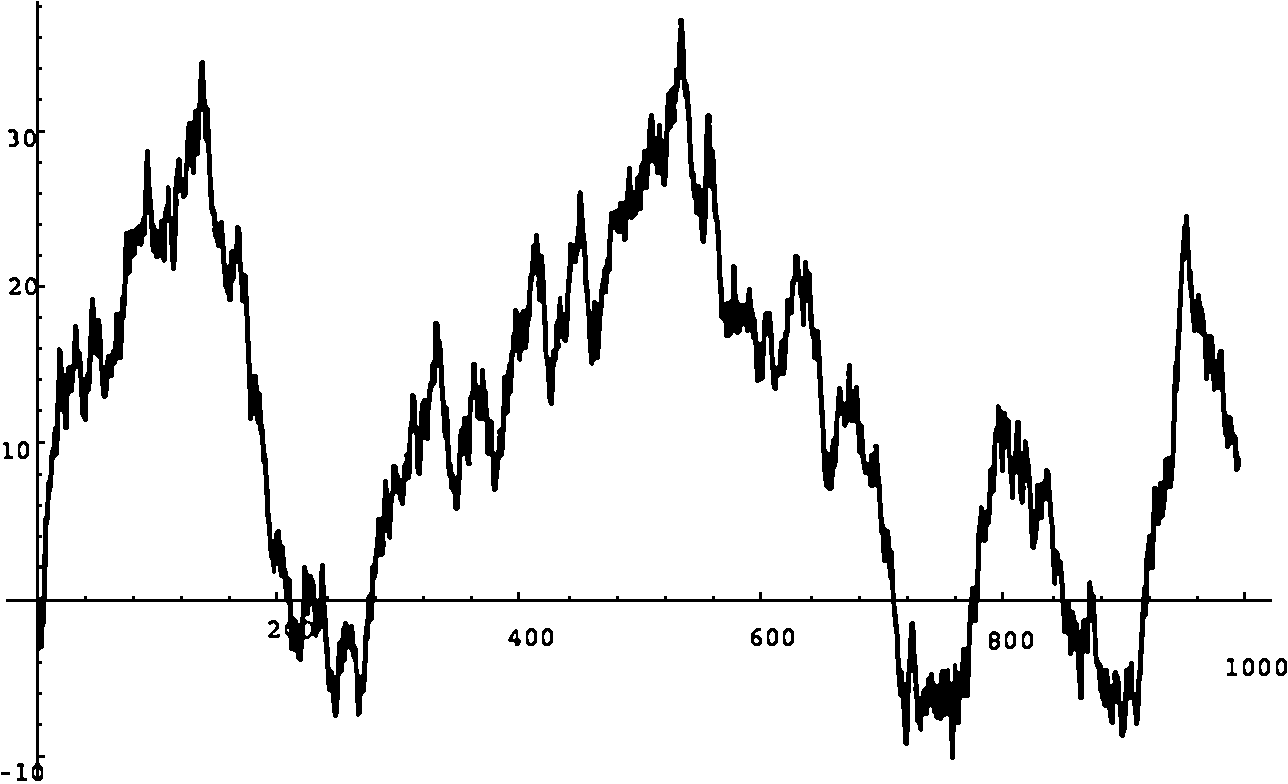
\includegraphics{Images/Img1.png}
    \bigskip
    \caption{Simulation of the graph of a one-dimensional Brownian motion $X_t$ plotted versus time.}
    \label{fig:ch1_2.1}
\end{figure}

Brownian motion has a scaling\index{Scaling} property that is extremely useful.

\mpagebreak

\begin{proposition}\label{prop:ch1_2.2}
If $(\P^x, X_t)$ is a Brownian motion starting from $x$ and $a > 0$, then $(\P^{x/a}, a^{-1}X_{a^2t})$ is a Brownian motion started from $x/a$.
\end{proposition}

\begin{proof}
We do the one-dimensional case; the higher-dimensional case is exactly similar. Since $\P^x$ is defined by translation, it is enough to consider the case $x = 0$. $a^{-1}X_{a^2t}$ is continuous in $t$, and
\[
    \Cov(a^{-1}X_{a^2t}, a^{-1}X_{a^2s}) = a^{-2}(a^2t \wedge a^2s) = s \wedge t.
\]
Using \eqref{eq:ch1_1.6}, if $t_1 \leq t_2 \leq \ldots \leq t_n$, the law of $(a^{-1}X_{a^2t_1},\ldots,a^{-1}X_{a^2t_n})$ is determined by the covariance matrix, and hence agrees with that of a Brownian motion. Since both processes are continuous, $a^{-1}X_{a^2t}$ must be a Brownian motion.
\end{proof}

\bigskip
\begin{figure}[ht]
    \centering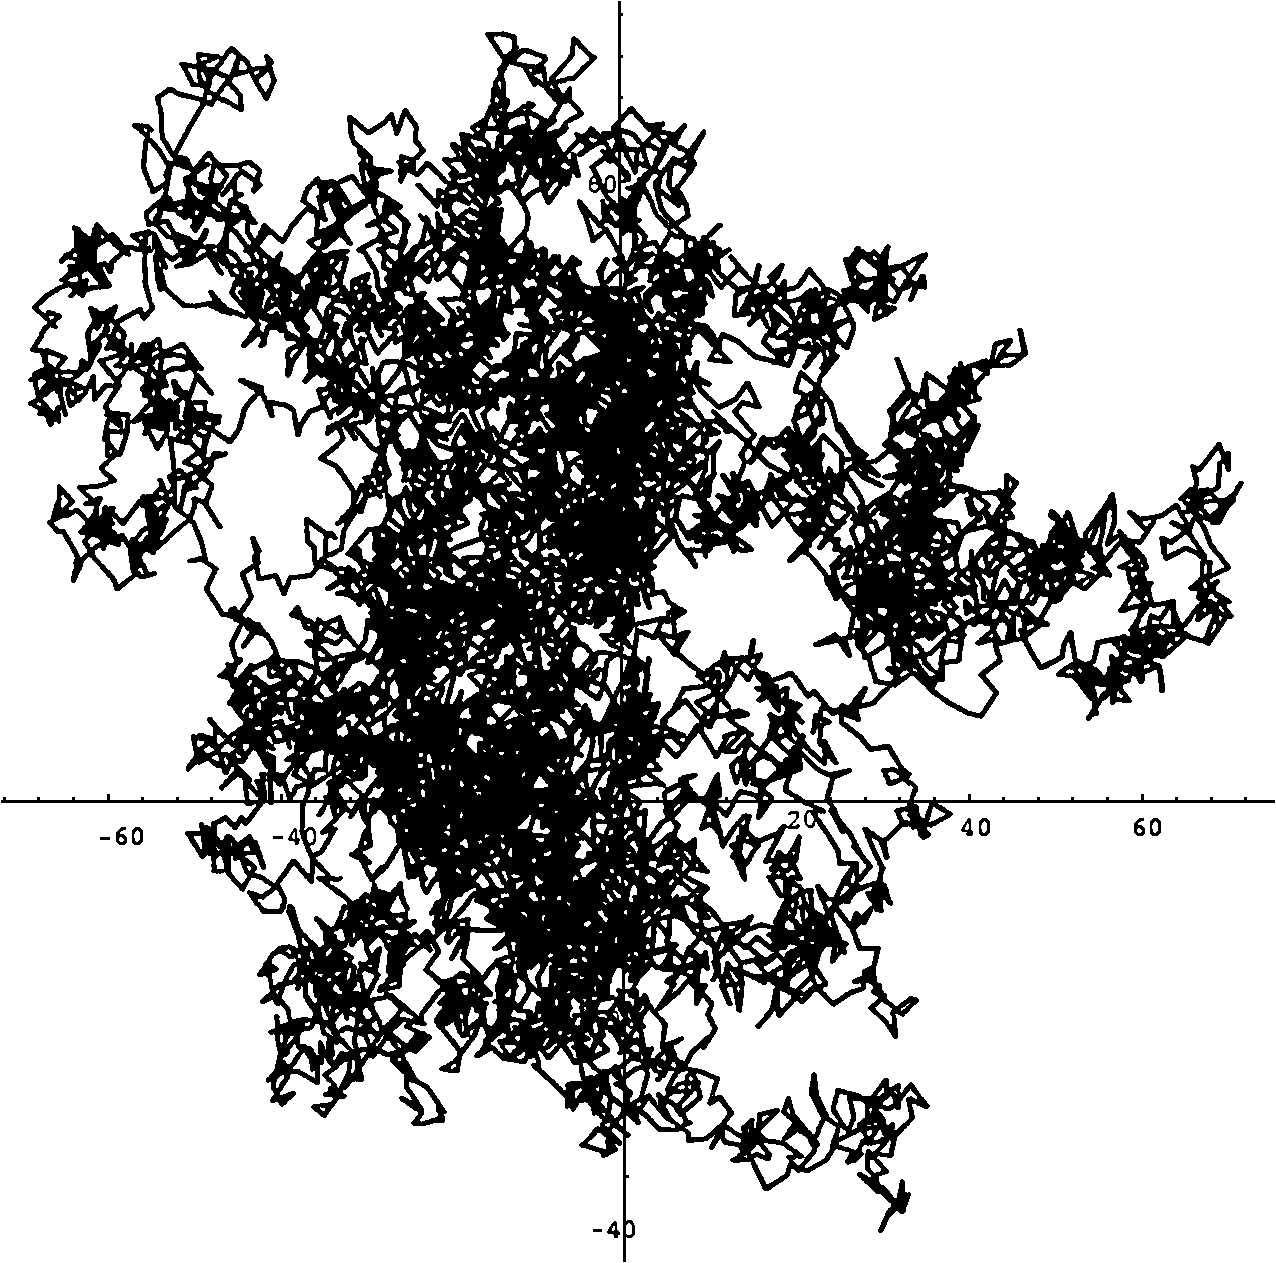
\includegraphics{Images/Img2.png}
    \caption{Simulation of the graph of a two-dimensional Brownian motion $(X_t^1, X_t^2)$.}
    \label{fig:ch1_2.2}
\end{figure}

Brownian motion is also rotationally invariant\index{Rotational invariance}.

\begin{proposition}\label{prop:ch1_2.3}
If $A$ is an orthogonal matrix, then $(\P^{Ax}, AX_t)$ is a Brownian motion starting from $Ax$.
\end{proposition}

\begin{proof}
$AX_t$ still has continuous paths and independent increments. Since $\Cov(X_t - X_s) = (t-s)I$, where $I$ is the identity matrix, then $\Cov(AX_t - AX_s) = (t-s)A^tA = (t-s)I$. By the remarks following \eqref{eq:ch1_1.6}, this shows the components of $AX_t - AX_s$ are independent and each component is a Brownian motion.
\end{proof}

\subsecbkm{ch1_sec2.2}{Construction of Brownian motion}
\index{Brownian motion!Construction of}

Let us show that there exists a process satisfying Definition \ref{def:ch1_2.1}. First we construct Brownian motion for $t \in [0,1]$. We give the Haar function\index{Haar function} construction, which is one of the quickest ways to the construction of Brownian motion.

For $i = 1,2,\ldots$, $j = 1,2,\ldots,2^{i-1}$, let $\varphi_{ij}$ be the function on $[0,1]$ that takes the value $2^{(i-1)/2}$ if $x \in [(2j-2)/2^i,(2j-1)/2^i)$, the value $-2^{(i-1)/2}$ if $x \in [(2j-1)/2^i,2j/2^i)$, and 0 otherwise. Let $\varphi_{00}$ be the function that is identically $1$. The $\varphi_{ij}$ are called the Haar functions. If $\lrang{\cdot,\cdot}$ denotes the inner product in $L^2([0,1])$, that is, $\lrang{f,g} = \int_0^1 f(x)\overline{g}(x)dx$, note the $\varphi_{ij}$ are orthogonal and have norm $1$. It is also easy to see that they form a complete orthonormal system for $L^2$: $\varphi_{00} \equiv 1$; $1_{[0,1/2)}$ and $1_{[1/2,1)}$ are both linear combinations of $\varphi_{00}$ and $\varphi_{11}$; $1_{[0,1/4)}$ and $1_{[1/4,1/2)}$ are both linear combinations of $1_{[0,1/2)}$, $\varphi_{21}$, and $\varphi_{22}$. Continuing in this way, we see that $1_{[k/2^n,(k+1)/2^n)}$ is a linear combination of the $\varphi_{ij}$s for each $n$ and each $k \leq 2^n$. Since any continuous function can be uniformly approximated by step functions whose jumps are at the dyadic rationals, linear combinations of the Haar functions are dense in the set of continuous functions, which in turn is dense in $L^2([0,1])$.

Let $\psi_{ij}(t) = \int_0^t \varphi_{ij}(s)ds$. Let $Y_{ij}$ be a sequence of independent identically distributed mean zero Gaussian random variables with variance $1$. Let
\[
    V_0(t) = Y_{00}\psi_{00}(t), \qquad V_i(t) = \sum_{j=1}^{2^{i-1}}Y_{ij}\psi_{ij}(t), \qquad i \geq 1.
\]

\begin{theorem}\label{thm:ch1_2.4}
$\sum_{i=0}^\infty V_i(t)$ converges uniformly in $t$, a.s. If we call the sum $X_t$, then $X_t$ is a Brownian motion started at $0$.
\end{theorem}

\begin{proof}
We start with the proof of convergence. We will show
\[
    \sum_{i=1}^{\infty}\P(|V_i(t)| > i^{-2}~\text{for some}~t \in [0,1]) < \infty.
\]
Then by the Borel-Cantelli lemma (Proposition \ref{prop:ch1_1.1}), with probability $1$, from some $i$ on (depending on $\omega$), $\sup_t |V_i(t)| \leq i^{-2}$. This will show $\sum_{i=0}^I V_i(t)$ converges as $I \to \infty$, uniformly over $t \in [0,1]$. Moreover, since each $\psi_{ij}(t)$ is continuous in $t$, then so is each $V_i(t)$, and we thus deduce that $X_t$ is continuous in $t$.

Now for $i \geq 1$, each $\psi_{ij}$ has a graph that looks like a little tent, and for fixed $i$, $\psi_{ij_1}(t)$ and $\psi_{ij_2}(t)$ are not both nonzero if $j_1 \neq j_2$. Also, the maximum value of $\psi_{ij}$ is $2^{-(i+1)/2}$. Hence
\begin{align*}
    \P(|V_i(t)| &> i^{-2}~\text{for some}~t \in [0,1]) \\
    &\leq \P(|Y_{ij}|\psi_{ij}(t) > i^{-2}~\text{for some}~t \in [0,1],~\text{some}~0 \leq j \leq 2^{i-1}) \\
    &\leq \P(|Y_{ij}|2^{-(i+1)/2} > i^{-2}~\text{for some}~0 \leq j \leq 2^{i-1}) \\
    &\leq (2^{i-1} + 1)\P(|Z| > 2^{(i+1)/2}i^{-2})
\end{align*}
where $Z$ is a standard mean zero variance one Gaussian random variable. By Proposition \ref{prop:ch1_1.9}, we bound the right-hand side by $2^i\exp(-2^i/4)$, which is easily checked to be summable in $i$.

This was the hard part. The $V_j$s are Gaussian and independent, so the $X_t$ are also Gaussian. It is obvious that they have mean zero. So we need only check the covariances and variances. If $f \in L^2([0,1])$, Parseval's identity says that $\lrang{f,f} = \sum_{i,j}\lrang{\varphi_{ij},f}^2$. Since $\psi_{ij}(t) - \psi_{ij}(s) = \lrang{\varphi_{ij},1_{[s,t]}}$, then $X_t - X_s = \sum_{i,j}Y_{ij}\lrang{\varphi_{ij},1_{[s,t]}}$. Since the $Y_{ij}$ are independent with mean $0$ and variance $1$,
\begin{align*}
    \E[X_t - X_s]^2 &= \E\bigg[\sum_{i,j}Y_{ij}\lrang{\varphi_{ij},1_{[s,t]}}\bigg]^2 \\
    &= \sum_{i,j}\lrang{\varphi_{ij},1_{[s,t]}}^2 \\
    &= \lrang{1_{[s,t]},1_{[s,t]}} = t-s.
\end{align*}
Similarly, $f = \sum_{i,j}\lrang{\varphi_{ij},f}\varphi_{ij}$, hence $\lrang{f,g} = \sum_{i,j}\lrang{\varphi_{ij},f}\lrang{\varphi_{ij},g}$, and therefore
\begin{align*}
    \E[X_t - X_s)&(X_r - X_q)] \\
    &= \E\bigg[\Big(\sum_{i,j}Y_{ij}\lrang{\varphi_{ij},1_{[s,t]}}\Big)\Big(\sum_{k,\ell}Y_{k\ell}\lrang{\varphi_{k\ell},1_{[q,r]}}\Big)\bigg] \\
    &= \sum_{i,j}\lrang{\varphi_{ij},1_{[s,t]}}\lrang{\varphi_{ij},1_{[q,r]}} \\
    &= \lrang{1_{[s,t]},1_{[q,r]}}.
\end{align*}
If $r \leq s$, this last inner product is $0$, and $X_t - X_s$ is a mean zero variance $t-s$ Gaussian random variable independent of $X_{r_{i+1}} - X_{r_i}$, if $r_1 \leq r_2 \leq \cdots \leq r_n \leq s$. This proves the theorem.
\end{proof}

We have constructed Brownian motion on $[0,1]$, but we also want it on $[0,\infty)$. We obtain it through a trick called time inversion\index{Time inversion}. Let $Y_t = tX_{1/t}$, $t \in [1,\infty)$. Clearly $Y_t$ is mean $0$, Gaussian, and continuous in $t$. Let us check the covariances of $Y$.
\mpagebreak
\begin{align*}
    \Cov(Y_t,Y_s) = st\Cov(X_{1/s},X_{1/t}) = st((1/t) \wedge (1/s)).
\end{align*}
This equals $s \wedge t$. So $Y_t$ is a Brownian motion for $t \geq 1$. Now let $X_t'$ be an independent Brownian motion on $[0,1]$, and let
\[
    Z_t = \begin{cases}
        X_t' & \text{if}~t \leq 1;\\
        X_1' + Y_t - Y_1 & \text{if}~t > 1.
    \end{cases}
\]
To check that $Z_t$ is a Brownian motion is routine and is left to the reader.

\subsecbkm{ch1_sec2.3}{Stopping times}

We next want to talk about stopping times. Suppose we have a stochastic process $X_t$ (think of Brownian motion as a good example) and a filtration\index{Filtration} $\FC_t$. This is an increasing collection of $\sigma$-fields. We suppose each $\FC_t$ is right continuous (i.e., $\FC_t = \FC_{t+}$ for each $t$, where $\FC_{t+} = \cap_{\epsilon>0}\FC_{t+\epsilon}$). We suppose that $X_t$ is adapted to $\FC_t$: for each $t$, $X_t$ is $\FC_t$ measurable.

\begin{definition}\label{def:ch1_2.5}
A random mapping $T$ from $\Omega$ to $[0,\infty]$ is called a stopping time if for each $t$, $(T < t) \in \FC_t$.
\end{definition}

A stopping time is also called an optional time\index{Optional times} in the Markov theory literature.

The intuition is that the process knows whether $T$ has happened by time $t$ by looking at $\FC_t$. Suppose some motorists are told to drive north on Highway $99$ in Seattle\index{Seattle} and stop at the first motorcycle shop past the second realtor after the city limits. So they drive north, pass the city limits, pass two realtors, and come to the next motorcycle shop, and stop. That is a stopping time. If they are instead told to stop at the third stop light before the city limits (and they had not been there before), they would need to drive to the city limits, then turn around and return past three stop lights. That is not a stopping time, because they have to go ahead of where they wanted to stop to know to stop there.

\begin{proposition}\label{prop:ch1_2.6}
\begin{enumerate}
    \item[]
    \item $T$ is a stopping time if and only if $(T \leq t) \in \FC_t$ for all $t$.
    \item Fixed times $t$ are stopping times.
    \item If $S$ and $T$ are stopping times, then so are $S \wedge T$ and $S \vee T$.
    \item If $T_n$ is a nondecreasing sequence of stopping times, then so is $T = \sup_n T_n$.
    \item If $T_n$ is a nonincreasing sequence of stopping times, then so is $T = \inf_n T_n$.
    \item If $S$ is a stopping time, then so is $S + t$.
\end{enumerate}
\end{proposition}

\begin{proof}
These follow from the definitions. We will do (a), leaving the rest as Exercise \ref{ex:ch1_8}. If $T$ is a stopping time, then $(T \leq t) = \cap_{n>N}(T < t + 1/n) \in \cap_{n>N}\FC_{t+1/n}$ for each $N$. So $(T \leq t) \in \FC_{t+} = \FC_t$. On the other hand, if $(T \leq t) \in \FC_t$ for all $t$, then $(T < t) = \cup_{n=1}^\infty(T \leq t - 1/n) \in \FC_t$, since $\FC_t$ is increasing.
\end{proof}

Among the kinds of stopping times we will be interested in are the first times that $X_t$ hits a set $A$ or leaves a set $A$ (the second is the same as hitting $A^c$). In the notation we will use throughout the rest of the book, let
\begin{equation}\label{eq:ch1_2.3}
    T_A = \inf\{t > 0 : X_t \in A\}\index{TA@$T_A$}\index{Hitting times}
\end{equation}
and
\begin{equation}\label{eq:ch1_2.4}
    \tau_A = \inf\{t > 0 : X_t \notin A\}.\index{À6@$\tau_A$}\index{Exit times}
\end{equation}
Of course, $T_A = \tau_{A^c}$ and $\tau_A = T_{A^c}$.

It will turn out that $T_A$ and $\tau_A$ are stopping times for all Borel measurable sets $A$, but that is a hard result, and we only need it in that generality for Chap.\ \ref{ch2}. We leave the general result to Sect.\ \chapref[II]{ch2_sec2}; here we only prove the result we need for the other chapters, namely, the cases when $A$ is either open or closed.

\begin{proposition}\label{prop:ch1_2.7}
\begin{enumerate}
    \item[]
    \item If $A$ is an open set, $T_A$ is a stopping time.
    \item If $A$ is a closed set, $T_A$ is a stopping time.
\end{enumerate}
\end{proposition}

% Note: it seems that T in the proof of (a) should be T_A.

\begin{proof}
Suppose $A$ is open. If $T_A < t$, then for some $s$ less than $t$, we have $X_s \in A$. Since the paths are continuous (right continuity would do), there is a rational $q < t$ with $X_q \in A$. Hence
\[
    (T_A < t) = \bigcup_{q<t,q~\text{rational}} (X_q \in A) \in \FC_t,
\]
which proves (a).

If $A$ is closed, let $A_n = \{x : \dist(x,A) < 1/n\}$. The $A_n$s are open, so $T_{A_n}$ is an increasing sequence of stopping times, hence by Proposition \ref{prop:ch1_2.6}, $T = \sup_n T_{A_n}$ is a stopping time. Since $T_A \geq T_{A_n}$ for each $n$, then $T_A \geq T$. If $T = \infty$, then $T_A$ must also equal $\infty$. If $T < \infty$, by the continuity of paths, $X_T = \lim X(T_{A_n})$. Since $X(T_{A_n})$ is in the closure of $A_m$ if $n \geq m$, it follows that $X_T$ is also, for each $m$. That implies $X_T \in A$, or $T_A \leq T$. In either case, $T_A = T$, which proves (b).
\end{proof}

\begin{proposition}\label{prop:ch1_2.8}
$\P^x(X(T_{B(x,r)}) \in dy)$ is normalized surface measure on $\partial B(x,r)$.
\end{proposition}

\begin{proof}
By the rotational invariance of Brownian motion (Proposition \ref{prop:ch1_2.3}), if $C$ is any Borel subset of $\partial B(0,r)$ and $A$ any orthogonal matrix,
\begin{align*}
    \P^0(X(\tau_{B(0,r)}) \in C) &= \P^0(AX(\tau_{B(0,r)}) \in C) \\
    &= \P^0(X(\tau_{B(0,r)}) \in A^{-1}C).
\end{align*}
\mnewpage
Therefore $\P^0(X(\tau_{B(0,r)}) \in dy)$ must be surface measure on $\partial B(0,r)$, normalized to have total mass $1$. The result follows by translation invariance.
\end{proof}

It follows that if $f$ is a function defined on the boundary of $B(x,r)$, then
\[
    \E^x f(X_{\tau_{B(x,r)}}) = \int_{\partial B(x,r)} f(y)\sigma(dy),
\]
where $\sigma$ is normalized surface measure on the boundary of $B(x,r)$. We will use this fact in the next chapter as part of our solution of the Dirichlet problem.

\section{Markov properties}\label{ch1_sec3}

\subsecbkm{ch1_sec3.1}{The Markov Property}

Before starting out on the Markov property\index{Markov property} and strong Markov properties, let us first introduce some notation. Define $\FC_t^{00} = \sigma(X_s; s \leq t)$, $t \in [0,\infty]$\index{F3@$\FC_t^{00}$}. We let $\FC_t^0$\index{F2@$\FC_t^0$} be the completion of $\FC_t^{00}$, but we need to be careful what we mean by completion here, because we have more than one probability measure floating around. Let $\FC_t^0$ be the $\sigma$-field generated by $\FC_t^{00}$ and $\NC$, where $\NC$ is the collection of sets that are $\P^x$ null for every $x \in \R^d$. Finally, let $\FC_t = \FC_{t+}^0 = \cap_{\epsilon>0}\FC_{t+\epsilon}^0$. Ultimately, we will work only with $\FC_t$, but we need the other two $\sigma$-fields at intermediate stages. The reason for worrying about which filtrations to use is that $\FC_t^{00}$ is too small to include many interesting sets (such as those arising in the law of the iterated logarithm), while if the filtration is too large, the Markov property will not hold for that filtration.

We will denote expectation with respect to $\P^x$ by $\E^x$. Let us explain the notation $\E^{X_s}Y$. This is the random variable $\varphi(X_s)$, where $\varphi(y) = \E^y Y$. Thus, for example, $\E^x\E^{X_s}Y = \E^x\varphi(X_s)$.

Let
\begin{equation}\label{eq:ch1_3.1}
    p(t,x,y) = (2\pi t)^{-d/2}e^{-|x-y|^2/2t}, \qquad x,y \in \R^d, \qquad t > 0.
\end{equation}
The corresponding operator $P_t$ on functions is given by
\begin{equation}\label{eq:ch1_3.2}
    P_tf(x) = \int f(y)p(t,x,y)dy.
\end{equation}
Note that if $f$ is bounded and $t > 0$, then $P_tf(x)$ is continuous in $x$ by the continuity of $p(t,x,y)$ and dominated convergence.

If $\Omega$ is the set of continuous functions from $[0,\infty)$ to $\R^d$, we define the shift operators\index{Shift operators} $\theta_t : \Omega \to \Omega$ by
\[
    \theta(\omega)(s) = \omega(t + s).
\]
Then
\[
    X_s \circ \theta_t(\omega) = X_s(\theta_t\omega) = \theta_t\omega(s) = \omega(s + t) = X_{t+s}(\omega)
\]
if the $X_s$ process is given by coordinate maps as in \eqref{eq:ch1_2.1}. Even if we are not in this canonical setup, we will suppose there exist shift operators mapping $\Omega$ into itself so that
\begin{equation}\label{eq:ch1_3.3}
    X_s \circ \theta_t = X_{s+t}.
\end{equation}

We can now state the Markov property, at least the one for $\FC_t^{00}$.

\begin{proposition}\label{prop:ch1_3.1}
If $Y$ is bounded and $\FC_\infty^{00}$ measurable and $(\P^x, X_t)$ is a Brownian motion, then
\[
    \E^x[Y \circ \theta_s\mid \FC_s^{00}] = \E^{X_s}Y, \qquad \textnormal{a.s.}~(\P^x).
\]
\end{proposition}

For the first time through for this and the next subsection, it would be a good idea to read the statements of the results and the examples but to skip the proofs.

Before proving this proposition, let us first give some examples. For example, if $Y = f(X_t)$, Proposition \ref{prop:ch1_3.1} says that
\[
    \E^x[f(X_{t+s})\mid \FC_s^{00}] = \E^x[f(X_t) \circ \theta_s\mid \FC_s^{00}] = \E^{X_s}f(X_t).
\]
As another example,
\begin{align*}
    \P^x(X_t \in [4,5]~\text{for some}~t &\in [3,4] \mid \FC_2^{00}) \\
    &= \P^{X_2}[X_t \in [4,5]~\text{for some}~t \in [1,2]].
\end{align*}

We start the proof of Proposition \ref{prop:ch1_3.1} by proving a lemma, which is just the first example given above.

\begin{lemma}\label{lem:ch1_3.2}
If $f$ is bounded and Borel measurable,
\[
    \E^x[f(X_t) \circ \theta_s\mid \FC_s^{00}] = \E^{X_s}f(X_t), \qquad \textnormal{a.s.}~(\P^x).
\]
\end{lemma}

\begin{proof}
It will suffice to prove $\E^x[f(X_{t+s})\mid \FC_s^{00}] = \E^{X_s}f(X_t)$ when $f(x) = e^{\im u\cdot x}$, where $u\cdot x$ is the inner product in $\R^d$, for we can then take linear combinations and limits. Using independent increments, the fact that $X_{t+s} - X_s$ is a $\NC(0,t)$, and \eqref{eq:ch1_1.6}, we have
\begin{align*}
    \E^x\big[e^{\im u\cdot X_{t+s}}\mid \FC_s^{00}\big] &= \E^x\big[e^{\im u\cdot(X_{t+s}-X_s)}\mid \FC_s^{00}\big]e^{\im u\cdot X_s} \\
    &= \E^x\big[e^{\im u\cdot(X_{t+s}-X_s)}\big]e^{\im u\cdot X_s} \\
    &= e^{-|u|^2t/2}e^{\im u\cdot X_s}.
\end{align*}
On the other hand, for any $y$,
\mpagebreak
\begin{align*}
    \E^y e^{\im u\cdot X_t} = \E^0 e^{\im u\cdot X_t}e^{\im u\cdot y} = e^{-|u|^2t/2}e^{\im u\cdot y}.
\end{align*}
Replacing $y$ by $X_s$ gives the desired equality.
\end{proof}

\begin{proof}[Proof of Proposition \ref{prop:ch1_3.1}]
By linearity and limits, it suffices to show the equality when $Y = \prod_{j=1}^n f_j(X_{t_j})$, where the $f_j$ are bounded and $s \leq t_1 \leq \ldots \leq t_n$. We will prove it for such $Y$ by induction on $n$. The case $n = 1$ was Lemma \ref{lem:ch1_3.2}, so we suppose the equality for $n$ and prove it for $n + 1$.

Let $V = \prod_{j=2}^{n+1} f_j(X_{t_j-t_1})$, $h(y) = \E^y V$. By the induction hypothesis,
\begin{align*}
    \E^x\Big[\prod_{j=1}^{n+1}f_j(X_{t_j})\mid \FC_s^{00}\Big] &= \E^x\Big[\E^x[V \circ \theta_{t_1}\mid \FC_{t_1}^{00}]f_1(X_{t_1})\mid \FC_s^{00}\Big] \\
    &= \E^x\Big[(\E^{X_{t_1}}V)f_1(X_{t_1})\mid \FC_s^{00}\Big] \\
    &= \E^x[(hf_1)(X_{t_1})\mid \FC_s^{00}].
\end{align*}
By Lemma \ref{lem:ch1_3.2}, this is $\E^{X_s}[(hf_1)(X_{t_1-s})]$. For any $y$,
\begin{align*}
    \E^y[(hf_1)(X_{t_1-s})] &= \E^y[(\E^{X_{t_1-s}}V)f_1(X_{t_1-s})] \\
    &= \E^y\Big[\E^y[V \circ \theta_{t_1-s}\mid \FC_{t_1-s}^{00}]f_1(X_{t_1-s})\Big] \\
    &= \E^y[(V \circ \theta_{t_1-s})f_1(X_{t_1-s})].
\end{align*}
If we replace $V$ by its definition, replace $y$ by $X_s$, and use the definition of $\theta_{t_1-s}$, we get the desired equality for $n+1$ and hence the induction step and the proposition.
\end{proof}

A moment's thought shows that adding null sets does not hurt anything, so we have the following corollary.

\begin{corollary}\label{cor:ch1_3.3}
If $Y$ is bounded and is $\FC_\infty^0$ measurable, then
\[
    \E^x[Y \circ \theta_t\mid \FC_t^0] = \E^{X_t}Y, \qquad \textnormal{a.s.}~ (\P^x).
\]
\end{corollary}

The next step is to go from $\FC_t^0$ to $\FC_t$.

\begin{theorem}\label{thm:ch1_3.4}
If $Y$ is bounded and $\FC_\infty$ measurable and $(\P^x, X_t)$ is a Brownian motion,
\[
    \E^x[Y \circ \theta_t\mid \FC_t] = \E^{X_t}Y.
\]
\end{theorem}

\begin{proof}
Just as in the proof of Proposition \ref{prop:ch1_3.1}, it suffices to prove the result for $Y$ of the form $f(X_t)$ and then use induction. By a limiting process, we may also assume $f$ is continuous.

If $A \in \FC_s = \FC_{s+}^0$, then $A \in \FC_{s+\epsilon}^0$ for every $\epsilon > 0$. So by the Markov property with respect to $\FC_{s+\epsilon}^0$,
\mpagebreak
\begin{align*}
    \E^x[f(X_{t+s+\epsilon});A] = \E^x[P_tf(X_{s+\epsilon});A].
\end{align*}

If we let $\epsilon \to 0$, the left-hand side converges to $\E^x[f(X_{t+s});A]$ by dominated convergence and the continuity of $f$ and $X$. As we noted following \eqref{eq:ch1_3.2}, $P_tf$ is continuous. The right-hand side converges to $\E^x[P_tf(X_s);A]$ by dominated convergence and the continuity of $P_tf$ and $X$. Sorting out the notation, we see we have exactly what we wanted.
\end{proof}

\subsecbkm{ch1_sec3.2}{Zero-one laws}

We show that going from $\FC_s^0$ to $\FC_s$ did not really change anything essential.

\begin{proposition}\label{prop:ch1_3.5}
$\FC_s = \FC_s^0$.
\end{proposition}

\begin{proof}
Let $Y = \prod_{j=1}^n f_j(X_{t_j})$. If $t_j \leq s < t_{j+1}$, let $Y_1 = \prod_{\{j:t_j \leq s\}} f_j(X_{t_j})$ and $Y_2 = \prod_{\{j:t_j>s\}} f_j(X_{t_j})$. Then
\[
    \E^x[Y\mid \FC_{s+}^0] = Y_1\E^{X_s}Y_2,
\]
which is $\FC_s^0$ measurable.

By linearity and limits, $\E^x[Y\mid \FC_{s+}^0]$ is $\FC_s^0$ measurable whenever $Y \in \FC_\infty^0$. If $A \in \FC_s = \FC_{s+}^0$, letting $Y = 1_A$ shows that $A \in \FC_s^0$.
\end{proof}

\begin{corollary}[Blumenthal zero-one law\index{Blumenthal zero-one law}]\label{cor:ch1_3.6}
If $A \in \FC_0$, then $\P^x(A)$ equals either $0$ or $1$.
\end{corollary}

\begin{proof}
If $A \in \FC_0$, then under $\P^x$,
\[
    1_A = \E^x[1_A\mid \FC_{0+}] = \E^{X_0}1_A = \P^x(A).
\]
Hence $\P^x(A) = 1_A \in \{0,1\}$.
\end{proof}

As an example of the use of the zero-one law\index{Zero-one law}, we show $\P^0(T_{(0,\infty)} = 0) = 1$, i.e., Brownian motion immediately enters the positive real axis. Since by symmetry it also enters the negative reals immediately, the behavior of Brownian motion is rather peculiar. The explanation is that Brownian motion oscillates between positive and negative values in every neighborhood of the origin on the time axis. For a more precise statement, see the law of the iterated logarithm (Exercise \ref{ex:ch1_4}). To show the assertion about $T_{(0,\infty)}$, for any $t$, $\P^0(T_{(0,\infty)} \leq t) \geq \P^0(X_t > 0)$, which by the symmetry of the $\NC(0,t)$ distribution is $1/2$. Letting $t \downarrow 0$, $\P^0(T_{(0,\infty)} = 0) \geq 1/2$. By the zero-one law the probability, then, must be one.

As another example, let $\varphi(t)$ be any nondecreasing function with $\varphi(0) = 0$. Then the event $(\limsup_{t\to 0} X_t/\varphi(t) > a)$ is in $\FC_0$ and hence has probability $0$ or $1$ for each $a$. Therefore $\limsup_{t\to 0} X_t/\varphi(t)$ is constant, a.s.\ (the constant might be $0$ or $\infty$).

\subsecbkm{ch1_sec3.3}{Semigroups}
\index{Semigroups}

The Markov property says that for Brownian motion $\E^x[\E^{X_s}f(X_t)]= \E^xf(X_{s+t})$. This can be rewritten as $P_{s+t}f(x) = P_s(P_tf)(x)$ or
\begin{equation}\label{eq:ch1_3.4}
    P_{s+t} = P_sP_t.
\end{equation}
Hence the operators form a semigroup (in the functional analysis sense). Since the paths of Brownian motion are continuous, it is easy to see that the semigroup is strongly continuous\index{Strongly continuous} with respect to the space of continuous functions (that is, $P_tf \to P_sf$ uniformly if $f$ is continuous and $t \downarrow s$). Given such a semigroup, it is common to compute the infinitesimal generator\index{Infinitesimal generator}
\[
    \lim_{t\downarrow 0} \frac{P_tf - f}{t}
\]
for some collection of $f$s and where the limit is in some appropriate norm. In Exercise \ref{ex:ch1_6}, we show that the infinitesimal generator of Brownian motion in $\R^d$ has the bounded $C^2$ functions as its domain, and on such functions it is $(1/2)\Delta$\index{À3@$\Delta$}, one half the Laplacian\index{Laplacian}.

If we let $U^\lambda f(x) = \int_0^\infty e^{-\lambda t}P_tf(x)dt$, then
\[
    U^\lambda U^\beta f(x) = \int_0^\infty e^{-\lambda t} \int_0^\infty e^{-\beta s}P_tP_sf(x)ds\,dt.
\]
Using the semigroup property and a change of variables, this is
\begin{align*}
    \int_0^\infty e^{(\beta-\lambda)t} \int_t^\infty e^{-\beta s}&P_sf(x)ds\,dt \\
    &= \int_0^\infty P_sf(x)e^{-\beta s} \int_0^s e^{(\beta-\lambda)t}dt\,ds \\
    &= \frac{U^\lambda f(x) - U^\beta f(x)}{\beta - \lambda}.
\end{align*}
The equation
\begin{equation}\label{eq:ch1_3.5}
    (\beta - \lambda)U^\lambda U^\beta = U^\lambda - U^\beta
\end{equation}
is called the resolvent equation\index{Resolvent!Equation}.

Suppose $f$ is smooth, say $C^\infty$ with compact support. By translation invariance, $\partial P_tf(x)/\partial x^i = P_t(\partial f/\partial x^i)$, or $P_tf$ is also smooth, hence so is $U^\lambda f$. Let $g$ be $C^\infty$ with compact support.

Applying Green's first identity\index{Green's identities} (see Sect.\ \chapref[II]{ch2_sec1}) on $B(0,N)$, and letting $N \to \infty$, we see
\[
    -(1/2)\int_{\R^d} g(x)(\Delta U^\lambda f(x))dx = (1/2)\int_{\R^d} \nabla U^\lambda f(x) \cdot \nabla g(x)dx.
\]
If we write $\EC(g,h)$ for $1/2\int_{\R^d} \nabla g(x) \cdot \nabla h(x)dx$, we have
\mpagebreak
\begin{equation}\label{eq:ch1_3.6}
    \EC(g,U^\lambda f) = -(1/2)\int_{\R^d} g(x)(\Delta U^\lambda f(x))dx.
\end{equation}
$\EC$ is an example of a Dirichlet form\index{Dirichlet form} and \eqref{eq:ch1_3.6} shows that the Dirichlet form corresponding to Brownian motion is $\EC(f,f) = (1/2)\int |\nabla f|^2(x)dx$. One can show that the domain of $\EC$ is $\{f : \int|\nabla f|^2(x)dx < \infty, f \to 0$ as $|x| \to \infty\}$.

\subsecbkm{ch1_sec3.4}{Strong Markov property}

In the previous section we defined stopping times. Given a stopping time $T$, the $\sigma$-field of events known up to time $T$ is defined to be
\begin{equation}
    \FC_T = \{A \in \FC_\infty : A \cap (T \leq t) \in \FC_t~\text{for all}~t > 0\}\index{F1@$\FC_T$}
\end{equation}\label{eq:ch1_3.7}
(see Exercise \ref{ex:ch1_9}). We define $\theta_T$ by $\theta_T(\omega)(t) = \omega(T(\omega) + t)$. So, for example, $X_t \circ \theta_T(\omega) = X_{T(\omega)+t}(\omega)$ and $X_T(\omega) = X_{T(\omega)}(\omega)$.

Now that we have these definitions (admittedly a bit opaque at this stage---be patient until we reach the examples), we can state the strong Markov property\index{Strong Markov property}. On the first reading, skip the proof of Theorem \ref{thm:ch1_3.7}.

\begin{theorem}\label{thm:ch1_3.7}
If $Y$ is bounded and $\FC_\infty$ measurable and $(\P^x, X_t)$ is a Brownian motion, then
\[
    \E^x[Y \circ \theta_T\mid \FC_T] = \E^{X_T}Y, \qquad \textnormal{a.s.}~\text{on}~(T < \infty).
\]
\end{theorem}

\begin{proof}
Following the proofs of Proposition \ref{prop:ch1_3.1} and Theorem \ref{thm:ch1_3.4}, it is enough to prove
\[
    \E^x[f(X_{T+t})\mid \FC_T] = \E^{X_T}f(X_t)
\]
for $f$ bounded and continuous. Define $T_n$ by $T_n(\omega) = k/2^n$ if $T(\omega) \in [(k-1)/2^n,k/2^n)$. Then $T_n$ are stopping times decreasing to $T$ on the set $(T < \infty)$.

If $A \in \FC_T$, then $A\in\FC_{T_n}$. Therefore $A \cap (T_n = k/2^n) \in \FC_{k/2^n}$ and we have
\begin{align*}
    \E^x[f(X_{T_n+t});A \cap (T_n = k/2^n)] &= \E^x[f(X_{t+k/2^n});A \cap (T = k/2^n)] \\
    &= \E^x[\E^{X_{k/2^n}}f(X_t);A \cap (T_n = k/2^n)] \\
    &= \E^x[\E^{X_{T_n}}f(X_t);A \cap (T_n = k/2^n)].
\end{align*}
Then
\begin{align*}
    \E^x[f(X_{T_n+t});A \cap (T < \infty)] &= \sum_{k=1}^\infty \E^x[f(X_{T_n+t});A \cap (T_n = k/2^n)] \\
    &= \sum_{k=1}^\infty \E^x\big[\E^{X_{T_n}}f(X_t);A \cap (T_n = k/2^n)\big] \\
    &= \E^x[\E^{X_{T_n}}f(X_t);A \cap (T < \infty)].
\end{align*}

\mpagebreak

Now let $n \to \infty$. $\E^x[f(X_{T_n+t});A \cap (T < \infty)] \to \E^x[f(X_T);A \cap (T < \infty)]$ by dominated convergence and the continuity of $f$ and $X_t$. On the other hand, $\E^{X_{T_n}}f(X_t) = P_tf(X_{T_n}) \to P_tf(X_T) = \E^{X_T}f(X_t)$ since $P_tf$ is, as we saw following \eqref{eq:ch1_3.2}, a continuous function.
\end{proof}

The first example we give is the key to the probabilistic solution to the Dirichlet problem\index{Dirichlet problem}. Let $D$ be an open domain, $\tau_D = \inf\{t : X_t \notin D\}$, $f$ a bounded function on $\partial D$, and $u(x) = \E^x f(X_{\tau_D})$. Let $x \in D$, $\delta < \dist(x,\partial D)$, and $S = \inf\{t : X_t \notin B(x,\delta)\}$. If $\omega$ is a continuous curve starting at $x$ and going until the boundary of $D$, then $\theta_S(\omega)$ is the portion of that same curve starting from the first time $\omega$ hits the ball of radius $\delta$ about $x$ and continuing until the boundary of $D$. So the location where the longer curve and shorter piece of the curve hit the boundary of $D$ will be the same place, and hence $X_{\tau_D} \circ \theta_S = X_{\tau_D}$. (See Fig.\ \ref{fig:ch1_3.1}.) Although we do not need it here, the time for the longer curve to hit the boundary is equal to the time for the curve to first hit the ball plus the time for the shorter piece of the curve to go from the ball to the boundary of $D$, or $\tau_D = S + \tau_D \circ \theta_S$. We then have
\begin{align}\label{eq:ch1_3.8}
    u(x) &= \E^x f(X_{\tau_D}) = \E^x\big[\E^x[f(X_{\tau_D}) \circ \theta_S\mid \FC_S]\big] \\
    &= \E^x\E^{X_S}f(X_{\tau_D}) = \E^xu(X_S). \notag
\end{align}

\bigskip
\begin{figure}[ht]
    \centering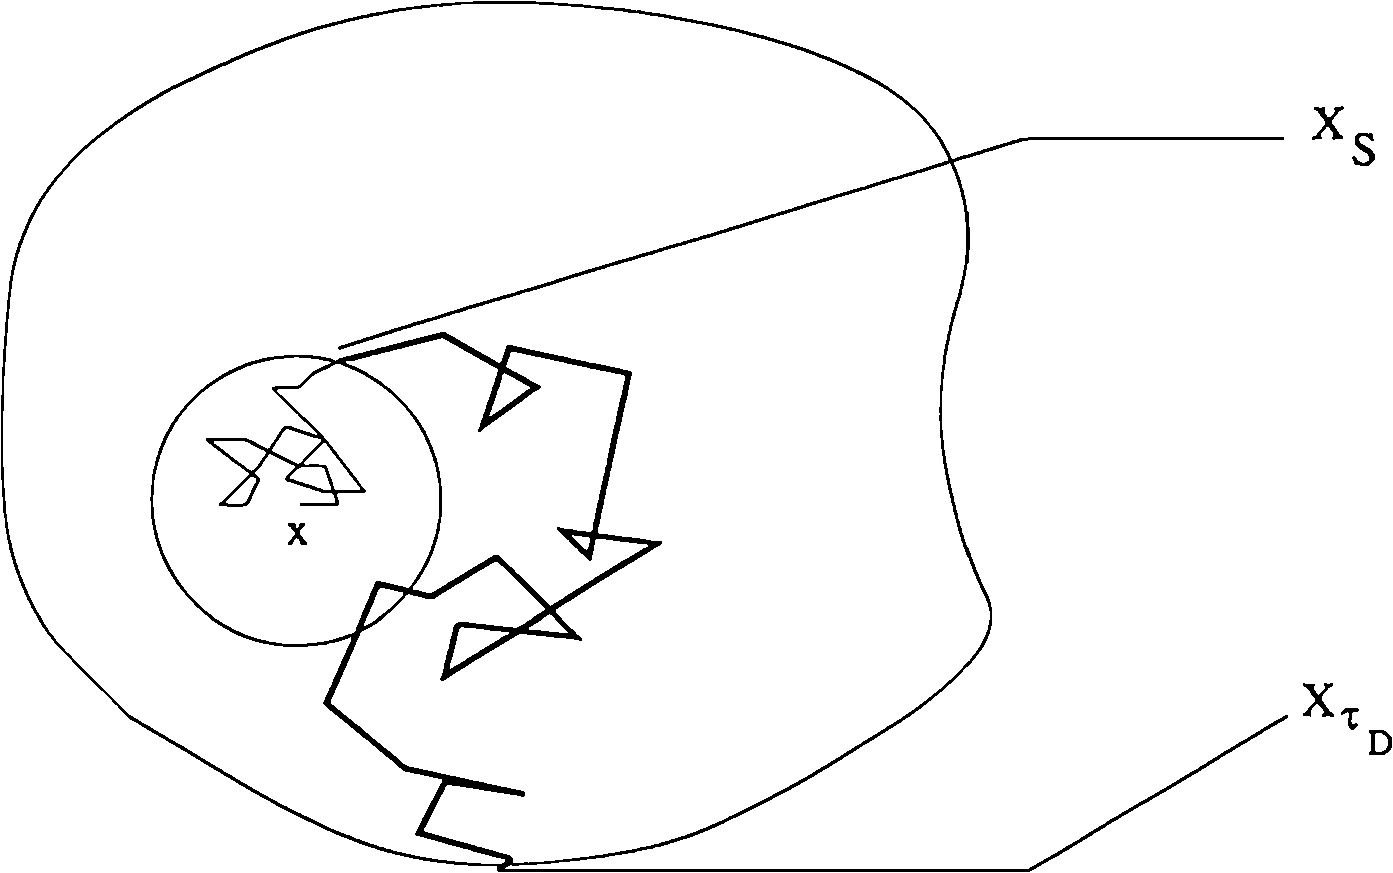
\includegraphics{Images/Img3.png}
    \caption{Graph of Brownian motion until exiting $D$.}
    \label{fig:ch1_3.1}
\end{figure}

(To anticipate Chap.\ \ref{ch2} slightly, the connection with the Dirichlet problem is that since the distribution of $X_S$ is uniform on the surface of $B(x,\delta)$, \eqref{eq:ch1_3.8} says that $u(x)$ is the average of its values on the surfaces of small balls centered at $x$. This implies that $u$ is harmonic.)

For a second example, let $D$ be a domain that has the property that there exists $c > 0$ such that
\[
    \inf_{x\in D} \P^x(X(\tau_{B(x,2)}) \notin D) \geq c.
\]
The strip $[0,1] \times \R^{d-1}$ has this property, for example, because the $\P^x$ law of $X(\tau_{B(x,2)})$ is uniform on $\partial B(x,2)$. Let $S_1$ be the first time $X_t$ moves a distance more than 2 from its starting point, $S_2$ the first time after $S_1$ that $X_t$ moves a distance at least 2 from $X_{S_1}$, and so on. We can write $S_1 = \inf\{t > 0 : |X_t - X_0| \geq 2\}$ and $S_2 = \inf\{t > S_1 : |X_t - X_{S_1}| \geq 2\}$, and so on, but a more compact way to write this is to define $S_1$ as we just did and then define $S_2 = S_1 + S_1 \circ \theta_{S_1}$, $S_3 = S_2 + S_1 \circ \theta_{S_2}$, etc. To see this, note that the length of time $S_2 - S_1$ for the $X_t$ curve to move a distance 2 is the same as the time for $X_t \circ \theta_{S_1}$, the portion of the curve with the first $S_1$ units discarded, to move a distance $2$.

The probability that the process can move a distance $2$ at least $k$ times before exiting $D$ can be bounded by
\begin{align*}
    \P^x(S_k < \tau_D) &\leq \P^x(S_{k-1} < \tau_D, S_1 \circ \theta_{S_{k-1}} < \tau_D \circ \theta_{S_{k-1}}) \\
    &= \E^x\big[\P^x(S_1 \circ \theta_{S_{k-1}} < \tau_D \circ \theta_{S_{k-1}}\mid \FC_{S_{k-1}});S_{k-1} < \tau_D\big]
\end{align*}
since on $(S_{k-1} < \tau_D)$, $\tau_D = S_{k-1} + \tau_D \circ \theta_{S_{k-1}}$ as in the first example, and $(S_{k-1} < \tau_D)$ is $\FC_{S_{k-1}}$ measurable.

By the strong Markov property and the fact that $X_{S_{k-1}} \in D$ on $(S_{k-1} < \tau_D)$,
\begin{align*}
    \P^x(S_k < \tau_D) &\leq \E^x\big[\P^{X(S_{k-1})}(S_1 < \tau_D);S_{k-1} < \tau_D\big] \\
    &\leq (1-c)\P^x(S_{k-1} < \tau_D).
\end{align*}
Induction then gives $\P^x(S_k < \tau_D) \leq (1-c)^k$.

A third example is to let $f : B(0,R) \to [0,\infty)$, let $S = \tau_{B(0,R)}$, and let $A = \sup_{x\in B(0,R)} \E^x \int_0^S f(X_s)ds$. Assume $A < \infty$. We want to show
\begin{equation}\label{eq:ch1_3.9}
    \sup_{x\in B(0,R)} \P^x\Big(\int_0^S f(X_s)ds \geq 2kA\Big) \leq 2^{-k}.
\end{equation}

Let $U_1 = \inf\{t : \int_0^{t\wedge S} f(X_s)ds \geq 2A\}$, and again $U_{i+1} = U_i + U_1 \circ \theta_{U_i}$. The event $\P^x(\int_0^S f(X_s)ds \geq 2kA)$ is bounded by
\begin{align*}
    \P^x(U_k \leq S) &\leq \P^x(U_{k-1} \leq S, U_1 \circ \theta_{U_{k-1}} \leq S \circ \theta_{U_{k-1}}) \\
    &= \E^x\big[\P^x(U_1 \circ \theta_{U_{k-1}} \leq S \circ \theta_{U_{k-1}}\mid \FC_{U_{k-1}});U_{k-1} \leq S\big] \\
    &= \E^x\big[\P^{X(U_{k-1})}(U_1 \leq S);U_{k-1} \leq S\big].
\end{align*}
If $U_{k-1} \leq S$, then $X_{U_{k-1}} \in B(0,R)$. If $y \in B(0,R)$,
\mpagebreak
\begin{align*}
    \P^y(U_1 \leq S) \leq \P^y\Big(\int_0^S f(X_s)ds \geq 2A\Big) \leq \frac{\E^y \int_0^S f(X_s)ds}{2A} \leq 1/2
\end{align*}
by Chebyshev's inequality. So then
\[
    \P^x(U_k \leq S) \leq (1/2)\P^x(U_{k-1} \leq S)
\]
and \eqref{eq:ch1_3.9} follows by induction.

A fourth example: \hspace{-0.1em}Suppose $A$ and $B$ are closed sets and $\inf_{x\in A} \P^x(T_B<\allowbreak\infty) \geq c$. (Since $d$-dimensional Brownian motion tends to $\infty$ as $t \to \infty$ if $d \geq 3$, it is possible $\sup_{x\in A} \P^x(T_B < \infty) < 1$.) Then for any $y$,
\[
    \P^y(T_B < \infty) \geq c\P^y(T_A < \infty).
\]
This follows because if $T_A < T_B$, then $T_B = T_A + T_B \circ \theta_{T_A}$. Since $X_{T_A} \in A$,
\begin{align*}
    \P^y(T_B < \infty) &\geq \P^y(T_A < T_B < \infty) \geq \P^y(T_A < \infty, T_B \circ \theta_{T_A} < \infty) \\
    &= \E^y\big[\P^y(T_B \circ \theta_{T_A} < \infty\mid \FC_{T_A}); T_A < \infty\big] \\
    &= \E^y\big[\P^{X(T_A)}(T_B < \infty); T_A < \infty\big] \\
    &\geq c\P^y(T_A < \infty).
\end{align*}

\subsecbkm{ch1_sec3.5}{Reflection principle}

Let $X_t$ be one-dimensional Brownian motion and $M_t = \sup_{s\leq t} X_s$. Another use of the Markov property is to calculate the joint law of $X_t$ and $M_t$.

\index{Reflection principle}

\begin{theorem}\label{thm:ch1_3.8}
If $a \geq b$,
\begin{equation}\label{eq:ch1_3.10}
    \P^0(M_t \geq a, X_t < b) = \P^0(X_t > 2a - b)
\end{equation}
and
\begin{equation}\label{eq:ch1_3.11}
    \P^0(M_t \geq a) = 2\P^0(X_t > a).
\end{equation}
\end{theorem}

\begin{proof}
Let $S_a = \inf\{s : X_s \geq a\}$. Then
\begin{align}\label{eq:ch1_3.12}
    \P^0(M_t \geq a, X_t < b) &= \P^0(S_a \leq t, X_t < b) \\
    &= \int_0^t \P^0(X_t < b, S_a \in ds) \notag \\
    &= \int_0^t \P^0(X_t - X_s < b - a, S_a \in ds). \notag
\end{align}
We condition on $\FC_s$. Using the independence of $X_t - X_s$ from $\FC_s$ and the fact that the distribution of $X_t - X_s$ is the same as that of $-(X_t - X_s)$, this is
\mpagebreak
\begin{align}\label{eq:ch1_3.13}
    \int_0^t \P^0(X_s - X_t &< b - a, S_a \in ds) \\
    &=\int_0^t\P^0(X_t \geq 2a-b, S_a \in ds) \notag \\
    &= \P^0(X_t > 2a - b, M_t \geq a). \notag
\end{align}
If $X_t > 2a - b$, then $M_t \geq a$, and we have \eqref{eq:ch1_3.10}.

To obtain \eqref{eq:ch1_3.11}, set $a = b$:
\[
    \P^0(M_t \geq a, X_t < a) = \P^0(X_t > a).
\]
Since $\P^0(M_t \geq a, X_t > a) = \P^0(X_t > a)$ (if the value of the Brownian motion at time $t$ is larger than $a$, the maximum must automatically also be larger than $a$), summing gives \eqref{eq:ch1_3.11}.
\end{proof}

\subsecbkm{ch1_sec3.6}{Killed processes}

We will often want to consider Brownian motion only up until the time $\tau_D$ of exiting some set $D$, and there is a rather morbid terminology associated with this. Let $\zeta = \tau_D$\index{À4@$\zeta$}. $\zeta$ is called the ``lifetime''\index{Lifetime} of the process; one defines a ``cemetery''\index{Cemetery} state by adding on an isolated point $\Delta$; one speaks of ``killing'' the process at time $\zeta$; and the killed process\index{Killed process} $\widehat{X}_t$ is defined by
\begin{equation}\label{eq:ch1_3.14}
    \widehat{X}_t = \begin{cases}
    X_t, & t < \zeta;\\
    \Delta, & t \geq \zeta.
    \end{cases}
\end{equation}

Every function $f$ is extended to be $0$ at $\Delta$. The lifetime need not be the time of exiting a set. Another common occurrence is to let $\zeta = S$, where $S$ is a random variable independent of $X_t$ with an exponential\index{Exponential} distribution with parameter $\lambda$, i.e., $\P(S > t) = e^{-\lambda t}$. The crucial property of $\zeta$ is that it be a terminal time:
\begin{equation}\label{eq:ch1_3.15}
    \zeta = s + \zeta \circ \theta_s \qquad \text{if}~s < \zeta.
\end{equation}

\begin{proposition}\label{prop:ch1_3.9}
If \eqref{eq:ch1_3.15} holds, $(\P^x, \widehat{X}_t)$ satisfies the Markov and strong Markov properties.
\end{proposition}

\begin{proof}
As in Proposition \ref{prop:ch1_3.1} and Theorem \ref{thm:ch1_3.4}, we need to show
\[
    \E^x[f(\widehat{X}_t) \circ \theta_T\mid \FC_T] = \E^{\widehat{X}_T}f(\widehat{X}_t), \qquad \text{a.s.}~(\P^x).
\]

If $A \in \FC_T$,
\[
    \E^x[f(\widehat{X}_t) \circ \theta_T;A] = \E^x[f(X_{t+T});A \cap (T + t < \zeta)].
\]
On the other hand,
\mpagebreak
\begin{align*}
    \E^{\widehat{X}_T}f(\widehat{X}_t) &= \E^{X_T}[f(X_t);t < \zeta]1_{(T<\zeta)} \\
    &= \E^x[f(X_t) \circ \theta_T;t \circ \theta_T < \zeta \circ \theta_T\mid \FC_T]1_{(T<\zeta)} \\
    &= \E^x[f(X_{t+T});T + t < T + \zeta \circ \theta_T,T < \zeta\mid \FC_T] \\
    &= \E^x[f(X_{t+T});T + t < \zeta\mid \FC_T],
\end{align*}
since $T + t \circ \theta_T = T + t$ and $T + \zeta \circ \theta_T = \zeta$ on $(T < \zeta)$. Hence $\E^x[\E^{\widehat{X}_T}f(\widehat{X}_t);A] = \E^x[f(X_{t+T});(T + t < \zeta) \cap A]$, as required.
\end{proof}

\subsecbkm{ch1_sec3.7}{Second construction of Brownian motion}
\index{Brownian motion!Construction of}

It is sometimes useful to be able to start with operators $P_t$ satisfying \eqref{eq:ch1_3.4} and construct a process, or even to start with the infinitesimal generator or Dirichlet form to get a process. There is a well-developed procedure for going from the infinitesimal generator to $P_t$ centered around the Hille-Yosida theorem  (\cite[see][]{Loeve1977}). To see how to obtain $P_t$ from Dirichlet forms, see \cite{Fukushima1980}. Because some of the techniques will be useful later, we show how to construct Brownian motion given the $P_t$. (This subsection could be safely omitted on the first reading.) There are two main theorems involved.

\index{Kolmogorov consistency theorem|(}

\begin{theorem}[Kolmogorov consistency theorem]\label{thm:ch1_3.10}
Suppose for each $n$ we have a probability measure $\mu_n$ on $\R^n$. Suppose the $\mu_n$ are consistent: if $A \subseteq \R^n$, then $\mu_{n+1}(A \times \R) = \mu_n(A)$. Then there exists a probability measure $\mu$ on $\R^\infty$ such that $\mu(A \times \R^\infty) = \mu_n(A)$ for all $A \subseteq \R^n$.
\end{theorem}

We use the $\sigma$-field on $\R^\infty$ generated by the cylindrical sets $\{A \times \R^\infty$, $A$ a Borel subset of $\R^n$ for some $n\}$.

\begin{proof}
Define $\mu$ on cylindrical sets by $\mu(A \times \R^\infty) = \mu_n(A)$ if $A \subseteq \R^n$. By the consistency assumption, $\mu$ is well defined. By the Carath\'eodory extension theorem, we can extend $\mu$ to the $\sigma$-field generated by the cylindrical sets provided we show:
\begin{obs}\label{obs:ch1_3.16}
\textit{If $A_n$  are cylindrical sets decreasing to $\emptyset$, then $\mu(A_n) \to 0$}.
\end{obs}

Suppose this did not hold. Then we would have cylindrical sets $A_n \downarrow \emptyset$ with $\mu(A_n) > \epsilon > 0$. We will obtain a contradiction. Let $A_1' = A_2' =\cdots=A_{i_1}' = \R^{\infty}$, $A_{i_1+1}' = \cdots = A_{i_2}' = A_1$, $A_{i_2+1}' = \cdots = A_{i_3}' = A_2$, etc., where the $i_1,i_2,\ldots$ are chosen large enough so that for each $n$, $A_n' = \widetilde{A}_{m_n} \times \R^\infty$ for some $\widetilde{A}_{m_n} \subseteq \R^{m_n}$ and $m_n \leq n$. There is no loss of generality in working with the $A_n'$ sequence instead of the $A_n$ sequence, so we do that and drop the primes. Since $A_n = \widetilde{A}_{m_n} \times \R \times \cdots \times \R \times \R^\infty$, where the factor $\R$ is repeated $n-m_n$ times, we may assume each $A_n = \widetilde{A}_n \times \R^\infty$, where $\widetilde{A}_n \subseteq \R^n$.

\mpagebreak

For each $n$, choose $\widetilde{B}_n \subseteq \widetilde{A}_n$ so that $\widetilde{B}_n$ is compact and $\mu(\widetilde{A}_n - \widetilde{B}_n) \leq \epsilon/2^{n+1}$. Let $B_n = \widetilde{B}_n \times \R^\infty$ and let $C_n = B_1 \cap \cdots \cap B_n$. Hence $C_n \subseteq B_n \subseteq A_n$, and $C_n \downarrow \emptyset$, but
\[
    \mu(C_n) \geq \mu(A_n) - \sum_{i=1}^n \mu(A_n - B_n) \geq \epsilon/2,
\]
and the projection of $C_n$ onto $\R^n$, say $\widetilde{C}_n$, is compact.

We will find $x = (x^1,\ldots,x^n,\ldots) \in \cap_n C_n$ and obtain our contradiction. Let $y_n$ be any point in $C_n$. The first coordinates of $y_n$, namely, $y_n^1$, form a sequence contained in $\widetilde{C}_1$, which is compact, hence there is a convergent subsequence. Let $x^1$ be the limit point. The first and second coordinates of the $y_n$s in this convergent sequence form a sequence contained in the compact set $\widetilde{C}_2$, so a further subsequence converges, say to $x' \in \widetilde{C}_2$. Since this second subsequence is a subsequence of the first, the first coordinate of $x'$ is $x^1$. Suppose $x' = (x^1,x^2)$. We continue this procedure to obtain $x = (x^1,x^2,\ldots,x^n,\ldots)$. By our construction, $(x^1,\ldots,x^n) \in \widetilde{C}_n$ for each $n$, hence $x \in C_n$ for each $n$, or $x \in \cap_n C_n$, a contradiction.
\end{proof}

\index{Kolmogorov consistency theorem|)}
\index{Kolmogorov's continuity criterion|(}

The other key theorem is Kolmogorov's continuity criterion. Let $D$ denote the dyadic rationals in $[0,1]$. Let $D_n = \{k/2^n : k \leq 2^n\}$, so that $D = \cup_n D_n$.

\begin{theorem}\label{thm:ch1_3.11}
Suppose there exist $c$, $\epsilon$, and $p > 0$ such that
\[
    \E|X_t - X_s|^p \leq c|t - s|^{1+\epsilon}, \qquad s,t \in D.
\]
Then with probability one, $X_t$ is uniformly continuous on $D$.
\end{theorem}

\begin{proof}
Let $\lambda_n = 2^{-n\epsilon/2p}$ and
\[
    A_n = \{|X_s - X_t| \geq \lambda_n~\text{for some}~s,t \in D~\text{with}~|t - s| \leq 2^{-n}\}.
\]
We will show $\P(A_n) < c2^{-n\epsilon/2}$. Then by the Borel-Cantelli lemma, we have $\P(A_n~\text{i.o.}) = 0$. This will show that, except for a null set, $X_t$ is uniformly continuous on $D$.

Define $a(n,t) = k/2^n$ if $t \in [k/2^n,(k+1)/2^n)$. If $t \in D$ and $n \geq 0$, we can write
\[
    X_t = X_{a(n,t)} + [X_{a(n+1,t)} - X_{a(n,t)}] + [X_{a(n+2,t)} - X_{a(n+1,t)}] + \cdots,
\]
where the sum is actually finite since $t \in D$, and hence $a(j,t) = t$ for $j$ large enough. We have a similar expression for $X_s$. If $|t - s| \leq 2^{-n}$, then $|a(n,t) - a(n,s)| \leq 2^{-n}$.

Now if $|X_s - X_t| > \lambda_n$ for some $s,t \in D$, then either
\begin{enumerate}
    \item $|X_{a(n,t)} - X_{a(n,s)}| \geq \lambda_n/2$ for some $s,t \in D$ with $|s - t| \leq 2^{-n}$, or
    \item $|X_{a(n+i+1,t)} - X_{a(n+i,t)}| \geq \lambda_n/40(i+1)^2$ for some $t$ and some $i$.
\end{enumerate}

\mpagebreak

For possibility (a) to hold, we must have $|X_r - X_q| \geq \lambda_n/2$ for some $q,r \in D_n$ with $|q-r| \leq 2^{-n}$. There are at most $2^n$ pairs, so the probability of possibility (a) is bounded by
\begin{align*}
    2^n \sup_{s\leq 1}\P(|X_{s+2^{-n}} - X_s| \geq \lambda_n/2) &\leq \frac{2^n2^p}{\lambda_n^p} \E|X_{s+2^{-n}} - X_s|^p \\
    &\leq \frac{c2^n}{{\lambda_n^p}}(2^{-n})^{1+\epsilon} \leq \frac{c2^{-n\epsilon}}{\lambda_n^p}.
\end{align*}

For $|X_{a(n+i+1,t)} - X_{a(n+i,t)}|$ to be greater than $\lambda_n/40(i+1)^2$ for some $t$ and some $i$, then for some $i$ we must have $|X_r - X_q| \geq \lambda_n/40(i+1)^2$ for some $r \in D_{n+i}$, $q \in D_{n+i+1}$ with $|r-q| \leq 2^{-n-i}$. There are at most $2^{n+i+2}$ pairs, and so the probability of possibility (b) is bounded by
\begin{align*}
    \sum_{i=0}^\infty 2^{n+i+2}&\sup_s \P\Big(|X_{s+2^{-(n+i)}} - X_s| \geq \frac{\lambda_n}{40(i+1)^2}\Big) \\
    &\leq \sum_{i=0}^\infty \frac{2^{n+i+2}2^{-(n+i)(1+\epsilon)}(40(i+1)^2)^p}{\lambda_n^p} \\
    &\leq \sum_{i=0}^\infty \frac{c2^{-n\epsilon}2^{-i\epsilon/2}}{\lambda_n^p} \leq c\frac{2^{-n\epsilon}}{\lambda_n^p}.
\end{align*}
Therefore the probability of $A_n$ is bounded by $c2^{-n\epsilon/2}$ as required.
\end{proof}

\index{Kolmogorov's continuity criterion|)}

The proof of Theorem \ref{thm:ch1_3.11} is an example of what is known as a metric entropy\index{Metric entropy} argument.

We use Theorems \ref{thm:ch1_3.10} and \ref{thm:ch1_3.11} to construct one-dimensional Brownian motion as follows. Let $t_1,t_2,\ldots$ be an enumeration of $D$. Let $\Omega$ be the set of functions from $D$ to $\R$. Let $X_t(\omega) = \omega(t), t \in D$. We define $\mu_n$: fix $n$ and let $s_1,s_2,\ldots,s_n$ be the permutation of $t_1,\ldots,t_n$ so that $s_1 < s_2 < \cdots < s_n$. Define
\begin{align*}
    \mu_n(A_1 &\times \cdots \times A_n) \\
    &= \int_{A_n} \cdots \int_{A_1} p(s_1,0,x_1)p(s_2-s_1,x_1,x_2)\times \\
    &\qquad\qquad\cdots \times p(s_n - s_{n-1},x_{n-1},x_n)dx_1\cdots dx_n.
\end{align*}
This says that $\mu_n$ is the law of a Gaussian random vector and so one can check that the conditions of Theorem \ref{thm:ch1_3.10} are satisfied. Let $\mu$ be the resulting measure on $D$.

If $Z$ is $\NC(0,1)$, then $\E Z^4 < \infty$. (In fact it equals 3: expand $e^{\im uZ}$ in a power series, take expectations and compare to the power series of $e^{-|u|^2/2}$.) From the definition of $\mu_n$, we see that $X_t - X_s$ is $\NC(0,t-s)$ if $s,t \in D$, and so $\E|X_t - X_s|^4 = (t-s)^2\E Z^4$. Then by Theorem \ref{thm:ch1_3.11}, for almost every $\omega$, $X_t$ is uniformly continuous on $D$. Now define $X_u = \lim_{t\in D,t\downarrow u} X_t$ for $u\notin D$. Exercise \ref{ex:ch1_1} asks the reader to fill in the proof that $X_u$ is Brownian motion on $[0,1]$.

\section{Martingales}\label{ch1_sec4}

\subsecbkm{ch1_sec4.1}{Definitions}

In this section we consider martingales\index{Martingales}, both discrete-time ones and ones related to Brownian motion. Let $\FC_n$ be an increasing sequence of $\sigma$-fields. A sequence of random variables $M_n$ is adapted to $\FC_n$ if for each $n$, $M_n$ is $\FC_n$ measurable. Similarly a collection of random variables $M_t$ is adapted\index{Adapted} to $\FC_t$ if each $M_t$ is $\FC_t$ measurable.

We say the filtration $\FC_t$ satisfies the usual conditions\index{Usual conditions} if $\FC_t$ is right continuous (i.e., $\FC_t = \FC_{t+}$\index{F4@$\FC_{t+}$} for all $t$, where $\FC_{t+} = \cap_{\epsilon>0}\FC_{t+\epsilon}$) and each $\FC_t$ is complete (i.e., $\FC_t$ contains all $\P$-null sets). For the most part, in this and the following sections there will only be one probability measure and we assume the filtration $\FC_t$ satisfies the usual conditions. Where we do have a family $\{\P^x\}$ of probability measures, the reader can check that the $\FC_t$ constructed in Sect.\ \ref{ch1_sec3} contain all the null sets that are needed.

\begin{definition}\label{def:ch1_4.1}
$M_n$ is a martingale if $M_n$ is adapted to $\FC_n$, $M_n$ is integrable for all $n$, and
\begin{equation}\label{eq:ch1_4.1}
    \E[M_n\mid \FC_{n-1}] = M_{n-1}, \qquad \textnormal{a.s.}, \qquad n = 2,3,\ldots
\end{equation}
Similarly, $M_t$ is a martingale if $M_t$ is integrable for all $t$, $\FC_t$ adapted, and
\[
    \E[M_t\mid\FC_s] = M_s, \qquad \textnormal{a.s.}~\text{if}~s \leq t.
\]
\end{definition}

If we have $\E[M_t\mid\FC_s] \geq M_s$ a.s., for every $s \leq t$, then $M_t$ is a submartingale\index{Submartingale}. If we have $\E[M_t\mid\FC_s] \leq M_s$, we have a supermartingale\index{Supermartingale}. Submartingales have a tendency to increase, which may make the name seem odd until one realizes that this is the same behavior one observes for subharmonic functions.

Let us take a moment to look at some examples. If $M_t$ is Brownian motion, then it is a martingale, since $\E[M_t\mid\FC_s] = M_s + \E[M_t - M_s\mid\FC_s] = M_s + \E[M_t - M_s] = M_s$, using independent increments. If $X_t$ is Brownian motion and $M_t = X_t^2 - t$, then
\[
    \E[X_t^2\mid\FC_s] = \E[(X_t - X_s)^2\mid\FC_s] + 2X_s\E[X_t\mid\FC_s] - X_s^2 = t-s + X_s^2,
\]
using independent increments and the fact that the distribution of $X_t - X_s$ is that of an $\NC(0,t-s)$ distribution. It follows that $M_t$ is a martingale. Similarly, $\exp(aX_t - a^2t/2)$ is a martingale for any complex number $a$. If $X = (X^1,\ldots,X^d)$ is $d$-dimensional Brownian motion, then $X_t^iX_t^j$ is a martingale when $i \neq j$. Another example of a continuous-time martingale is $M_t = \E[Z\mid\FC_t]$ when $Z$ is an integrable random variable.

For an example of a discrete martingale, let $\Omega = [0,1]$, $\P$ Lebesgue measure, and $f$ an integrable function on $[0,1]$. Let $\FC_n$ be the $\sigma$-field generated by the sets $\{[k/2^n,(k+1)/2^n),k = 0,1,\ldots,2^n - 1\}$. Let $f_n = \E[f\mid\FC_n]$. If $I$ is an interval in $\FC_n$, \eqref{eq:ch1_1.8} shows that
\begin{equation}\label{eq:ch1_4.2}
    f_n(x) = \frac{1}{|I|}\int_I f(y)dy \qquad \text{if}~x \in I.
\end{equation}
$f_n$ is a particular example of what is known as a dyadic martingale\index{Dyadic martingale}. Of course, $[0,1]$ could be replaced by any interval as long as we normalize so that the total mass of the interval is $1$. We could also divide cubes in $\R^d$ into $2^d$ subcubes at each step and define $f_n$ analogously. Such martingales are called dyadic martingales. In fact, we could replace Lebesgue measure by any finite measure $\mu$, and instead of decomposing into equal subcubes, we could use any nested partition of sets we like, provided none of these sets had $\mu$ measure $0$.

\subsecbkm{ch1_sec4.2}{Optional stopping}
\index{Optional stopping}

Note that if one takes expectations of \eqref{eq:ch1_4.1}, one has $\E M_n = \E M_{n-1}$, or by induction $\E M_n = \E M_0$. The theorem about martingales that lies at the basis of all other results is Doob's optional stopping theorem\index{Doob's optional stopping theorem|(}, which says that the same is true if we replace $n$ by a stopping time $N$. There are various versions, depending on what conditions one puts on the stopping times. We will give a version for discrete martingales and one for continuous martingales that will suffice for our purposes.

\begin{theorem}\label{thm:ch1_4.2}
If $N$ is a bounded stopping time with respect to $\FC_n$ and $M_n$ a martingale, then $\E M_N = \E M_0$.
\end{theorem}

\begin{proof}
Since $N$ is bounded, let $K$ be the largest value $N$ takes. We write
\[
    \E M_N = \sum_{k=0}^K \E[M_N;N = k] = \sum_{k=0}^K \E[M_k;N = k].
\]
Note $(N = k)$ is $\FC_j$ measurable if $j \geq k$, so
\begin{align*}
    \E[M_k;N = k] &= \E[M_{k+1};N = k] \\
    &= \E[M_{k+2};N = k] = \cdots = \E[M_K;N = k].
\end{align*}
Hence
\[
    \E M_N = \sum_{k=0}^K \E[M_K;N = k] = \E M_K = \E M_0.
\]
This completes the proof.
\end{proof}

\index{Doob's optional stopping theorem|)}

The same proof gives the following corollary.

\begin{corollary}\label{cor:ch1_4.3}
If $N$ is bounded by $K$ and $M_n$ is a submartingale, then $\E M_N \leq \E M_K$.
\end{corollary}

The difficulties come in considering unbounded stopping times or in continuous time. Recall that a collection of random variables is uniformly integrable if $\E[|X_n|;|X_n| \geq a] \to 0$ as $a \to \infty$, uniformly in $n$. Take a moment to read over Exercise \ref{ex:ch1_21}.

In Proposition \ref{prop:ch1_1.11} we gave a conditional expectation version of Jensen's inequality. If $X_t$ is a martingale or nonnegative submartingale, $\varphi$ is convex, and $\varphi(|X_t|)$ is integrable, then $\E[\varphi(|X_t|)\mid\FC_s] \geq \varphi(|\E[X_t\mid \FC_s]|) \geq \varphi(|X_s|)$ if $s \leq t$, or $\varphi(|X_t|)$ is a submartingale.

With this preliminary, we can now give the following.

\begin{theorem}\label{thm:ch1_4.4}
If $M_t$ is a right continuous martingale and $T$ is a stopping time bounded by $K$, then $\E M_T = \E M_K = \E M_0$. If $M$ is a nonnegative submartingale, we have $\E M_T \leq \E M_K$.
\end{theorem}

\begin{proof}
We do the martingale case; the other one is similar. Define the stopping times $T_n$ by $T_n(\omega) = (k + 1)K/2^n$ if $kK/2^n \leq T(\omega) < (k+1)K/2^n$. $M_{kK/2^n}$ is a discrete-time martingale with respect to $\FC_{kK/2^n}$, so by Theorem \ref{thm:ch1_4.2} we have $\E M_{T_n} = \E M_K$ for each $n$. Since $M_K$ is integrable, there exists a nonnegative increasing convex function $\varphi$ with $\varphi(x)/x \to \infty$ as $x \to \infty$ such that $\E\varphi(|M_K|) < \infty$ (Exercise \ref{ex:ch1_21}). Since $\varphi(|M_t|)$ is a submartingale, $\E\varphi(|M_{T_n}|) \leq \E\varphi(|M_K|) < \infty$, or by Exercise \ref{ex:ch1_21} again, the random variables $|M_{T_n}|$ are uniformly integrable. If we let $n \to \infty$, $T_n \downarrow T$, and by right continuity, we conclude $M_{T_n} \to M_T$. Using Exercise \ref{ex:ch1_21} one more time, $\E M_T = \E M_K$.
\end{proof}

\begin{corollary}\label{cor:ch1_4.5}
If $S \leq T$ are stopping times bounded by $K$ and $M$ is a right continuous martingale, then $\E[M_T\mid \FC_S] = M_S$, a.s.
\end{corollary}

\begin{proof}
Suppose $A \in \FC_S$. We need to show $\E[M_S;A] = \E[M_T;A]$. Define a new stopping time $U$ by
\[
    U(\omega) = \begin{cases}
        S(\omega) & \text{if}~\omega \in A\\
        T(\omega) & \text{if}~\omega \notin A.
    \end{cases}
\]
It is easy to check that $U$ is a stopping time, so $\E M_U = \E M_K = \E M_T$ implies
\[
    \E[M_S;A] + \E[M_T;A^c] = \E[M_T].
\]
Subtracting $\E[M_T;A^c]$ from each side completes the proof.
\end{proof}

Using this, we make the important observation that if $S$ and $T$ are bounded stopping times, then
\begin{align}\label{eq:ch1_4.3}
    \E[(M_T - M_S)^2\mid\FC_S] &= \E[M_T^2\mid \FC_S] - 2M_S\E[M_T\mid\FC_S] + M_S^2 \\
    &= \E[M_T^2 - M_S^2\mid \FC_S]. \notag
\end{align}
Taking expectations we obtain
\begin{equation}\label{eq:ch1_4.4}
    \E[(M_T - M_S)^2] = \E M_T^2 - \E M_S^2.
\end{equation}

\subsecbkm{ch1_sec4.3}{Doob's inequalities}
\index{Doob's inequalities|(}

The first interesting consequences of the optional stopping theorems are Doob's inequalities. If $M_t$ or $M_n$ are martingales, denote $M_t^* = \sup_{s\leq t} |M_s|$, and similarly $M_n^*$.

\begin{theorem}\label{thm:ch1_4.6}
If $M_n$ is a martingale,
\[
    \P(M_n^* \geq a) \leq \E|M_n|/a.
\]
The same result holds for $M_t$ if $M_t$ is a martingale or a positive submartingale with right continuous paths.
\end{theorem}

\begin{proof}
Let $N = \min\{j : |M_j| \geq a\}$. Since $|\cdot|$ is convex, $|M_n|$ is a submartingale. Since $|M_N| \geq a$ on $(N < \infty)$,
\begin{align*}
    \P(M_n^* \geq a) &= \P(N \leq n) \leq \E[|M_N|/a;N \leq n] \\
    &\leq \E|M_{N\wedge n}|/a \leq \E|M_n|/a.
\end{align*}
\end{proof}

For $p > 1$, we have the following inequality.

\begin{theorem}\label{thm:ch1_4.7}
If $p > 1$, there exists $c$ depending only on $p$ such that
\[
    \E(M_n^*)^p \leq c\E|M_n|^p,
\]
with the same being true if $M_t$ is a martingale or positive submartingale with right continuous paths.
\end{theorem}

The proof that follows is slightly different from the standard one. The value $c$ that we obtain is $2^pp/(p-1)$, while the optimal value is $p/(p-1)$ (\cite[see][pp.~216-217]{Durrett1991}).

\begin{proof}
$|M_j|$ is a submartingale and hence $|M_j| \leq \E[|M_n|\mid \FC_j] \leq \|M_n\|_\infty$. Therefore the proof is trivial if $p = \infty$. Theorem \ref{thm:ch1_4.6} is what is known as a weak (1-1) inequality, so the result follows immediately by the Marcinkiewicz interpolation theorem\index{Marcinkiewicz interpolation theorem|(}. This completes the proof.

For the reader not familiar with the Marcinkiewicz interpolation theorem, let us give the details in this particular case. (See Sect.\ \chapref[IV]{ch4_sec7} for a more general version.) Let $M_n^1 = M_n1_{(|M_n|>a/2)}$, $M_n^2 = M_n - M_n^1$. Let $M_j^i = \E[M_n^i\mid \FC_j]$, $i = 1,2$. Since $\max_j|M_j| \leq \max_j|M_j^1| + a/2$, the weak (1-1) inequality applied to $M^1$ shows
\begin{align*}
    \P(M_n^* > a) &\leq \P((M_n^1)^* > a/2) \leq 2\E|M_n^1|/a \\
    &= 2\E[|M_n|;|M_n| > a/2]/a.
\end{align*}
So by Proposition \ref{prop:ch1_1.5},
\begin{align*}
    \E(M_n^*)^p  &= \int_0^\infty pa^{p-1}\P(M_n^* > a)da \\
    &\leq \int_0^\infty 2pa^{p-2}\E[|M_n|1_{(|M_n|>a/2)}]da.
\end{align*}
By Fubini's theorem, the last integral is
\[
    \E\int_0^{2|M_n|} 2pa^{p-2}da|M_n| = \E\frac{2^pp}{p-1}|M_n|^p,
\]
as desired.
\end{proof}

\index{Marcinkiewicz interpolation theorem|)}

\index{Doob's inequalities|)}

If we apply Doob's inequalities to dyadic martingales, we obtain a version of the Hardy-Littlewood maximal theorem\index{Hardy-Littlewood maximal theorem} for dyadic martingales; see Exercise \ref{ex:ch1_16}. We will do the full Hardy-Littlewood theorem in Chap.\ \ref{ch4}.

As another application of Doob's inequalities, we have the following useful estimate.

\begin{proposition}\label{prop:ch1_4.8}
Let $X_t$ be a Brownian motion. Then if $a,t > 0$,
\[
    \P(\sup_{s\leq t} |X_s| \geq a) \leq 2e^{-a^2/2t}.
\]
\end{proposition}

\begin{proof}
Since $e^{bx}$ is convex, $e^{bX_t}$ is a nonnegative submartingale. Hence by Theorem \ref{thm:ch1_4.6}
\[
    \P(\sup_{s\leq t} X_s \geq a) = \P(\sup_{s\leq t} e^{bX_s} \geq e^{ab}) \leq e^{-ab}\E e^{bX_t} \leq e^{-ab+b^2t/2}.
\]
Now take $b = a/t$, repeat the argument for $-X_t$, and add the resulting two inequalities.
\end{proof}

Let us compute the exit distribution\index{Exit distribution} of Brownian motion from the interval $[a,b]$.

\begin{proposition}\label{prop:ch1_4.9}
If $a < x < b$, then $\tau_{[a,b]} < \infty$, a.s., and
\mpagebreak
\[
    \P^x(X(\tau_{[a,b]}) = a) = \frac{b-x}{b-a}, \qquad \P^x(X(\tau_{[a,b]}) = b) = \frac{x-a}{b-a}.
\]
\end{proposition}

\begin{proof}
Let us write just $\tau$ for $\tau_{[a,b]}$. $X_t^2 - t$ is a martingale, so by Theorem \ref{thm:ch1_4.4},
\[
    \E^x X_{\tau\wedge t}^2 = \E^x\tau \wedge t.
\]
For $t \leq \tau$, $|X_t| \leq |a| + |b|$, so using Fatou's lemma, $\E^x\tau \leq (|a| + |b|)^2$, or $\tau < \infty$ a.s.

Since $X_t$ is a martingale, $\E^x X_{\tau\wedge t} = x$. Letting $t \to \infty$ and using dominated convergence,
\begin{equation}\label{eq:ch1_4.5}
    x = \E^x X_\tau = a\P^x(X_\tau = a) + b\P^x(X_\tau = b).
\end{equation}
Since $\tau < \infty$ a.s.,
\begin{equation}\label{eq:ch1_4.6}
    1 = \P^x(X_\tau = a) + \P^x(X_\tau = b).
\end{equation}
Solving the system of linear equations in \eqref{eq:ch1_4.5} and \eqref{eq:ch1_4.6} in the two unknowns $\P^x(X_\tau = a)$ and $\P^x(X_\tau = b)$ gives our result.
\end{proof}

If we let $b \to \infty$ and $x > a$, then
\begin{equation}\label{eq:ch1_4.7}
    \P^x(T_{\{a\}} < \infty) = 1.
\end{equation}

The same proof as Proposition \ref{prop:ch1_4.9} shows the following.

\begin{corollary}\label{cor:ch1_4.10}
Suppose $M_t$ is a continuous martingale that exits $[a,b]$ with probability one, and $M_0 = x$. Then $\P(M_\tau = a) = (b-x)/(b-a)$ and $\P(M_\tau = b) = (x-a)/(b-a)$.
\end{corollary}

\subsecbkm{ch1_sec4.4}{Martingale convergence theorems}
\index{Martingale convergence theorems|(}

The martingale convergence theorems are another set of important consequences of optional stopping. The main step is the upcrossing lemma. The number of upcrossings\index{Upcrossings|(} of an interval $[a,b]$ is the number of times a process crosses from below $a$ to above $b$.

To be more exact, let
\[
    S_1 = \min\{k : X_k \leq a\}, \qquad T_1 = \min\{k > S_1 : X_k \geq b\},
\]
and
\[
    S_{i+1} = \min\{k > T_i : X_k \leq a\}, \qquad T_{i+1} = \min\{k > S_{i+1} : X_k \geq b\}.
\]
The number of upcrossings $U_n$ before time $n$ is $U_n = \max\{j : T_j \leq n\}$.

\mpagebreak

\begin{theorem}[Upcrossing lemma]\label{thm:ch1_4.11}
If $X_k$ is a submartingale,
\[
    \E U_n \leq (b-a)^{-1}\E[(X_n - a)^+].
\]
\end{theorem}

\begin{proof}
First assume that $a = 0$ and $X_k \geq 0$ for each $k$. Fix $n$ and define $X_m = X_n$ for $m \geq n$. This will still be a submartingale. Define the $S_i, T_i$ as above, and let $S_i' = S_i \wedge (n+1), T_i' = T_i \wedge (n+1)$.

We write
\[
    \E X_{n+1} = \E X_{S_1'} + \sum_{i=0}^{\infty}\E[X_{T_i'} - X_{S_i'}] + \sum_{i=0}^{\infty}\E[X_{S_{i+1}'} - X_{T_i'}].
\]
All the summands in the third term on the right are nonnegative since $X_k$ is a submartingale, and
\[
    \sum_{i=0}^{\infty}(X_{T_i'} - X_{S_i'}) \geq (b-a)U_n.
\]
So
\begin{equation}\label{eq:ch1_4.8}
    \E U_n \leq \E X_{n+1}/b.
\end{equation}

Now let us remove the assumption that $a = 0$ and $X_k \geq 0$. The number of upcrossings of $[a,b]$ by $X_k$ is the same as the number of upcrossings of $[0,b-a]$ by $Y_k = (X_k - a)^+$. So we merely apply \eqref{eq:ch1_4.8} to the number of upcrossings of the interval $[0,b-a]$ by the process $(X_k - a)^+$.
\end{proof}

This leads to the martingale convergence theorem.

\begin{theorem}\label{thm:ch1_4.12}
If $X_n$ is a submartingale such that $\sup_n \E X_n^+ < \infty$, then $X_n$ converges a.s.\ as $n \to \infty$.
\end{theorem}

\begin{proof}
Let $U(a,b) = \lim_{n\to\infty} U_n$. For each $a,b$ rational, by monotone convergence, $\E U(a,b) \leq c(b-a)^{-1} < \infty$. So $U(a,b) < \infty$, a.s. Taking the union over all pairs of rationals $a,b$, we see that a.s.\ the sequence $X_n(\omega)$ cannot have $\limsup X_n > \liminf X_n$. Therefore $X_n$ converges a.s., although we still have to rule out the possibility of the limit being infinite. Since $X_n$ is a submartingale, $\E X_n \geq \E X_0$, and thus
\[
    \E|X_n| = \E X_n^+ + \E X_n^- = 2\E X_n^+ - \E X_n \leq 2\E X_n^+ - \E X_0.
\]
By Fatou's lemma, $\E \liminf_n |X_n| \leq \sup_n \E|X_n| < \infty$, or $X_n$ converges a.s.\ to a finite limit.
\end{proof}

\begin{corollary}\label{cor:ch1_4.13}
If $X_n$ is a positive supermartingale or a martingale bounded above or below, $X_n$ converges a.s.
\end{corollary}

\begin{proof}
If $X_n$ is a positive supermartingale, $-X_n$ is a submartingale bounded above by $0$. Now apply Theorem \ref{thm:ch1_4.12}.

\mpagebreak

If $X_n$ is a martingale bounded above, by considering $-X_n$, we may assume $X_n$ is bounded below. Looking at $X_n + M$ for fixed $M$ will not affect the convergence, so we may assume $X_n$ is bounded below by $0$. Now apply the first assertion of the corollary.
\end{proof}

\begin{corollary}\label{cor:ch1_4.14}
The assertions of Theorem \ref{thm:ch1_4.12} and Corollary \ref{cor:ch1_4.13} remain true if we consider continuous-time martingales or supermartingales or submartingales with right continuous paths.
\end{corollary}

\begin{proof}
The proof that $\limsup|X_t|$ is finite is the same as in the last line of the proof of Theorem \ref{thm:ch1_4.12}. So the possibility we have to rule out is the possibility of oscillation, i.e., $\limsup X_t > \liminf X_t$. The same argument as in Theorem \ref{thm:ch1_4.12} shows that $\E U_t(a,b) \leq \E(X_t - a)^+$, where $U_t(a,b)$ is the number of upcrossings\index{Upcrossings|)} of $[a,b]$ by $X_t$ by time $t$, and we can proceed as in those proofs.
\end{proof}

\begin{corollary}\label{cor:ch1_4.15}
If $X_t$ is a right continuous martingale with $\sup_t \E|X_t|^p \allowbreak < \infty$ for some $p > 1$, then the convergence is in $L^p$ as well as a.s. This is also true when $X_t$ is a right continuous submartingale. If $X_t$ is a uniformly integrable martingale with right continuous paths, then the convergence is in $L^1$. If $X_t \to X_\infty$ in $L^1$, then $X_t = \E[X_\infty\mid \FC_t]$.
\end{corollary}

$X_t$ is a uniformly integrable martingale if the collection of random variables $X_t$ is uniformly integrable.

\begin{proof}
The $L^p$ convergence assertion follows by using Doob's inequality (Theorem \ref{thm:ch1_4.7}) and dominated convergence. The $L^1$ convergence assertion follows since a.s.\ convergence together with uniform integrability\index{Uniform integrability} implies $L^1$ convergence (see Exercise \ref{ex:ch1_21}). Finally, if $t < n$, $X_t = \E[X_n\mid \FC_t]$. If $A \in \FC_t$,
\[
    \E[X_t;A] = \E[X_n;A] \to \E[X_\infty;A]
\]
by the $L^1$ convergence of $X_n$ to $X_\infty$. Since this is true for all $A \in \FC_t$, $X_t = \E[X_\infty\mid \FC_t]$.
\end{proof}

\index{Martingale convergence theorems|)}

Let $D_n = \{k/2^n : k \leq 2^n\}$ and $D = \cup_n D_n$. Another consequence of the upcrossing inequality is the following.

\begin{corollary}\label{cor:ch1_4.16}
Suppose $X_t$ is a submartingale with $\sup_t \E X_t^+ < \infty$. Then $\{X_t : t \in D\}$ has left and right limits a.s.
\end{corollary}

\begin{proof}
Let $U_n(a,b)$ be the number of upcrossings of $[a,b]$ by $X_t, t \in D_n$, and $U(a,b)$ the number of upcrossings of $[a,b]$ by $X_t, t \in D$. By monotone convergence,
\[
    \E U(a,b) = \lim_n \E U_n(a,b) \leq \frac{\E(X_1 - a)^+}{b-a} < \infty.
\]
This is true for every pair of rationals $a,b$. This, together with the argument of Theorem \ref{thm:ch1_4.12}, proves the corollary.
\end{proof}

The martingale convergence theorem also provides the basis of the Calder\'on-Zygmund lemma. We give the standard proof, phrased in martingale language.

\begin{lemma}[Calder\'on-Zygmund\index{Calder\'on-Zygmund lemma}]\label{lem:ch1_4.17}
Let $f \geq 0$ be integrable. Let $\alpha > 0$. There exists a closed set $F$ and countably many pairwise disjoint open cubes $Q_i$ such that $|F^c\triangle \cup_i Q_i| = 0$, $f \leq \alpha$ a.e.\ on $F$, and for each $i$,
\begin{equation}\label{eq:ch1_4.9}
    \alpha \leq \frac{1}{|Q_i|}\int_{Q_i} f \leq 2^d\alpha.
\end{equation}
Moreover, $|F^c| \leq \int f/\alpha$.
\end{lemma}

\begin{proof}
First of all, note that the last assertion is a consequence of \eqref{eq:ch1_4.9}, since \eqref{eq:ch1_4.9} implies $|Q_i| \leq \int_{Q_i} f/\alpha$. Summing over $i$ then gives $|\cup_i Q_i|\leq \int_{\cup_i Q_i} f/\alpha \leq \int f/\alpha$.

Suppose next that $R$ is a cube with $|R|^{-1}\int_R f < \alpha/2$ and look at the dyadic martingale $f_n = \E[f\mid \FC_n]$, where $\FC_n$ is the partition of $R$ into $2^{nd}$ equal cubes. Let $T = \inf\{n : f_n > \alpha\}$. Note by our assumption on $R$ that $T > 0$. For each $n$, $(T = n)$ is the union of cubes in $\FC_n$, and the boundary of $(T = n)$ has measure $0$. Let
\[
    F^c = \cup_n(\text{int}(T = n)).
\]
Then $F$ is closed.

If $n < T$, then $f_n \leq \alpha$. By the martingale convergence theorem, on  $(T = \infty)$ we have $f = \lim_n f_n \leq \alpha$. Since $F$ differs from the set $(T < \infty) \allowbreak = (T < \infty)^c=(\cup_n(T=n)^c$ by a set of measure $0$, then $f \leq \alpha$ a.e.\ on $F$.

If $Q$ is one of the cubes in $\FC_n$ contained in $(T = n)$ and $x \in \text{int}(Q)$, then
\[
    \frac{1}{|Q|}\int_Q f = f_n(x) \geq \alpha.
\]
By our definition of $T$, $f_{n-1}(x) \leq \alpha$. Let $Q'$ be the element of $\FC_{n-1}$ containing $Q$. Then since $|Q'| = 2^d|Q|$,
\[
    \frac{1}{|Q|}\int_Q f \leq \frac{2^d}{|Q'|}\int_{Q'} f \leq 2^d\alpha.
\]

Finally, take $n_0$ large enough so that $\|f\|_1/2^{n_0d} < \alpha/2$. We will take each cube $R_j$ that has side length $2^{n_0}$ and vertices at integer multiples of $2^{n_0}$ and decompose $R_j$ into $F_j$ and $Q_i^j$ as above. If we then let $F = \cup_j F_j$, we have our result.
\end{proof}

\subsecbkm{ch1_sec4.5}{Supermartingale decompositions}
\index{Doob-Meyer decomposition theorem|(}

The next set of results, the Doob-Meyer decomposition and the limit results for $\lrang{M}_t$, are used to construct a continuous increasing process $(M)_t$ such that $M_t^2 - \lrang{M}_t$ is a martingale. For Brownian motion $(M)_t$ is simply $t$, and in each of the martingales we come across we will explicitly display the corresponding bracket process. Readers may skip to the beginning of the next subsection.

The Doob-Meyer decomposition says that, under mild hypotheses, a supermartingale can be decomposed into a martingale minus an increasing process. We give a proof for the continuous-time continuous-path process case. It starts with a discrete-time approximation, and then shows $L^2$ convergence of the approximations.

We are limiting ourselves to continuous supermartingales, and the theorem we want to prove is the following.

\begin{theorem}\label{thm:ch1_4.18}
Suppose $Z_t$ is a supermartingale with continuous paths. Then there exists a martingale $M_t$ and an increasing process $A_t$, both with continuous paths and adapted to the filtration of $Z_t$, such that $Z_t = M_t - A_t$. Moreover, $M_t$ and $A_t$ are uniquely determined.
\end{theorem}

Let us show uniqueness first. It is a consequence of the following proposition.

\begin{proposition}\label{prop:ch1_4.19}
Suppose $M_t$ is a continuous martingale with paths of bounded variation and $M_0 \equiv 0$. Then $M$ is identically $0$.
\end{proposition}

\begin{proof}
Let $T_N = \inf\{t > 0 : |M_t| > N~\text{or}~\int_0^t |dM_s| > N\}$. ($\int_0^t |dM_s|$ is the total variation of $M_s$ up until time $t$.) If we show $M_{t\wedge T_N}$ is identically $0$ and let $N \to \infty$, we will have our result, so let us suppose $M$ is bounded and has total variation bounded by $N$.

Let $\epsilon > 0$, let $S_0 = 0$, and let $S_{i+1} = \inf\{t > S_i : |M_t - M_{S_i}| > \epsilon\}$. Since $M_t$ is continuous, $S_i \to \infty$. We have by \eqref{eq:ch1_4.4} that
\begin{align*}
    \E M_\infty^2 &= \E \sum_{i=0}^{\infty}(M_{S_{i+1}} - M_{S_i})^2 \\
    &\leq \epsilon\E \sum|M_{S_{i+1}} - M_{S_i}| \leq \epsilon\E \int_0^\infty |dM_s|.
\end{align*}
Since $\epsilon$ is arbitrary, $\E M_\infty^2 = 0$. Then by Doob's inequality (Theorem \ref{thm:ch1_4.7}),
\[
    \E \sup_{s<\infty} M_s^2 = 0.
\]
\end{proof}

\begin{proof}[Proof of Theorem \ref{thm:ch1_4.18}, uniqueness]
If $Z_t = M_t - A_t = N_t - B_t$, where $M_t$ and $N_t$ are martingales and $A_t$ and $B_t$ are processes of bounded variation, then $M_t - N_t = A_t - B_t$ is a martingale with continuous paths that is also of bounded variation. Applying Proposition \ref{prop:ch1_4.19} to $(M - N)_t - (M - N)_0$ proves $M_t = N_t$, $A_t = B_t$, and hence uniqueness.
\end{proof}

The following two lemmas are also very useful for applications other than the existence proof. Later we will see the continuous-time versions.

\begin{lemma}\label{lem:ch1_4.20}
Suppose $A_k$ is an increasing process with $A_0 \equiv 0$. Suppose $A_k$ is $\FC_{k-1}$ measurable and suppose
\begin{equation}\label{eq:ch1_4.10}
    \E[A_\infty - A_k\mid \FC_k] \leq N,
\end{equation}
$k = 0,1,2,\ldots$ Then $\E A_\infty^2 \leq 2N^2$.
\end{lemma}

\begin{proof}
Let $A_k$ be any process of bounded variation with $A_0 \equiv 0$. Let $a_k = A_{k+1} - A_k$. Some algebra shows that
\begin{equation}\label{eq:ch1_4.11}
    A_\infty^2 = 2\sum_{k=0}^{\infty}(A_\infty - A_k)a_k - \sum_{k=0}^{\infty} a_k^2.
\end{equation}

If $A_k$ is also increasing, so that $a_k \geq 0$ for all $k$, then
\begin{align}\label{eq:ch1_4.12}
    \E A_\infty^2 &= 2\E\Big[\sum_{k=0}^{\infty}\E[A_\infty - A_k\mid \FC_k]a_k\Big] - \E \sum_{k=0}^{\infty}(a_k)^2 \\
    &\leq 2N\E \sum_{k=0}^{\infty} a_k = 2N\E A_\infty. \notag
\end{align}
Since $\E[A_\infty - A_0\mid \FC_0] \leq N$ and $A_0 \equiv 0$, taking expectations shows $\E A_\infty \leq N$. Substituting in \eqref{eq:ch1_4.12} gives the assertion.
\end{proof}

\begin{lemma}\label{lem:ch1_4.21}
Suppose $A_k^{(1)}$ and $A_k^{(2)}$ are increasing processes satisfying the hypotheses of Lemma \ref{lem:ch1_4.20}. Let $B_k = A_k^{(1)} - A_k^{(2)}$. Suppose there exists $W \geq 0$ with $\E W^2 < \infty$ such that for all $k$
\begin{equation}\label{eq:ch1_4.13}
    \big|\E[B_\infty - B_k\mid \FC_k]\big| \leq \E[W\mid \FC_k].
\end{equation}
Then there exists $c$ such that
\[
    \E[\sup_k B_k^2] \leq c\E W^2 + cN(\E W^2)^{1/2}.
\]
\end{lemma}

\begin{proof}
Let $b_k = B_{k+1} - B_k$. Let $a_k^{(i)} = A_{k+1}^{(i)} - A_k^{(i)}$, $i = 1,2$. Since \eqref{eq:ch1_4.11} was valid for any process of bounded variation,
\mpagebreak
\begin{align*}
    \E B_\infty^2 &= 2\E \sum_{k=0}^{\infty} \E[B_\infty - B_k\mid \FC_k]b_k - \E \sum_{k=0}^{\infty} b_k^2 \\
    &\leq 2\E \sum_{k=0}^{\infty} \E[W\mid \FC_k](a_k^{(1)} + a_k^{(2)}) \\
    &\leq 2\E[W(A_\infty^{(1)} + A_\infty^{(2)})].
\end{align*}
The Cauchy-Schwarz inequality and the bounds for $\E(A_\infty^{(i)})^2$ show $\E B_\infty^2 \leq cN(\E W^2)^{1/2}$.

Regarding the $L^2$ bound on the supremum of the $B_k$s, let $M_k = \E[B_\infty\mid \FC_k]$, $N_k = \E[W\mid \FC_k]$, and $X_k = M_k - B_k$. We have
\[
    |X_k| = |\E[B_\infty - B_k\mid \FC_k]| \leq N_k,
\]
so by Doob's inequality,
\[
    \E \sup_k X_k^2 \leq \E \sup_k N_k^2 \leq c\E N_\infty^2 = c\E W^2.
\]
Again by Doob's inequality,
\[
    \E \sup_k M_k^2 \leq c\E M_\infty^2 = c\E B_\infty^2.
\]
Since $\sup_k |B_k| \leq \sup_k |X_k| + \sup_k |M_k|$, we therefore have
\[
    \E \sup_k B_k^2 \leq c\E W^2 + cN(\E W^2)^{1/2}.
\]
\end{proof}

Here is the Doob-Meyer decomposition in the discrete-time case.

\begin{proposition}\label{prop:ch1_4.22}
If $Z_k$ is a discrete-time supermartingale, there exists a martingale $M_k$ and an increasing process $A_k$ such that $A_{k+1}$ is $\FC_k$ measurable and $Z_k = M_k - A_k$.
\end{proposition}

\begin{proof}
Let $a_k = \E[Z_k - Z_{k+1}\mid \FC_k]$. Since $Z$ is a supermartingale, the $a_k$ are nonnegative and clearly $\FC_k$ measurable. Let $A_k = \sum_{j=1}^{k-1} a_j$. It is trivial to check that $Z_k + A_k$ is a martingale.
\end{proof}

\begin{proof}[Proof of existence in Theorem \ref{thm:ch1_4.18}]
Since $Z_t$ is continuous, it suffices to show that $Z_{t\wedge T_N}$ has the desired decomposition for each $N$, where $T_N = \inf\{t : |Z_t| > N\}$, because we then let $N \to \infty$ and use the uniqueness result. So we may assume $Z$ is bounded. Also, if we have the decomposition up to any fixed time $M$, we can let $M$ go to $\infty$ and get our existence result. So we may assume that $Z_t$ is constant for $t \geq M$, and hence that almost surely the paths of $Z_t$ are uniformly continuous.

Fix $M$ and $n$. Let $\FC_k^n = \FC_{k/2^n}$. Construct $A_k^n$ using Proposition \ref{prop:ch1_4.22}. Let $\overline{A}_t^n = A_k^n$ and $\overline{\FC}_t^n = \FC_k^n$ if $(k-1)/2^n < t \leq k/2^n$.

\mpagebreak

Let $W(\delta) = \sup_{s<M,s\leq t\leq s+\delta} |Z_t - Z_s|$. Since $Z$ is bounded, so is $W(\delta)$. Since the paths of $Z$ are uniformly continuous, $W(\delta) \to 0$ a.s.\ as $\delta \to 0$. Hence $W(\delta) \to 0$ in $L^2$.

The first thing we want to show is that $\overline{A}_t^n$ converges in $L^2$ as $n \to \infty$, uniformly over $t$. We will do that by showing $\E \sup_t |\overline{A}_t^m - \overline{A}_t^n|^2 \to 0$ as $n,m \to \infty$. Then since Cauchy sequences converge, the $\overline{A}_t^n$ converge. We will estimate the $L^2$ norm of the supremum of the difference using Lemma \ref{lem:ch1_4.21}. Suppose $m \geq n$. Since $\overline{A}_t^n$ and $\overline{A}_t^m$ are constant over intervals $(k/2^m, (k+1)/2^m]$, the supremum of the difference will take place at some $k/2^m$. Fix $t = k/2^m$ for some $k$, and we will bound the difference of the conditional expectations with respect to $\FC_t^m$. Let $u$ be the smallest multiple of $2^{-n}$ bigger than or equal to $t$. We have by Proposition \ref{prop:ch1_4.22}
\[
    \E[\overline{A}_\infty^m - \overline{A}_t^m\mid \overline{\FC}_t^m] = \E[A_\infty^m - A_k^m\mid \FC_{k/2^m}] = \E[Z_t - Z_\infty\mid \FC_t].
\]

On the other hand
\begin{align*}
    \E[\overline{A}_\infty^n - \overline{A}_t^n\mid \overline{\FC}_t^m] &= \E[A_\infty^n - A_{u2^n}^n\mid \FC_t] \\
    &= \E\big[\E[A_\infty^n - A_{u2^n}^n\mid\FC_u]\mid \FC_t\big] \\
    &= \E\big[\E[Z_u - Z_\infty\mid \FC_u]\mid\FC_t\big] \\
    &= \E[Z_u - Z_\infty\mid \FC_t],
\end{align*}
using the definition of $A_k^n$. Then the difference of the conditional expectations is bounded:
\begin{align*}
    \big|\E[\overline{A}_\infty^m - \overline{A}_t^m\mid \FC_t] &- \E[\overline{A}_\infty^n - \overline{A}_t^n\mid \FC_t]\big| \\
    &\leq \E[|Z_t - Z_u|\mid \FC_t] \leq \E[W(2^{-n})\mid \FC_t].
\end{align*}
Using Lemma \ref{lem:ch1_4.21} shows that $\E \sup_t |\overline{A}_t^m - \overline{A}_t^n|^2$ tends to $0$ as $n \to \infty$.

Next we want to show the limit is continuous. The jumps of $\overline{A}_t^n$ are
\[
    \Delta\overline{A}_t^n = \E[Z_{(k-1)/2^n} - Z_{k/2^n}\mid \FC_{(k-1)/2^n}], \qquad t = k/2^n,
\]
which are bounded by $\E[W(2^{-n})\mid \FC_{(k-1)/2^n}]$. So
\begin{align*}
    \E \sup_t(\Delta\overline{A}_t^n)^2 &\leq \E\big[\sup_k(\E[W(2^{-n})\mid\FC_{(k-1)/2^n})^2\big] \\
    &\leq c\E[W(2^{-n})]^2 \to 0,
\end{align*}
by Doob's inequality, since $\E[W(2^{-n})\mid \FC_{(k-1)/2^n}]$ is a martingale. By looking at a suitable subsequence $n_j$, $\sup_t |\Delta A_t^{n_j}| \to 0$, a.s., so the limit is continuous.

Finally, we show that if $A_t$ is the limit of the $\overline{A}_t^n$, then $Z_t + A_t$ is a martingale. Since $Z_t$ and $A_t$ are both continuous and square integrable, it suffices to show that for $s,t \in D_n$, $s < t$, and $B \in \FC_s$,
\[
    \E[Z_t + A_t; B] = \E[Z_s + A_s; B].
\]
We know this for each $Z_t + \overline{A}_t^n$, and the result follows from a passage to the limit, using the Cauchy-Schwarz inequality.
\end{proof}

A variation of this method can be used to prove the full Doob-Meyer decomposition (where $Z_t$ could have jumps); see \cite{Bass1994}.

\index{Doob-Meyer decomposition theorem|)}

\subsecbkm{ch1_sec4.6}{Quadratic variation}

If $M_t$ is a continuous square integrable martingale (i.e., $\E M_\infty^2 < \infty$), then $M_t^2$ is a submartingale and $-M_t^2$ is a supermartingale. By Theorem \ref{thm:ch1_4.18} there exists a continuous increasing process, denoted $\lrang{M}_t$, the quadratic variation\index{Quadratic variation} of $M$, such that $M_t^2 - \lrang{M}_t$ is a martingale. If we have two martingales $M,N$, we define $\lrang{M,N}_t$ by polarization\index{Polarization}:
\begin{equation}\label{eq:ch1_4.14}
    \lrang{M,N}_t = \frac{1}{2}\Big(\lrang{M + N}_t - \lrang{M}_t - \lrang{N}_t\Big).
\end{equation}

We want to show the following.

\begin{theorem}\label{thm:ch1_4.23}
For each $\epsilon$ suppose $S_i(\epsilon)$ is a sequence of stopping times that increase to infinity as $i \to \infty$ such that $\sup_i |M_{S_{i+1}(\epsilon)} - M_{S_i(\epsilon)}| \to 0$ as $\epsilon \to 0$. Then $\sum_{i=0}^{\infty}(M_{S_{i+1}(\epsilon)} - M_{S_i(\epsilon)})^2 \to \lrang{M}_\infty$ in probability.
\end{theorem}

One could prove this theorem by computing the second moment of the difference and showing it goes to $0$. We use instead Lemma \ref{lem:ch1_4.21}.

\begin{proof}
By stopping the first time $M_t$ or $\lrang{M}_t$ exceeds $N$, we may assume $M$ and $(M)$ are both bounded. We apply Lemma \ref{lem:ch1_4.21}. Dropping the $(\epsilon)$ from the notation, let $a_i^{(1)} = (M_{S_{i+1}} - M_{S_i})^2$, $a_i^{(2)} = \lrang{M}_{S_{i+1}} - \lrang{M}_{S_i}$, $b_i = a_i^{(1)} - a_i^{(2)}$. Let $A^{(1)},A^{(2)}$ denote the sums, and let $\FC_k = \sigma(M_{S_{i+1}}, i \leq k)$. Since $M$ and $\lrang{M}$ are bounded, it is clear the hypotheses of Lemma \ref{lem:ch1_4.21} are satisfied for $A^{(1)}$ and $A^{(2)}$. Let $B_k = A_k^{(1)} - A_k^{(2)}$. Let $W(\epsilon) = \sup_i(|M_{S_{i+1}} - M_{S_i}|^2 + \lrang{M}_{S_{i+1}} -\lrang{M}_{S_i})$.

We have $B_\infty - B_k = \sum_{i=k}^{\infty} b_i$. Note that $\E[b_i\mid \FC_k] = 0$ if $i > k$. So
\[
    |\E[B_\infty - B_k\mid \FC_k]| \leq a_k^{(1)} + a_k^{(2)}.
\]
Observe also that $\sup_k a_k^{(1)} \leq \sup_k \E[W(\epsilon)\mid \FC_k]$ and similarly for $\sup_k a_k^{(2)}$. Hence applying Lemma \ref{lem:ch1_4.21}, we obtain the bound
\[
    \E[\sup_k B_k^2] \leq c(\E W(\epsilon)^2)^{1/2} + \E W(\epsilon)^2),
\]
which goes to $0$ as $\epsilon \to 0$.
\end{proof}

Nothing precludes the stopping times in the above from being fixed times.

\section{Stochastic integrals}\label{ch1_sec5}

\index{Stochastic integral|(}

\subsecbkm{ch1_sec5.1}{Construction}

By Exercise \ref{ex:ch1_19}, the paths of Brownian motion are nowhere differentiable. This means one cannot expect to make sense of $\int f(s)dB_s$ by means of a Lebesgue-Stieltjes integral for general integrands $f$. Nevertheless, it is possible to define such a stochastic integral via $L^2$ means. Our goal in this section is to define $\int H_s dM_s$, where $H_s = H_s(\omega)$ is a suitably adapted random process and $M_s$ is a continuous martingale, most often Brownian motion.

The class of integrands $H_s$ is the following. Let $\FC_t$ be a filtration satisfying the usual conditions. Let $\PC$ be the $\sigma$-field on $\Omega \times [0,\infty)$ generated by all the left continuous processes $Y_t$ that are adapted to $\FC_t$. $\PC$ is called the predictable\index{Predictable} $\sigma$-field. We require that $H(s,\omega)$ be $\PC$ measurable. At first we also require $\E \int_0^\infty H_s^2 d\lrang{M}_s < \infty$, and later we weaken that to $\int_0^\infty H_s^2 d\lrang{M}_s < \infty$, a.s.

Let us sketch the definition of the stochastic integral in the case of Brownian motion first, since it is really very simple. Note that if $H$ is $\FC_a$ measurable and $K$ is $\FC_c$ measurable, $W_t$ is a Brownian motion, and $a \leq b \leq c \leq d$, then
\begin{align}\label{eq:ch1_5.1}
    \E[H(W_b - W_a)&K(W_d - W_c)] \\
    &= \E\big[H(W_b - W_a)K\E[W_d - W_c\mid \FC_c]\big] = 0. \notag
\end{align}
Also, since $W_t^2 - t$ is a martingale, then by \eqref{eq:ch1_4.3},
\[
    \E[(W_b - W_a)^2\mid \FC_a] = \E[W_b^2 - W_a^2\mid \FC_a] = \E[(b-a)\mid \FC_a] = b-a,
\]
and hence
\begin{equation}\label{eq:ch1_5.2}
    \E[H^2(W_b - W_a)^2] = \E\big[H^2\E[(W_b - W_a)^2\mid \FC_a]\big] = \E[H^2(b-a)].
\end{equation}
Now, let us construct $\int_0^1 H_s dW_s$. If $H_s$ is elementary, that is, it equals $H(\omega)1_{[a,b]}(s)$ where $H$ is $\FC_a$ measurable, then define $\int_0^1 H_s dW_s$ to be $H(W_b-W_a)$. This is just what one would get if one could define a Lebesgue-Stieltjes integral. If now $H_s$ is simple, that is, it is a finite linear combination of elementary integrands, define $\int_0^1 H_s dW_s$ by linearity. Finally, if $H_s$ satisfies $\E \int_0^1 H_s^2 ds < \infty$, approximate $H$ by simple integrands $H^n$ and define the stochastic integral as the $L^2$ limits of the stochastic integrals of the approximating integrands. How does one know that the $L^2$ limit exists and is independent of the choice of the $H^n$s? If $H$ is simple, we can write $H = \sum_{j=1}^J K_j1_{[a_j,b_j]}(s)$, where the $K_j$s are bounded, $\FC_{a_j}$ measurable, and $a_1 \leq b_1 \leq a_2 \leq \cdots \leq b_N$. Then
\mpagebreak
\begin{align*}
    \E\Big[\Big(\int_0^1 H_s dW_s\Big)^2&\Big] = \E\Big[\sum_{j=1}^N K_j^2(W_{b_j} - W_{a_j})^2\Big] \\
    + \E&\Big[2\sum_{i<j} K_i(W_{b_i} - W_{a_i})K_j(W_{b_j} - W_{a_j})\Big].
\end{align*}
By \eqref{eq:ch1_5.1}, the second summand is $0$. So by \eqref{eq:ch1_5.2},
\[
    \E\Big[\Big(\int_0^1 H_s dW_s\Big)^2\Big] = \E\Big[\int_0^1 H_s^2 ds\Big],
\]
or there is an isometry\index{Isometry} between $\int_0^1 H_s dW_s$ with the $L^2(\P)$ norm and $H_s$ with the $L^2$ norm $(\E \int_0^1 (\cdot)^2 ds)^{1/2}$. This is used to show that the limit exists and is independent of the choice of approximating sequences.

We now turn to the general case of continuous martingales and give details. We suppose $M_t$ is square integrable and continuous, so $\sup_t \E M_t^2 < \allowbreak \infty$. By Doob's inequality and the martingale convergence theorem, $M_\infty = \lim_{t\to\infty} M_t$ exists and $\E M_\infty^2 < \infty$. The integrands $H$ we consider are predictable and $\E \int_0^\infty H_s^2 d\lrang{M}_s < \infty$.

Let $K$ be a bounded $\FC_a$ measurable random variable, and define
\[
    N_t = K(M_{t\wedge b} - M_{t\wedge a}).
\]

\begin{lemma}\label{lem:ch1_5.1}
$N_t$ is a continuous martingale, $\E N_\infty^2 = \E\big[K^2(\lrang{M}_b - \lrang{M}_a)\big]$, and
\[
    \lrang{N}_t = \int_0^t K^21_{[a,b]}(s)d\lrang{M}_s.
\]
\end{lemma}

\begin{proof}
The continuity of $N_t$ is clear. We need to show that if $s < t$, then $\E[N_t\mid \FC_s] = N_s$. There are a number of cases to consider, depending on where $s,t$ are located relative to $a,b$. We do the cases $a < s < t < b$ and $s < a < t < b$; the others are similar. Then
\[
    \E[K(M_t - M_a)\mid \FC_s] = K\E[M_t - M_a\mid \FC_s] = K(M_s - M_a),
\]
in the first case, as desired. For the second case,
\[
    \E[K(M_t - M_a)\mid \FC_s] = \E\big[K\E[M_t - M_a\mid \FC_a]\mid \FC_s\big] = 0,
\]
again as required.

For the second assertion,
\begin{equation}\label{eq:ch1_5.3}
    \E N_\infty^2 = \E\big[K^2\E[(M_b - M_a)^2\mid \FC_a]\big] = \E\big[K^2\E[M_b^2 - M_a^2\mid \FC_a]\big]
\end{equation}
by \eqref{eq:ch1_4.3}. Since $M_t^2 - \lrang{M}_t$ is a martingale,
\[
    \E[M_b^2 - M_a^2\mid \FC_a] = \E[\lrang{M}_b - \lrang{M}_a\mid \FC_a].
\]
Substituting in \eqref{eq:ch1_5.3} gives the second assertion.

\mpagebreak

For the third assertion, we must show
\begin{align*}
    \E\big[K^2(M_{t\wedge b}&-M_{t\wedge a})^2 - K^2(\lrang{M}_{t\wedge b} - \lrang{M}_{t\wedge a})\mid \FC_s \big] \\
    &=K^2(M_{s\wedge b}-M_{s\wedge a})^2 - K^2(\lrang{M}_{s\wedge b} - \lrang{M}_{s\wedge a}).
\end{align*}
Again it is matter of checking several cases. We leave the details to the
reader, as they are very similar to the proof of the first assertion.
\end{proof}

Let us say that a process $H_s$ is simple if it can be written in the form $\sum_{j=1}^J H_j1_{[a_j,b_j]}(s)$, where for each $j$, $H_j$ is $\FC_{s_j}$ measurable and bounded. For simple processes $H_s$, define
\[
    N_t = \int_0^t H_s dM_s = \sum_{j=1}^J H_j(M_{b_j \wedge t} - M_{a_j \wedge t}).
\]

\begin{proposition}\label{prop:ch1_5.2}
If $H_s^n$ is a sequence of simple processes such that
\[
    \E\Big[\int_0^\infty (H_s^n - H_s^m)^2d\lrang{M}_s\Big] \to 0
\]
as $n,m \to \infty$, then
\[
    \E[\sup_{s<\infty}(N_s^n - N_s^m)^2] \to 0
\]
as $n,m \to \infty$.
\end{proposition}

\begin{proof}
If $H$ is a simple process, it can be rewritten as $\sum_{j=1}^J H_j1_{[a_j,b_j]}(s)$, where the $H_j$ are bounded and $\FC_{s_j}$ measurable and the intervals $[a_j,b_j]$ satisfy $a_1 \leq b_1 \leq a_2 \leq b_2 \leq a_3 \leq \cdots \leq b_J$. Then by Lemma \ref{lem:ch1_5.1}, $N_t$ is a martingale, and by Doob's inequality,
\begin{align*}
    \E[\sup_{s<\infty} N_s^2] &\leq c\E[N_\infty^2] \\
    &= c\E\Big[\sum_{j=1}^J H_j^2(M_{b_j} - M_{a_j})^2\Big] \\
    &\qquad+ c\E\Big[2\sum_{i<j} H_i H_j(M_{b_i} - M_{a_i})(M_{b_j} - M_{a_j})\Big].
\end{align*}
Conditioning on $\FC_{a_j}$, each summand in the second sum on the right is
\[
    \E\big[H_iH_j(M_{b_i}-M_{a_i})\E[M_{b_j}-M_{a_j}\mid \FC_{a_j}]\big]=0.
\]
Since
\begin{align*}
    \E[H_j^2(M_{b_j} - M_{a_j})^2] &= \E\big[H_j^2\E[(M_{b_j} - M_{a_j})^2\mid \FC_{a_j}]\big] \\
    &= \E\big[H_j^2\E[M_{b_j}^2 - M_{a_j}^2\mid \FC_{a_j}]\big] \\
    &=\E\big[H_j^2\E[\lrang{M}_{b_j} - \lrang{M}_{a_j}\mid \FC_{a_j}]\big] \\
    &= \E[H_j^2(\lrang{M}_{b_j} - \lrang{M}_{a_j})],
\end{align*}
\mnewpage
then
\[
    \E[\sup_{s<\infty} N_s^2] \leq c\E\Big[\int_0^\infty H_s^2d\lrang{M}_s\Big].
\]

The difference of two simple processes is again a simple process, so applying this estimate to $H_s^n - H_s^m$ proves the proposition.
\end{proof}

\begin{theorem}\label{thm:ch1_5.3}
Suppose $H_s^n$ are simple processes such that
\[
    \E\Big[\int_0^\infty (H_s^n - H_s)^2d\lrang{M}_s\Big] \to 0
\]
as $n \to \infty$. Then $N_s^n$ converges in $L^2$, uniformly over $s \in [0,\infty)$, to a continuous martingale. The limit, which we denote $\int_0^t H_s dM_s$, is independent of the choice of which sequence $H^n$ is used to approximate $H_s$.
\end{theorem}

\begin{proof}
If $H_s^n$ is as in the hypothesis, $\E[\int_0^\infty(H_s^m - H_s^n)^2d\lrang{M}_s] \to 0$ as $n,m \to \infty$. By Proposition \ref{prop:ch1_5.2}, we see that $N_s^n$ forms a Cauchy sequence with respect to the $L^2$ norm of the supremum over $s$. So the sequence actually converges. If we call the limit $N_s$, we have the assertion about the $L^2$ convergence. By taking an appropriate subsequence, we can assert that with probability one, $N_s^{n_k}$ converges to $N_s$ uniformly over $s \in [0,\infty)$. Since each $N_s^n$ is continuous, this proves that $N_s$ is also continuous.

Suppose $s \leq t$. By the $L^2$ convergence and Proposition \ref{prop:ch1_1.11},
\begin{align*}
    \E\big[(\E[N_t^n\mid \FC_s] - \E[N_t\mid \FC_s])^2\big] &\leq \E\big[\E[(N_t^n - N_t)^2\mid \FC_s]\big] \\
    & = \E\big[(N_t^n - N_t)^2\big] \to 0.
\end{align*}
Since $\E[N_t^n\mid \FC_s] = N_s^n$, passing to the limit as $n \to \infty$ shows $N_t$ is a martingale.

Finally, if $H^n, H^{n'}$ are two simple processes converging to $H$, Proposition \ref{prop:ch1_5.2} shows that $\E[\sup_{s<\infty}(N_s^n - N_s^{n'})^2] \to 0$, or the limit is independent of which approximating sequence is used.
\end{proof}

\begin{corollary}\label{cor:ch1_5.4}
$\lrang{N}_t = \int_0^t H_s^2d\lrang{M}_s$.
\end{corollary}

\begin{proof}
The assertion is true when $H$ is simple as in Lemma \ref{lem:ch1_5.1}. Now approximate general $H$ by simple ones.
\end{proof}

\subsecbkm{ch1_sec5.2}{Extensions}

We make a number of extensions to the definition that are fairly routine. We do this in several steps.

First, if $\int_0^\infty H_s^2d\lrang{M}_s < \infty$, a.s., but is not necessarily integrable, let
\[
    T_N = \inf\Big\{t > 0 : \int_0^T H_s^2d\lrang{M}_s > N\Big\},
\]
and define $\int_0^t H_s dM_s$ to be $\int_0^t H_s dM_{s\wedge T_N}$ if $t \leq T_N$. Since $\lrang{M}_{s\wedge T_N}$ does not increase on $[T_N,\infty)$, we can use the definition in the integrable case to define this stochastic integral. Since $T_N \to \infty$ as $N \to \infty$, we have thus defined $N_t$ for all $t$, provided the definitions are consistent. That they are is the content of Exercise \ref{ex:ch1_26}.

A process $M_t$ is a local martingale\index{Local martingale} if there exist stopping times $S_n \to \infty$ such that $M_{t\wedge S_n}$ is a square integrable martingale for each $n$. If $M_t$ is a continuous process, the stopping times $S_n = \inf\{t : |M_t| > n\}$ will do the job, since $M_{t\wedge S_n}$ is bounded by $n$. (For an example of a local martingale that is not a square integrable martingale, look at Brownian motion.) To define $\int_0^t H_s dM_s$, define it to be $\int_0^t H_s dM_{s\wedge S_n}$ if $t \leq S_n$. Define $\lrang{M}_t$ to be $\lrang{M}_{t\wedge S_n}$ if $t \leq S_n$. Again there is consistency to check (see Exercise \ref{ex:ch1_26}).

A process is locally of bounded variation\index{Locally of bounded variation} if there exist stopping times $R_n$ such that $A_{R_n\wedge t}$ is of bounded variation for each $n$. (Here the appropriate $R_n$ to use in the continuous case is $R_n = \inf\{t : \int_0^t |dA_s| > n\}$.) A semimartingale\index{Semimartingale} $X_t$ is a process that is the sum of a local martingale $M_t$ and a process that is locally of bounded variation $A_t$. If $\int_0^t H_s^2d\lrang{M}_s + \int_0^t |H_s||dA_s| < \infty$ for all $t$, we define the stochastic integral $\int_0^t H_s dX_s = \int_0^t H_s dM_s + \int_0^t H_s dA_s$, where the first integral is the stochastic integral of the type we have discussed, and the second is a Lebesgue-Stieltjes integral. If $X_t$ is a semimartingale, $\lrang{X}_t$ is defined to be $\lrang{M}_t$.

\index{Stochastic integral|)}

\subsecbkm{ch1_sec5.3}{It\^o's formula}
\index{It\^o's formula|(}

The most important fact about stochastic integration is the change of variables formula or It\^o's formula.

\begin{theorem}\label{thm:ch1_5.5}
Let $X_t$ be a semimartingale with continuous paths. Suppose $f \in C^2$. Then with probability one we have
\[
    f(X_t) = f(X_0) + \int_0^t f'(X_s)dX_s + \frac{1}{2}\int_0^t f''(X_s)d\lrang{X}_s, \qquad t \geq 0.
\]
\end{theorem}

\begin{proof}
It\^o's formula is an assertion about paths. We know $X_t = M_t + A_t$, where $M$ is a local martingale and $A$ is a process that is locally of bounded variation. Define
\[
    T_N = \inf\Big\{t > 0 : |M_t| > N~\text{or}~\lrang{M}_t > N~\text{or}~\int_0^t |dA_s| > N\Big\}.
\]
Since $T_N \to \infty$ as $N \to \infty$, if we prove our result for $X_{t\wedge T_N}$, then we have it for all $t$. So we may assume $M$ and $A$ are bounded, hence $X$ is; we may then assume that $f$ is $C^2$ and that $f$, $f'$, and $f''$ are bounded.

Fix $t_0 > 0$ and let $\epsilon > 0$, let $S_0(\epsilon) = 0$, and define
\mpagebreak
\begin{gather*}
    S_{i+1}(\epsilon) = \inf\Big\{t > S_i(\epsilon) : |M_t - M_{S_i(\epsilon)}| > \epsilon~\text{or}~\lrang{M}_t - \lrang{M}_{S_i(\epsilon)} > \epsilon \\
    \qquad\quad\text{or}~\int_{S_i(\epsilon)}^t |dA_s| > \epsilon~\text{or}~t - S_i(\epsilon) > \epsilon\Big\} \wedge t_0.
\end{gather*}
We will drop $\epsilon$ from the notation.

Since we are dealing with continuous processes, $S_i \to t_0$ as $i \to \infty$. The key idea is that
\begin{align}\label{eq:ch1_5.4}
    f(X_{t_0}) - f(X_0) &= \sum_{i=0}^{\infty} [f(X_{S_{i+1}}) - f(X_{S_i})] \\
    &= \sum_{i=0}^{\infty} f'(X_{S_i})(X_{S_{i+1}} - X_{S_i}) \notag \\
    &\qquad + \sum_{i=0}^{\infty} \frac{1}{2}f''(X_{S_i})(X_{S_{i+1}} - X_{S_i})^2 + \sum_{i=0}^{\infty} R_i, \notag
\end{align}
where we have used Taylor's theorem and the $R_i$ denotes the remainder. We want to show that the first term on the right of \eqref{eq:ch1_5.4} converges to the stochastic integral term in It\^o's formula, the second term converges to the bounded variation term, and the remainder term goes to $0$.

Let us first look at the stochastic integral term. Let $H_s^\epsilon = f'(X_{S_i})$ if $S_i \leq s < S_{i+1}$. By the continuity of $X_s$ and $f'$, $H_s^\epsilon$ converges boundedly to $f'(X_s)$. Then $\sum_{i=0}^\infty f'(X_{S_i})(A_{S_{i+1}} - A_{S_i}) = \int_0^t H_s^\epsilon dA_s$ converges to $\int_0^t f'(X_s)dA_s$ by ordinary dominated convergence. Note
\[
    \sum_{i=0}^\infty f'(X_{S_i})(M_{S_{i+1}} - M_{S_i})=\int_0^t H_s^\epsilon dM_s.
\]
By Proposition \ref{prop:ch1_5.2}, $\sum_{i=0}^\infty f'(X_{S_i})(M_{S_{i+1}} - M_{S_i})$ converges to $\int_0^t f'(X_s)dM_s$.

Let us write
\begin{align*}
    f''(X_{S_i})&(X_{S_{i+1}} - X_{S_i})^2 = f''(X_{S_i})(M_{S_{i+1}} - M_{S_i})^2 \\
    &\qquad+ 2f''(X_{S_i})(M_{S_{i+1}} - M_{S_i})(A_{S_{i+1}} - A_{S_i}) \\
    &\qquad+ f''(X_{S_i})(A_{S_{i+1}} - A_{S_i})^2.
\end{align*}
By Theorem \ref{thm:ch1_4.23}, for each $t$, $V_t^\epsilon = \sum_{\{i:S_{i+1}\leq t\}} (M_{S_{i+1}} - M_{S_i})^2$ converges to $\lrang{M}_t$ in probability. So if $\epsilon_k$ is a sequence tending to $0$ fast enough, the convergence will be almost sure, and $\sup_{\epsilon_k} V_t^{\epsilon_k} < \infty$. Since $f''(X_s)$ is a continuous process, $\int_0^{t_0} f''(X_s)dV_s^{\epsilon_k}$ converges to $\int_0^{t_0} f''(X_s)d\lrang{M}_s$ as $\epsilon_k \to 0$ (Exercise \ref{ex:ch1_27}). On the other hand, since $f \in C^2$, given $\delta$ we can find $\epsilon$ so that $|f''(x) - f''(y)| < \delta$ if $|x-y| < \epsilon$. Therefore
\[
    \Big|\sum f''(X_{S_i})(M_{S_{i+1}} - M_{S_i})^2 - \int_0^t f''(X_s)dV_s^\epsilon\Big| \leq \delta V_{t_0}^\epsilon.
\]
Hence $\sum f''(X_{S_i})(M_{S_{i+1}} - M_{S_i})^2 \to \int_0^t f''(X_s)d\lrang{M}_s$.

The other terms are easier.
\begin{align*}
    \Big|\sum_{i=0}^\infty f''(X_{S_i})&(M_{S_{i+1}}-M_{S_i})(A_{S_{i+1}}-A_{S_i})\Big| \\
    &\leq \|f''\|_\infty \epsilon \sum_{i=0}^\infty |A_{S_{i+1}}-A_{S_i}|\leq \|f''\|_\infty \epsilon N,
\end{align*}
since we are assuming $\int_0^t |dA_s|$ is bounded and $|M_{S_{i+1}}-M_{S_i}|\leq \epsilon$. Hence this term goes to $0$ as $\epsilon\to 0$.

The $\sum f''(X_{S_i})(A_{S_{i+1}} - A_{S_i})^2$ term is exactly similar. By Taylor's theorem, $R_i \leq \eta(\epsilon)(X_{S_{i+1}} - X_{S_i})^2$, where $\eta(\epsilon) \to 0$ as $\epsilon \to 0$. As above, $\E \sum(X_{S_{i+1}} - X_{S_i})^2$ stays bounded, which shows $\sum R_i \to 0$ in $L^2$.
\end{proof}

Given two continuous semimartingales $X$ and $Y$, we define $\lrang{X,Y}$ by polarization\index{Polarization}:
\begin{equation}\label{eq:ch1_5.5}
    \lrang{X,Y}_t = \frac{1}{2}\Big[\lrang{X+Y}_t - \lrang{X}_t - \lrang{Y}_t\Big].
\end{equation}
By polarizing Theorem \ref{thm:ch1_4.23}, if $M$ and $N$ are martingales, then
\[
    \sum(M_{S_{i+1}\wedge t} - M_{S_i\wedge t})(N_{S_{i+1}\wedge t} - N_{S_i\wedge t}) \to \lrang{M,N}_t.
\]
With this fact, the multivariate version of It\^o's formula is proved exactly the same way as Theorem \ref{thm:ch1_5.5}.

\begin{corollary}\label{cor:ch1_5.6}
Suppose $X_t$ is a d-dimensional process, each of whose components is a continuous semimartingale. Let $f \in C^2(\R^d)$. Then with probability one
\begin{align*}
    f(X_t) - f&(X_0) = \int_0^t \sum_{i=1}^d \frac{\partial f}{\partial x^i}(X_s)dX_s^i \\
    &+ \frac{1}{2}\int_0^t \sum_{i,j=1}^d \frac{\partial^2 f}{\partial x^i\partial x^j}(X_s)d\lrang{X^i,X^j}_s, \qquad t > 0.
\end{align*}
\end{corollary}

\index{It\^o's formula|)}

The following is the integration-by-parts formula\index{Integration-by-parts formula} for stochastic integrals.

\begin{corollary}\label{cor:ch1_5.7}
If $X$ and $Y$ are continuous semimartingales, then
\[
    X_tY_t = X_0Y_0 + \int_0^t X_s dY_s + \int_0^t Y_s dX_s + \lrang{X,Y}_t.
\]
\end{corollary}

\begin{proof}
From It\^o's formula with $f(x) = x^2$,
\mpagebreak
\begin{equation}\label{eq:ch1_5.6}
    X_t^2 = X_0^2 + 2\int_0^t X_s dX_s + \lrang{X}_t.
\end{equation}
The corollary follows from this by polarization.

Alternately, we could apply Corollary \ref{cor:ch1_5.6} with $f(x,y) = xy$.
\end{proof}

\subsecbkm{ch1_sec5.4}{Applications}

Using martingale methods, we see another connection of Brownian motion with the Dirichlet problem\index{Dirichlet problem}. Let $D$ be a domain and suppose $u$ is $C^2$ inside the domain, $\Delta u = 0$ in $D$, and suppose $u$ is continuous on the closure of $D$. If $X$ is $d$-dimensional Brownian motion, then $\lrang{X^i,X^j}_t = 0$ unless $i = j$, in which case it equals $t$. It\^o's formula for Brownian motion is therefore
\begin{equation}\label{eq:ch1_5.7}
    f(X_t) = f(X_0) + \int_0^t \nabla f(X_s) \cdot dX_s + \frac{1}{2}\int_0^t \Delta f(X_s)ds,
\end{equation}
here $\cdot$ is the inner product in $\R^d$. Replacing $f$ by $u$, we see that $u(X_t)$ is a bounded martingale. By optional stopping, $u(x) = \E^x u(X_{t\wedge \tau_D})$. Letting $t \to \infty$ and using dominated convergence, $u(x) = \E^x u(X_{\tau_D})$. So if $u$ is the solution to the Dirichlet problem with boundary function $h$ and $u$ is continuous on the closure of $D$, then $u$ is simply $\E^x h(X_{\tau_D})$, or $h$ evaluated according to the hitting distribution of $X_{\tau_D}$.

We use It\^o's formula to derive the hitting probabilities of annuli\index{Annuli} for $d$-dimensional Brownian motion.

\begin{proposition}\label{prop:ch1_5.8}
Let $X_t$ be $d$-dimensional Brownian motion.
\begin{enumerate}[topsep=0.2\baselineskip]
    \item If $d = 2$, $r < |x| < R$, then
    \begin{enumerate}[align=right, leftmargin=2.7em, label=(\roman*)]
        \setlength{\itemindent}{-1.5em}
        \item $\P^x(T_{B(0,r)} < \tau_{B(0,R)}) = (\log R - \log |x|)/(\log R - \log r)$;
        \item $\P^x(T_{\{0\}} < \infty) = 0$;
        \item $\P^x(T_{B(0,r)} < \infty) = 1$;
        \item $\P^x(X_t \in B(0,r)~\textnormal{i.o.}) = 1$.
    \end{enumerate}

    \item If $d \geq 3$, $r < |x| < R$, then
    \begin{enumerate}[align=right, leftmargin=2.7em, label=(\roman*)]
        \setlength{\itemindent}{-1.5em}
        \item $\P^x(T_{B(0,r)} < \tau_{B(0,R)}) = (|x|^{2-d} - R^{2-d})/(r^{2-d} - R^{2-d})$;\
        \item $\P^x(T_{\{0\}} < \infty) = 0$;
        \item $\P^x(T_{B(0,r)} < \infty) = (|x|/r)^{2-d}$.
    \end{enumerate}
\end{enumerate}
\end{proposition}

\begin{proof}
If $d = 2$, let $u(x) = -\log(|x|)$. If $d \geq 3$, let $u(x) = |x|^{2-d}$. In either case, we do a direct calculation and see that $\Delta u = 0$ on $B(0,R) - B(0,r)$. (Recall $\partial|x|/\partial x^i = x^i/|x|$ since $|x| = (\sum_{i=1}^d(x^i)^2)^{1/2}$.) This implies $M_t = u(X_{t\wedge\tau_{B(0,R)}})$ is a martingale. Since one-dimensional Brownian motion will exceed $R$ in absolute value with probability one, then $|X_t| \geq |X_t^1|$ will also exceed $R$ with probability one. So if $S = T_{B(0,r)} \wedge \tau_{B(0,R)}$, then $\P^x(S < \infty) = 1$. Then (a)(i) and (b)(i) follow by Corollary \ref{cor:ch1_4.10}.

If in (a)(i) we let first $r \to 0$, we have $\P^x(T_{\{0\}} < \tau_{B(0,R)}) = 0$. Letting $R \to \infty$ gives (a)(ii). If instead in (a)(i) we first let $R \to \infty$, we get (a)(iii). If we let $r\to 0$ and then $R\to\infty$ in (b)(i), we see (b)(ii), while if we let $R\to\infty$, we obtain (b)(iii).

To see (a)(iv), note for any $s$,
\[
    \P^x(X_t \in B(0,r)~\text{for some}~t \geq s) = \E^x \P^{X_s}(\tau_{B(0,r)} < \infty) = 1
\]
by the Markov property and (a)(iii). This says that if $L = \sup\{t : X_t \in B(0,r)\}$, then $L \geq s$ with probability $1$. Since $s$ is arbitrary, $L = \infty$, a.s.
\end{proof}

Here is another important application of It\^o's formula. Corollary \ref{cor:ch1_5.10} is the key to Chap.\ \ref{ch5}.

\begin{theorem}\label{thm:ch1_5.9}
Suppose $M_t$ is a continuous local martingale with $\lrang{M}_t \equiv t$ and $M_0 \equiv 0$. Then $M_t$ is a Brownian motion.
\end{theorem}

\begin{proof}
We need to show that $M_t - M_s$ is independent of $\FC_s$ and has an $\NC(0,t-s)$ distribution. If we consider $M_u' = M_{s+u} - M_s$, $\FC_u' = \FC_{s+u}$, we can reduce consideration to the case $s = 0$.

By It\^o's formula,
\begin{equation}\label{eq:ch1_5.8}
    e^{\im uM_t} - 1 = \im u\int_0^t e^{iuM_s}dM_s - \frac{u^2}{2}\int_0^t e^{\im uM_s}ds.
\end{equation}
Suppose $A \in \FC_0$. Let $T_N = \inf\{t : |M_t| > N\}$. Since the first term on the right of \eqref{eq:ch1_5.8} is a mean zero martingale, we have by optional stopping that $\E[\int_0^{t\wedge T_N} e^{\im uM_s}dM_s; A] = 0$. So replacing $t$ by $t\wedge T_N$ in \eqref{eq:ch1_5.8}, multiplying by $1_A$, taking expectations, and then letting $N \to \infty$, we obtain the equation
\begin{equation}\label{eq:ch1_5.9}
    J(t) = \P(A) - \frac{u^2}{2}\int_0^t J(s)ds,
\end{equation}
where $J(s) = \E[e^{\im uM_s}; A]$.

Since $J$ is bounded, \eqref{eq:ch1_5.9} shows us that $J$ is continuous; since it is continuous, \eqref{eq:ch1_5.9} shows us again that it is $C^1$. So $J'(t) = -u^2J(t)/2$, or $(\log J(t))'=-u^2/2$, or $J(t) = \P(A)e^{-u^2t/2}$.

This equation can be rewritten as
\[
    \E[e^{\im uM_t}; A] = \P(A)e^{-u^2t/2}.
\]
Taking $A = \Omega$ shows that $M_t$ has an $\NC(0,t)$ distribution. Approximating $1_B(x)$ by linear combinations of $e^{\im ux}$s shows
\[
    \E[1_B(M_t); A] = \P(A)\P(M_t \in B),
\]
which proves the independence assertion.
\end{proof}

Let $\delta_{ij}$\index{À2@$\delta_{ij}$} equal $0$ if $i \ne j$, $1$ if $i=j$.

\mpagebreak

\begin{corollary}\label{cor:ch1_5.10}
If $X_t$ is a $d$-dimensional process, each of whose coordinates is a continuous local martingale, $X_0 \equiv 0$, and $\lrang{X^i,X^j}_t \equiv \delta_{ij}t$, then $X_t$ is $d$-dimensional Brownian motion.
\end{corollary}

\begin{proof}
Apply Theorem \ref{thm:ch1_5.9} to $\sum_{j=1}^d \lambda_j X_t^j$ with $\sum_{j=1}^d \lambda_j^2 = 1$. So
\[
    \E[e^{\im u\sum \lambda_j X_t^j}; A] = \P(A)e^{-u^2t/2}.
\]
Hence letting $u = |v|$ and $\lambda = v/|v|$,
\[
    \E[e^{\im v\cdot X_t}; A] = \E[e^{\im u\lambda\cdot X_t}; A] = e^{-|v|^2t/2}\P(A).
\]
As in the last paragraph of the proof of Theorem \ref{thm:ch1_5.9}, this is sufficient to prove the corollary.
\end{proof}

\begin{theorem}\label{thm:ch1_5.11}
Suppose $M$ is a continuous martingale with $\lrang{M}_t$ strictly increasing and $\lrang{M}_\infty = \infty$. Then $M$ is a time change\index{Time change} of Brownian motion and there exists a one-dimensional Brownian motion $X$ such that $M_t = X_{\lrang{M}_t}$.
\end{theorem}

$M_t$ is a time change of $X_t$ if for some increasing process $\tau(t)$ we have $M_t = X_{\tau(t)}$.

\begin{proof}
Define $\tau(u) = \inf\{t:\lrang{M}_t > u\}$ and let $X_u = M_{\tau(u)}$. Since $M$ has continuous paths, then so does $\lrang{M}_t$. Hence $\tau(u)$ will be continuous in $u$, and therefore so will $X$. If $u_1 < u_2$, then $\tau(u_1) < \tau(u_2)$ are stopping times, and by optional stopping,
\[
    \E[X_{u_2}\mid \FC_{\tau(u_1)}] = \E[M_{\tau(u_2)}\mid \FC_{\tau(u_1)}] = M_{\tau(u_1)} = X_{u_1}.
\]
Therefore $X_u$ is a martingale with respect to the $\sigma$-fields $\FC_{\tau(u)}$. Similarly, $X_t^2 - t$ is a martingale, hence $\lrang{X}_t \equiv t$. By Theorem \ref{thm:ch1_5.12}, $X$ is a Brownian motion, and undoing the time change, $M_t = X_{\lrang{M}_t}$.
\end{proof}

The assumption that $\lrang{M}_t$ is strictly increasing is unnecessary. Provided we consider stopped Brownian motions, so is the assumption that $\lrang{M}_t\equiv \infty$. This is Exercise \ref{ex:ch1_25}.

\subsecbkm{ch1_sec5.5}{Martingale representations}
\index{Martingale representations|(}

In this subsection we show that every martingale adapted to the filtration generated by a Brownian motion can be written as a stochastic integral with respect to the Brownian motion.

\begin{theorem}\label{thm:ch1_5.12}
If $Y \in L^2$ is $\FC_t$ measurable, there exists $H_s$ predictable with $\E \int_0^t H_s^2 ds < \infty$ such that
\mpagebreak
\begin{equation}\label{eq:ch1_5.10}
    Y = \E Y + \int_0^t H_s dX_s.
\end{equation}
\end{theorem}

\begin{proof}
There are three main steps. By It\^o's formula and the product formula,
\begin{align*}
    e^{u^2t/2}e^{\im uX_t} &= 1 + \int_0^t e^{u^2r/2}d(e^{\im u X_r}) + \int_0^t e^{\im u X_r}d(e^{u^2r/2}) \\
    &= 1 + \int_0^t e^{u^2r/2}\im ue^{\im uX_r}dX_r + \Big(\frac{-u^2}{2}\Big)\int_0^t e^{u^2r/2}e^{\im uX_r}dr \\
    &\qquad + \int_0^t e^{\im u X_r}\frac{u^2}{2}e^{u^2 r/2}dr \\
    &= 1 + \int_0^t \im ue^{u^2r/2}e^{\im uX_r}dX_r.
\end{align*}
Multiplying by the deterministic function $e^{-u^2t/2}$,
\[
    e^{\im uX_t} = e^{-u^2t/2} + \int_0^t \im ue^{u^2(r-t)/2}e^{\im uX_r}dX_r.
\]
If we apply this to $X_t'=X_{t+s}-X_s$,
\begin{equation}\label{eq:ch1_5.11}
    e^{\im u(X_{t+s}-X_s)} = e^{-u^2t/2} + \int_s^{t+s} \im ue^{u^2(r-t)/2}e^{\im u(X_{s+r}-X_s)}dX_r,
\end{equation}
or \eqref{eq:ch1_5.10} is true when $Y = e^{\im u(X_{t+s}-X_s)}$.

For the second step, suppose we have
\[
    Y_i = \E Y_i + \int_0^t H_i(r)dX_r, \qquad i=1,\ldots,n
\]
with $H_i(r)H_j(r) = 0$ if $i \neq j$. We claim \eqref{eq:ch1_5.10} is true for $Y = Y_1\cdots Y_n$, the product. We will do the case where $n = 2$, and an induction will give the case of general $n$. Let $Y_i(s) = \E[Y_i|\FC_s] = \E Y_i + \int_0^s H_i(r)dX_r$, $i = 1,2$. By the product formula,
\begin{align*}
    Y_1Y_2 &=  Y_1(t)Y_2(t) \\
    &= Y_1(0)Y_2(0) + \int_0^t Y_1(r)dY_2(r) + \int_0^t Y_2(r)dY_1(r) + \lrang{Y_1,Y_2}_t \\
    &= \E Y_1 \E Y_2 + \int_0^t [Y_1(r)H_2(r) + Y_2(r)H_1(r)] dX_r + \lrang{Y_1,Y_2}_t.
\end{align*}
Note, however, that $\lrang{Y_1,Y_2}_t = \int_0^t H_1(r)H_2(r)dr = 0$.

For the third step, suppose $Y_n = \E Y_n + \int_0^t H_n(r)dX_r$ and $Y_n \to Y$ in $L^2$. Then $\E Y_n \to \E Y$ and
\mpagebreak
\begin{align*}
    \E \int_0^t (H_n(r)-H_m(r))^2 dr &= \E \Big[\Big(\int_0^t (H_n(r)-H_m(r))^2 dX_r \Big)^2\Big] \\
    &=\E[((Y_n-Y_m)-(\E Y_n - \E Y_m))^2] \\
    &\leq 2\E[(Y_n-Y_m)^2]+2(\E Y_n - \E Y_m))^2 \to 0
\end{align*}
as $n,m\to\infty$. So $H_{n}(r)$ forms a Cauchy sequence with respect to the norm $(\E \int_0^t (\cdot)^2sdr)^{1/2}$. Therefore there exists $H$ such that $H_n \to H$ in this norm, and $\E \int_0^t H^2(r)dr<\infty$. We have
\begin{align*}
    \E\Big[\Big(Y - \E Y - &\int_0^t H(r)dX_r\Big)^2\Big] \\
    &=\lim_{n\to\infty}\E\Big[\Big(Y_n - \E Y_n - \int_0^t H_n(r)dX_r\Big)^2\Big]=0,
\end{align*}
which implies \eqref{eq:ch1_5.10} holds for $Y$.

We now finish the proof. By the first and second steps, random variables of the form $\prod_{j=1}^m e^{\im u_j(X_{s_j+1} - X_{s_j})}$, where $s_1 \leq \cdots \leq s_{m+1}$, satisfy \eqref{eq:ch1_5.10}. Linear combinations of such random variables are dense in $L^2$, so \eqref{eq:ch1_5.10} holds for all $Y \in L^2$.
\end{proof}

\begin{corollary}\label{cor:ch1_5.13}
If $M_t$ is a martingale with $M_0 = 0$ and $\E M_t^2 < \infty$, then there exists $H_r$ predictable such that for each $s$ we have $M_s = \int_0^s H_r dX_r$, a.s.
\end{corollary}

\begin{proof}
Apply the above theorem to $Y = M_t$. \eqref{eq:ch1_5.10} is true at time $t$. Since both sides of \eqref{eq:ch1_5.10} are martingales, taking conditional expectations with respect to $\FC_s$ establishes the corollary.
\end{proof}

\index{Martingale representations|)}

In particular, because stochastic integrals of Brownian motion have continuous paths, if $M_t$ is a martingale with respect to the filtration of a Brownian motion, then $M_t$ has a version that has continuous paths. (Two processes are versions of each other if for each $t$ they are equal almost surely.)

Suppose $X_t = (X_t^1,\ldots,X_t^d)$ is $d$-dimensional Brownian motion.

\begin{corollary}\label{cor:ch1_5.14}
If $Y$ is in $L^2(\P)$ and $\FC_t$ measurable, there exists $H_r = (H_r^1,\ldots,H_r^d)$ predictable with $\E \int_0^t (H_r^j)^2dr < \infty$ for each $j$ such that
\begin{equation}\label{eq:ch1_5.12}
    Y = \E Y + \int_0^t H_r \cdot dX_r.
\end{equation}
\end{corollary}

\begin{proof}
We show that \eqref{eq:ch1_5.12} holds for $e^{\im u\cdot X_t}$, where $u = (u^1,\ldots,u^d)$, and then follow the proof of Theorem \ref{thm:ch1_5.12}. By Theorem \ref{thm:ch1_5.12},
\mpagebreak
\[
    Y_j = e^{\im u^jX_t^j} = \E e^{\im u^jX_t^j} + \int_0^t K_r^j dX_r^j.
    % Note: changed u_j to u^j to match the definition of u.
\]
Let $H_j(r)=(0,\ldots,K_r^j,0,\ldots,0)$. If $Y_j(s) = \E[Y_j\mid \FC_s] = \E Y_j + \int_0^s h_j(r) \cdot dX_r$, then $\lrang{Y_j,Y_k}_t = \int_0^t H_j(r) \cdot H_k(r)dr = 0$ if $j \neq k$. By the argument of the second step of Theorem \ref{thm:ch1_5.12}, $\prod_{j=1}^d Y_j$ is a random variable that satisfies \eqref{eq:ch1_5.12}. Since $\prod_{j=1}^d Y_j = e^{\im u\cdot X_t}$, we are done.
\end{proof}

\section{Stochastic calculus}\label{ch1_sec6}

This section is concerned with some aspects of stochastic calculus, namely stochastic differential equations, change of measure, inequalities, and additive functionals.

\subsecbkm{ch1_sec6.1}{Stochastic differential equations}
\index{S1@SDE|(}\index{Stochastic differential equations|(}

Let $W_t$ be a one-dimensional Brownian motion. We want to show that if the coefficients are smooth enough there exists a solution to the stochastic differential equation
\begin{equation}\label{eq:ch1_6.1}
    dX_t = \sigma(X_t)dW_t + b(X_t)dt, \qquad X_0 = x_0,
\end{equation}
and that any two solutions agree path by path. The equation \eqref{eq:ch1_6.1} means
\begin{equation}\label{eq:ch1_6.2}
    X_t = x_0 + \int_0^t \sigma(X_s)dW_s + \int_0^t b(X_s)ds.
\end{equation}

Suppose $\sigma$ and $b$ are two bounded Lipschitz functions. That is, there exists $c$ such that
\begin{equation}\label{eq:ch1_6.3}
    |\sigma(x)-\sigma(y)| \leq c(|x-y|\wedge 1) \qquad \text{and} \qquad |b(x)-b(y)| \leq c(|x-y|\wedge 1).
\end{equation}
We have the following.

\begin{theorem}\label{thm:ch1_6.1}
Let $W_t$ be a one-dimensional Brownian motion, $x_0 \in \R$. There exists a process $X_t$ satisfying \eqref{eq:ch1_6.2}. If $X_t'$ is another process satisfying \eqref{eq:ch1_6.2}, then $X_t' = X_t$ for all $t$, a.s.
\end{theorem}

\begin{proof}
For the existence of $X_t$, define $X_0(t) \equiv x_0$ and set
\begin{equation}\label{eq:ch1_6.4}
    X_{i+1}(t) = x_0 + \int_0^t \sigma(X_i(s))dW_s + \int_0^t b(X_i(s))ds, \qquad i \geq 0.
\end{equation}
Since $\sigma$ and $b$ are bounded, for any $t$,
\mpagebreak
\begin{equation}\label{eq:ch1_6.5}
    \E[X_1(t)^2] \leq c\Big[x_0^2 + \int_0^t \sigma(x_0)^2ds + \Big[\Big(\int_0^t b(x_0) ds\Big)^2\Big]\Big] \leq c(x_0^2 + t + t^2).
\end{equation}

By Doob's inequality and the Cauchy-Schwarz inequality,
\begin{align}\label{eq:ch1_6.6}
\E &\sup_{r\leq t} (X_{i+1}(r) - X_i(r))^2 \\
    &\leq c\E\Big[\sup_{r\leq t}\Big(\int_0^r [\sigma(X_i(s)) - \sigma(X_{i-1}(s))]dW_s\Big)^2\Big] \notag \\
    &\qquad+ c\E\Big[\sup_{r\leq t}\Big(\int_0^r [b(X_i(s)) - b(X_{i-1}(s))]ds\Big)^2\Big] \notag \\
    &\leq c\E\Big[\Big(\int_0^t [\sigma(X_i(s)) - \sigma(X_{i-1}(s))]dW_s\Big)^2\Big] \notag \\
    &\qquad+ c\E\Big[\Big(\int_0^t |b(X_i(s)) - b(X_{i-1}(s))|ds\Big)^2\Big] \notag \\
    &\leq c\E \int_0^t |X_i(s) - X_{i-1}(s)|^2ds + c\E\Big[\Big(\int_0^t |X_i(s) - X_{i-1}(s)|ds\Big)^2\Big] \notag \\
    &\leq c \int_0^t \E|X_i(s) - X_{i-1}(s)|^2ds + ct\int_0^t \E|X_i(s) - X_{i-1}(s)|^2 ds. \notag
\end{align}

Let $g_i(t) = \E \sup_{r\leq t} |X_i(r) - X_{i-1}(r)|^2$. What \eqref{eq:ch1_6.6} says, then, is that
\begin{equation}\label{eq:ch1_6.7}
    g_{i+1}(t) \leq a \int_0^t g_i(s)ds, \qquad t \leq t_0
\end{equation}
for some constant $a$ depending on $t_0$. By \eqref{eq:ch1_6.5} we can choose $a$ so that $g_1(t)$ is bounded by $a$ as long as $t \leq t_0$. By \eqref{eq:ch1_6.7},
\[
    g_2(t) \leq a \int_0^t a ds \leq a^2t.
\]
Then
\[
    g_3(t) \leq a \int_0^t a^2s ds \leq a^3t^2/2.
\]
Continuing, $g_i(t) \leq a^i t^{i-1}/i!$. Since $\sum a^i t^{i-1}/i! < \infty$, this implies that $\E \sup_{s\leq t} |X_m(s) - X_n(s)|^2$ can be made small if $m$ and $n$ are large. In other words $X_n$ is a Cauchy sequence with respect to the norm $\big(\E \sup_{s\leq t_0} (\cdot)^2\big)^{1/2}$. This space is complete, the sequence $X_n$ converges in this norm, and by taking a subsequence, we see that the limit $X_t$ is almost surely the uniform limit of continuous processes and hence is continuous. Taking the limit in \eqref{eq:ch1_6.4} shows that $X_t$ satisfies \eqref{eq:ch1_6.3}.

Now we look at the uniqueness. If $X_t$ and $X_t'$ are two solutions, let
\[
    g(t) = \E \sup_{r\leq t} |X_r - X_r'|^2.
\]
Since $\sigma$ and $b$ are bounded,
\[
    \E \sup_{r\le t} X_r^2\le cx_0^2 +c\int_0^t \|\sigma\|_\infty^2ds +c\Big(\int_0^t \|b\|_\infty ds\Big)^2,
\]
and similarly with $X'$ in place of $X$. Just as in \eqref{eq:ch1_6.6} we have
\begin{align}\label{eq:ch1_6.8}
    g(t) &\leq c\E\Big[\sup_{r\leq t}\Big(\int_0^r [\sigma(X_s) - \sigma(X_s')]dW_s\Big)^2\Big] \\
    &\qquad+ c\E\Big[\sup_{r\leq t}\Big(\int_0^r [b(X_s) - b(X_s')]ds\Big)^2\Big] \notag \\
    &\leq c\E\Big[\Big(\int_0^t [\sigma(X_s) - \sigma(X_s')]dW_s\Big)^2\Big]  \notag \\
    &\qquad+ c\E\Big[\Big(\int_0^t [b(X_s) - b(X_s')]ds\Big)^2\Big]  \notag \\
    &\leq c\E\int_0^t |X_s - X_s'|^2ds + ct\E\Big[\int_0^t |X_s - X_s'|^2ds\Big]  \notag \\
    &\leq c \int_0^t g(s)ds.  \notag
\end{align}

We then have that there exists a constant $a$ depending on $t_0$ such that $g(t) \leq a$ if $t \leq t_0$ and $g(t) \leq a \int_0^t g(s)ds$ for all $t \leq t_0$. Similarly to the existence argument, $g(t) \leq a \int_0^t a ds = a^2t$, and then $g(t) \leq a \int_0^t a^2sds = a^3t^2/2$, etc. Since $a^it^{i-1}/i! \to 0$ as $i \to \infty$, then $g(t) = 0$, and the uniqueness assertion follows.
\end{proof}

The above proof goes through with virtually no changes if $W_t$ is a $d$-dimensional Brownian motion, $b$ is vector-valued, and $\sigma$ is matrix-valued, and each of the components of $b$ and $\sigma$ are bounded and Lipschitz continuous.

\begin{theorem}\label{thm:ch1_6.2}
Suppose $W_t$, $b$, and $\sigma$ are as just described. Let $x_0 \in \R^d$. Then there exists a solution $X_t$ to the stochastic differential equation
\begin{equation}\label{eq:ch1_6.9}
    X_t^i = x_0^i + \int_0^t \sum_{j=1}^d \sigma_{ij}(X_s)dW_s^j + \int_0^t b_i(X_s)ds,
\end{equation}
and the solution is pathwise unique.
\end{theorem}

Let $\sigma^t$ denote the transpose of $\sigma$, and let $a$ be the matrix $\sigma\sigma^t$. Let $L$ be the operator\index{Elliptic operator} on $C^2$ defined by
\begin{equation}\label{eq:ch1_6.10}
    Lf(x) = \sum_{i,j=1}^d a_{ij}(x)\frac{\partial^2 f}{\partial x^i\partial x^j}(x) + \sum_{i=1}^d b_i(x)\frac{\partial f}{\partial x^i}(x).
\end{equation}
$L$ is an example of an elliptic operator\index{Elliptic operator}.

The connection between probability theory and elliptic operators is given by the following simple theorem.

\begin{theorem}\label{thm:ch1_6.3}
Suppose $X_t$ is a solution to \eqref{eq:ch1_6.9}, where $\sigma$ and $b$ are bounded and measurable, but no other assumptions are placed on them. If $f \in C^2(\R^d)$, then
\begin{equation}\label{eq:ch1_6.11}
    f(X_t) = f(X_0) + M_t + \int_0^t Lf(X_s)ds,
\end{equation}
where
\begin{equation}\label{eq:ch1_6.12}
    M_t = \int_0^t \sum_{i,j=1}^d \frac{\partial f}{\partial x^i}(X_s)\sigma_{ij}(X_s)dW_s^j
\end{equation}
is a local martingale.
\end{theorem}

\begin{proof}
This is just It\^o's formula. Note $(W^k,W^\ell)_s = \delta_{k\ell}s$, so
\begin{align*}
    d\lrang{X^i,X^j}_s &= d\Big\langle \int \sum_{k=1}^d \sigma_{ik}(X_r)dW_r^k, \int \sum_{\ell=1}^d \sigma_{j\ell}(X_r)dW_r^\ell \Big\rangle_s \\
    &= \sum_{k,\ell=1}^d \sigma_{ik}(X_s)\sigma_{j\ell}(X_s)d\lrang{W^k,W^\ell}_s = a_{ij}(X_s)ds.
\end{align*}
Then by It\^o's formula,
\begin{align*}
    f(X_t) &= f(X_0) + \int_0^t \nabla f(X_s) \cdot dX_s \\
    &\qquad + \frac{1}{2}\int_0^t \sum_{i,j=1}^d \frac{\partial^2 f}{\partial x^i\partial x^j}(X_s)d\lrang{X^i,X^j}_s \\
    &=f(X_0)+\sum_{i,j=1}^d \int_0^t \frac{\partial f}{\partial x^i}(X_s)\sigma_{ij}(X_s)dW_s^j \\
    &\qquad + \sum_{i=1}^d \int_0^t \frac{\partial f}{\partial x^i}(X_s)b_i(X_s)ds + \frac{1}{2}\int_0^t \sum_{i,j=1}^d a_{ij}(X_s) \frac{\partial^2 f}{\partial x^i\partial x^j}(X_s)ds \\
    &=f(X_0) + M_t + \int_0^t Lf(X_s)ds.
\end{align*}
\end{proof}

See \cite{StroockVaradhan1979} and \cite{IkedaWatanabe1981} for some of the implications of this connection.

\index{S1@SDE|)}\index{Stochastic differential equations|)}

\subsecbkm{ch1_sec6.2}{Change of measure}
\index{Change of measure|(}

If $Y_t$ is a continuous local martingale, let us apply It\^o's formula to $X_t = Y_t - (1/2)\lrang{Y}_t$ with $f(x) = e^x$. Then
\[
    Z_t = \exp(Y_t - \lrang{Y}_t/2) = 1 + \int_0^t e^{X_s}dY_s + \frac{1}{2}\int_0^t e^{X_s}d\lrang{X}_s.
\]
Since $\lrang{X}_s = \lrang{Y}_s$ (recall that the quadratic variation of a semimartingale is defined to be the quadratic variation of the martingale part), then
\begin{equation}\label{eq:ch1_6.13}
    Z_t = 1 + \int_0^t Z_s dY_s.
\end{equation}
The martingale $Z_t$ is called an exponential martingale\index{Exponential martingale} and is sometimes written $\EC(Y)_t$. \eqref{eq:ch1_6.13} can be written $dZ_t = Z_t dY_t$.

Conversely, if $Z_t$ is a strictly positive continuous martingale with $Z_0 \equiv 1$, let $Y_t = \int_0^t (Z_s)^{-1}dZ_s$. The stochastic integral can be defined because we assumed that $Z_t > 0$ for all $t$; by continuity, with probability one, $(Z_t)^{-1}$ is bounded on any finite time interval. Then using Exercise \ref{ex:ch1_23}, $Z_t = 1 + \int_0^t Z_s dY_s$.

Now let $M_t$ be a positive continuous martingale with $M_0 = 1$. Let us define a new probability measure $\Q$ by $\Q(A) = \E[M_t; A]$ if $A \in \FC_t$, i.e., the Radon-Nikodym derivative of $\Q$ with respect to $\P$ on $\FC_t$ is $M_t$. If $A \in \FC_s \subseteq \FC_t$, then $\E[M_t; A] = \E[M_s; A]$, since $M$ is a martingale, and so this definition is consistent.

Let $X_t$ be a continuous martingale with respect to $\P$. Then it turns out that $X_t$ is a semimartingale with respect to $\Q$, and we can explicitly write its decomposition into martingale and bounded variation parts.

\begin{theorem}\label{thm:ch1_6.4}
If $X_t$ is a continuous martingale with respect to $\P$, then $X_t - D_t$ is a martingale with respect to $\Q$, where $D_t = \int_0^t (M_s)^{-1}d\lrang{X,M}_s$. The quadratic variation of $X_t - D_t$ under the probability $\Q$ is the same as that of $X_t$ under $\P$.
\end{theorem}

This theorem is known both as the Girsanov transformation\index{Girsanov transformation} and the Cameron-Martin formula\index{Cameron-Martin formula}. If $M_t = \EC(Y)_t$, then $D_t$ is equal to $\lrang{X,Y}_t$.

\begin{proof}
Assume without loss of generality that $X_0 = 0$. Denote expectations by $\E_\Q$ or $\E_\P$. If $A \in \FC_s$,
\begin{align*}
    \E_\Q[& X_t; A] = \E_\P[M_tX_t; A] \\
    &= \E_\P\Big[\int_0^t M_r dX_r; A\Big] + \E_\P\Big[\int_0^t X_r dM_r; A\Big] + \E_\P[\lrang{X,M}_t; A] \\
    &= \E_\P\Big[\int_0^s M_r dX_r; A\Big] + \E_\P\Big[\int_0^s X_r dM_r; A\Big] + \E_\P[\lrang{X,M}_t; A] \\
    & = \E_\Q[X_S;A] + \E_\P[\lrang{X,M}_t - \lrang{X,M}_s; A],
\end{align*}
\mnewpage
using the integration-by-parts formula (Corollary \ref{cor:ch1_5.7}).

On the other hand,
\begin{align*}
    \E_\Q[D_t-D_s;A]&= \E_\P[(D_t-D_s)M_t;A]=\E_\P\Big[\int_s^t M_tdD_r;A\Big] \\
    &=\E_\P\Big[\int_s^t \E_\P[M_t\mid \FC_r]dD_r;A\Big]=\E_\P\Big[\int_s^t M_rdD_r;A\Big] \\
    &=\E_\P\Big[\int_s^t d\lrang{X,M}_r;A\Big]=\E_\P[\lrang{X,M}_t-\lrang{X,M}_s;A].
\end{align*}
We used Exercise \ref{ex:ch1_28} in the third equality. This shows that $X_t - D_t$ is a martingale with respect to $\Q$.

The assertion regarding the quadratic variation can be shown the same way, but it is easier to use Theorem \ref{thm:ch1_4.23}, which says that $\lrang{X}_t$ is the $\P$-a.s.\ limit along some subsequence of $\sum_{j=1}^n(X_{jt/n} - X_{(j-1)t/n})^2$. Since, under $\Q$, $\lrang{X}_t = \lrang{X - D}_t$, and $\Q$ and $\P$ are equivalent, the limit must be the same.
\end{proof}

\index{Change of measure|)}

We will use the Girsanov theorem to give a proof of the support theorem\index{Support theorem} for Brownian motion. We start with the following.

\begin{proposition}\label{prop:ch1_6.5}
If $X_t$ is a $d$-dimensional Brownian motion and $\epsilon,t > 0$, then
\[
    \P^0(\sup_{s\leq t} |X_s| < \epsilon) > 0.
\]
\end{proposition}

In Sect.\ \chapref[II]{ch2_sec4} we will give an exact expression for this quantity when $d = 1$.

\begin{proof}
We show this result first for one-dimensional Brownian motion. Then the general case follows from
\begin{align*}
    \P^0(\sup_{s\leq t} |X_s| < \epsilon) &\geq \P^0(\sup_{s\leq t} |X_s^i| < \epsilon/\sqrt{d}, i = 1,\ldots,d) \\
    &\geq \Big(\P^0(\sup_{s\leq t} |X_s^1| < \epsilon/\sqrt{d})\Big)^d > 0.
\end{align*}

If we show, in the case $d = 1$, that
\begin{equation}\label{eq:ch1_6.14}
    \P^0(\sup_{s\leq u} |X_s| < 1) > 0,
\end{equation}
we will achieve our desired result by replacing $u$ by $t/\epsilon$ and using scaling.

Note that if $|x| \leq 1/4$ and $n$ is sufficiently large, then $\P^x(|X_{1/n}| \leq 1/4) \geq 1/4$. This is because $\P^x(|X_{1/n} - X_0| < 1/4$ and $X_{1/n} < X_0) \to 1/2$ as $n \to \infty$ by the symmetry of the normal distribution. By Proposition \ref{prop:ch1_1.9},
\mpagebreak
\[
    \sup_{|x|\leq 1/4} \P^x(\sup_{s\leq 1/n} |X_s - X_0| > 1/4) \leq 2e^{-n/32}.
\]
Therefore
\[
    \inf_{|x|\leq 1/4} \P^x\Big(\sup_{s\leq 1/n} |X_s| < 1/2, |X_{1/n}| \leq 1/4\Big) \geq (1/4) - 2e^{-n/32}.
\]
If we take $n$ sufficiently large, this will be greater than 1/8.

Let $I_m = (\sup_{s\leq 1/n} |X_{s+m/n} - X_{m/n}| < 1/2, |X_{(m+1)/n}| \leq 1/4)$. By the Markov property,
\[
    \P(I_1 \cap I_2 \cap \cdots \cap I_m) \geq (1/8)^m.
\]
Note $(\sup_{s\leq m/n} |X_s| < 1) \supseteq I_1 \cap \cdots \cap I_m$, hence taking $m > nu$ proves \eqref{eq:ch1_6.14} and hence the proposition.
\end{proof}

\begin{theorem}\label{thm:ch1_6.6}
If $\psi : [0,t] \to \R^d$ is continuous, $\epsilon > 0$, and $x = \psi(0)$, then
\[
    \P^x(\sup_{s\leq t} |X_s - \psi(s)| < \epsilon) > c,
\]
where $c$ can be taken to depend only on $t$, $\epsilon$, and the modulus of continuity of $\psi$.
\end{theorem}

\begin{proof}
Let us take $\widetilde{\psi}$ such that $\widetilde{\psi}$ has a bounded derivative and such that $\sup_{s\leq t} |\psi(s) - \widetilde{\psi}(s)| < \epsilon/2$. We can choose $\widetilde{\psi}$ so that $\|\widetilde{\psi}'\|_\infty$ depends only on $t$, $\epsilon$, and the modulus of continuity of $\psi$. We will show
\begin{equation}\label{eq:ch1_6.15}
    \P^x(\sup_{s\leq t} |X_s - \widetilde{\psi}(s)| < \epsilon/2) > c,
\end{equation}
where $c$ depends only on $t$, $\epsilon$, and $\|\widetilde{\psi}'\|_\infty$; this will give us our result.

Define $\Q$ by $d\Q/d\P = M_t$, where
\[
    M_t = \exp\Big(\int_0^t \widetilde{\psi}'(s) \cdot dX_s - (1/2)\int_0^t |\widetilde{\psi}'(s)|^2 ds\Big).
\]
Note
\[
    \Big\langle X, \int_0^{\cdot} \widetilde{\psi}'(s) \cdot dX_s\Big\rangle_t = \int_0^t \widetilde{\psi}'(s)ds = \widetilde{\psi}(t) - \widetilde{\psi}(0).
\]
So $X_t-\widetilde{\psi}(t)$ is a process, each of whose components under $\Q$ is a continuous martingale, and the quadratic variation is the same as that of $X$ under $\P$. Hence, by Corollary \ref{cor:ch1_5.10}, under $\Q$, $X(t)-\widetilde{\psi}(t)$ is a Brownian motion started at $0$. By Proposition \ref{prop:ch1_6.5}, $\Q(A) \geq c$, where $A = (\sup_{s\leq t} |X(s)-\widetilde{\psi}(s)| < \epsilon/2)$, and $c$ depends only on $\epsilon$ and $t$. Since $|\widetilde{\psi}'|$ is bounded, $\E M_t^2 < \infty$ and
\[
    c \leq \Q(A) = \int_A M_t d\P \leq \big(\E M_t^2\big)^{1/2}\big(\P(A)\big)^{1/2},
\]
which proves \eqref{eq:ch1_6.15}.
\end{proof}

As another example of the use of change of measure, we have Doob's $h$-path transforms\index{h-path transforms@$h$-path transforms|(}. Let $D$ be a domain and let $X_t$ be Brownian motion killed on exiting the domain. One would like to give a precise meaning to the intuitive notion of Brownian motion conditioned to exit the domain at a certain point. Let $h$ be a positive harmonic function (i.e., $h$ is $C^2$ in $D$, and $\Delta h = 0$ (see Sect.\ \chapref[II]{ch2_sec1})) that, say, is $0$ everywhere on the boundary of $D$ except at one point $z$. We will see later that the Poisson kernel for the ball or half-space gives an example of such a harmonic function. Then, heuristically, we have by the Markov property at time $t$,
\begin{align*}
    \P^x(X_t\in dy\mid X_{\tau_D}=z)&=\frac{\P^x(X_t\in dy, X_{\tau_D}=z)}{\P^x(X_{\tau_D}=z)} \\
    &=\frac{\P^x(X_t\in dy)\P^x(X_{\tau_D}=z)}{\P^x(X_{\tau_D}=z)}.
\end{align*}
If $p^0(t, x, dy)$ represents the probability that Brownian motion started at $x$ and killed on leaving $D$ is in $dy$ at time $t$, we then expect that the analogous probability for Brownian motion conditioned to exit $D$ at $z$ ought to be $h(y)p^0(t,x,dy)/h(x)$.

With this in mind, let $D$ be a domain, h a positive harmonic function on $D$. Let $\widehat{X}$ be Brownian motion killed on exiting $D$. Since $\Delta h = 0$ in $D$, \eqref{eq:ch1_5.7} tells us that $h(\widehat{X}_{t\wedge \tau_D})$ is a martingale. So if we let $M_t = h(\widehat{X}_{t\wedge \tau_D})/h(\widehat{X}_0)$, $M_t$ is a positive continuous martingale with $M_0 = 1$, $\P^x$-a.s.

We define the $h$-path transform of Brownian motion by setting
\begin{equation}\label{eq:ch1_6.16}
    \P_h^x(A) = \E^x[M_t; A], \qquad A \in \FC_t.\index{P3@$\P_h^x$}
\end{equation}
Let us examine some properties of the $\P_h^x$s.

First of all, since $M_0 = 1$, $\P_h^x(\Omega) = 1$. By It\^o's formula,
\begin{equation}\label{eq:ch1_6.17}
    M_t = 1 + \int_0^{t\wedge\tau_D} \nabla h(\widehat{X}_s)dX_s/h(X_0),
\end{equation}
so by Theorem \ref{thm:ch1_6.4} $\widehat{X}_t - D_t$ is a martingale with
\begin{equation}\label{eq:ch1_6.18}
    D_t = \int_0^t (M_s)^{-1}d\lrang{X,M}_s = \int_0^{t\wedge\tau_D} \frac{\nabla h(X_s)}{h(X_s)}ds.
\end{equation}
By Theorems \ref{thm:ch1_6.4} and \ref{thm:ch1_5.9}, under $\P_h^x$ the process $W_t = \widehat{X}_t - D_t$ is a Brownian motion up until the first exit of $D$. $\widehat{X}_t$ satisfies the stochastic differential equation
\begin{equation}\label{eq:ch1_6.19}
    \widehat{X}_t = \widehat{X}_0 + W_{t\wedge\tau_D} + \int_0^{t\wedge\tau_D} \frac{\nabla h(\widehat{X}_s)}{h(\widehat{X}_s)}ds.
\end{equation}

We have the following.

\begin{proposition}\label{prop:ch1_6.7}
$(\P_h^x, \widehat{X}_t)$ forms a strong Markov process.
\end{proposition}

\begin{proof}
Suppose $A \in \FC_s$. Then
\begin{align*}
    \E_h^x[f(\widehat{X}_{t+s}); A] &= \frac{\E^x[f(\widehat{X}_{t+s})h(\widehat{X}_{t+s}); A]}{h(x)} \\
    &= \frac{\E^x[\E^{\widehat{X}_s}[f(\widehat{X}_t)h(\widehat{X}_t)]; A]}{h(x)}
\end{align*}
by the Markov property for $\widehat{X}$. This is equal to
\[
    \E^x[\E_h^{\widehat{X}_s}[f(\widehat{X}_t)]h(\widehat{X}_t)1_A]/h(x)=\E_h^x[\E_h^{\widehat{X}_s}[f(\widehat{X}_t)]; A].
\]
As in Proposition \ref{prop:ch1_3.1}, the Markov property follows from this. The strong Markov property is proved in almost the identical fashion.
\end{proof}

Further information on $h$-path transforms can be found in Sect.\ \chapref[III]{ch3_sec2}.

\index{h-path transforms@$h$-path transforms|)}

\subsecbkm{ch1_sec6.3}{Inequalities}
\index{Burkholder-Davis-Gundy inequalities|(}

Next we turn to three sets of basic inequalities. The first set consists of the inequalities of Burkholder, Davis, and Gundy.

\begin{theorem}\label{thm:ch1_6.8}
Let $M_t$ be a continuous martingale with $M_0 \equiv 0$, $0 < p < \infty$. There exist constants $c_1$ and $c_2$ such that for any stopping time $T$,
\[
    \E(M_T^*)^p \leq c_1\E T^{p/2} \qquad \text{and} \qquad \E T^{p/2} \leq c_2\E(M_T^*)^p.
\]
\end{theorem}

Recall $M_t^* = \sup_{s\leq t} |M_s|$. The proof of Theorem \ref{thm:ch1_6.8} relies on the following lemma; \eqref{eq:ch1_6.20} is known as the ``good-$\lambda$'' inequality\index{Good-$\lambda$ inequality}.

\begin{lemma}\label{lem:ch1_6.9}
Suppose $0 < p < \infty$. Suppose $X$, $Y$ are positive random variables, $\beta > 1$, $\delta \in (0,1)$, and $\epsilon < \beta^{-p}/2$ such that for all $\lambda > 0$
\begin{equation}\label{eq:ch1_6.20}
    \P(X > \beta\lambda, Y < \delta\lambda) \leq \epsilon\P(X \geq \lambda).
\end{equation}
Then there exists $c$ depending only on $p$, $\beta$, $\delta$, and $\epsilon$ such that $\E X^p \leq c\E Y^p$.
\end{lemma}

\begin{proof}
First suppose $X$ is bounded. We have
\begin{align*}
    \P(X > \beta\lambda) &\leq \P(X > \beta\lambda, Y < \delta\lambda) + \P(Y \geq \delta\lambda) \\
    &\leq \epsilon\P(X \geq \lambda) + \P(Y/\delta \geq \lambda).
\end{align*}
So
\[
    \P(X/\beta > \lambda) \leq \epsilon\P(X \geq \lambda) + \P(Y/\delta \geq \lambda).
\]
Multiply by $p\lambda^{p-1}$, integrate over $\lambda$ from 0 to $\infty$, and use Proposition \ref{prop:ch1_1.5}. Then
\mpagebreak
\[
    \E[(X/\beta)^p] \leq \epsilon\E X^p + \E[(Y/\delta)^p].
\]
Subtracting $\epsilon\E X^p$ from both sides, we have
\[
    \E X^p \leq \frac{2\beta^p}{p} \E Y^p,
\]
which gives our result when $X$ is bounded.

If $X$ is not bounded, notice that if inequality \eqref{eq:ch1_6.20} holds for $X$, it also holds for $X \wedge N$, so we get
\[
    \E[(X \wedge N)^p] \leq \frac{2\beta^p}{\delta^p} \E Y^p.
\]
Let $N \to \infty$ and use monotone convergence.
\end{proof}

We now prove Theorem \ref{thm:ch1_6.8}.

\begin{proof}[Proof of Theorem \ref{thm:ch1_6.8}]
Since any continuous martingale is a time change of a Brownian motion, it suffices to prove the result for Brownian motion. Let $U = \inf\{t : X_t^* > \lambda\}$. We have
\begin{align*}
    \P(X_T^* &> \beta\lambda, T^{1/2} < \delta\lambda) \\
    &= \P(X_T^* > \beta\lambda, T < \delta^2\lambda^2, U < \infty) \\
    &\leq \P\big(\sup_{U\leq t\leq T} |X_t - X_U| > (\beta-1)\lambda, T<\delta^2\lambda^2, U < \infty\big) \\
    &\leq \P\big(\sup_{U\leq t\leq U+ \delta^2\lambda^2} |X_t - X_0| > (\beta-1)\lambda, U < \infty\big) \\
    &= \E\Big[\P^{X_U}\big(\sup_{t\leq \delta^2\lambda^2} |X_t - X_0| > (\beta-1)\lambda\big); U < \infty\Big],
\end{align*}
using the strong Markov property at the last step. By scaling,
\[
    \sup_y \P^y(\sup_{t\leq \delta^2\lambda^2} |X_t - X_0| > (\beta-1)\lambda) = \P^0\big(X_{\delta^2}^* > (\beta-1)\big),
\]
which can be made less than $\epsilon$ if we let $\beta = 2$ and take $\delta$ sufficiently small. So we see
\[
    \P(X_T^* > \beta\lambda, T^{1/2} < \delta\lambda) \leq \epsilon\P(U < \infty) = \epsilon\P(X_T^* > \lambda).
\]
Now use Lemma \ref{lem:ch1_6.9} to obtain the first assertion.

The second is along the same lines. We have
\begin{align*}
    \P(T^{1/2} &> \beta\lambda, X_T^* < \delta\lambda) \\
    &\leq \P(T > \beta^2\lambda^2, \sup_{\lambda^2\leq t\leq \beta^2\lambda^2}|X_t-X_{\lambda^2}|<2\delta\lambda) \\
    &\leq \P(T > \lambda^2, \sup_{\lambda^2\leq t\leq \beta^2\lambda^2}|X_t-X_{\lambda^2}|<2\delta\lambda) \\
    &= \E\Big[\P^{X_{\lambda^2}}\big(\sup_{t\leq (\beta^2-1)\lambda^2} |X_t - X_0| < 2\delta\lambda\big); T>\lambda^2\Big].
\end{align*}
\mnewpage
With $\beta=2$, if we take $\delta$ sufficiently small,
\[
    \sup_y \P^y(\sup_{t\leq (\beta^2-1)\lambda^2} |X_t - X_0| < 2\delta\lambda) = \P^0\big(X_{\beta^2-1}^* < 2\delta\big)\leq \epsilon
\]
by scaling. Hence
\[
    \P(T^{1/2} > \beta\lambda, X_T^* < \delta\lambda) \leq \epsilon\P(T > \lambda^2).
\]
Now use Lemma \ref{lem:ch1_6.9} again.
\end{proof}

\index{Burkholder-Davis-Gundy inequalities|)}

The next type of inequality is for increasing processes.

\begin{theorem}\label{thm:ch1_6.10}
Suppose $A_t$ is a continuous increasing process with $A_0 = 0$ and suppose there exists a random variable $B$ such that
\begin{equation}\label{eq:ch1_6.21}
    \E[A_\infty - A_t\mid \FC_t] \leq \E[B\mid \FC_t], \qquad \textnormal{a.s.}
\end{equation}
for each $t$. Then if $p \geq 1$, there exists $c$ such that $\E A_\infty^p \leq c\E B^p$; $c$ depends only on $p$ and not $A$ or $B$.
\end{theorem}

\begin{proof}
The case $p = 1$ follows simply by setting $t = 0$ and taking expectations. So let us suppose $p > 1$. First assume $A$ is bounded. Since $A_\infty^p =A_\infty \int_0^\infty d(A_t^p)$ and $\int_0^\infty A_td(A_t^{p-1}) = A_\infty^p - \int_0^\infty A_t^{p-1}dA_t = A_\infty^p - A_\infty^p/p$, we have
\begin{align*}
    \E A_\infty^p &= p\E \int_0^\infty (A_\infty - A_t)dA_t^{p-1} \\
    &= p\E \int_0^\infty \E[A_\infty - A_t\mid \FC_t]dA_t^{p-1} \\
    &\leq p\E \int_0^\infty \E[B\mid \FC_t]dA_t^{p-1} \\
    &= p\E \int_0^\infty BdA_t^{p-1} \\
    &\leq p(\E B^p)^{1/p}(\E A_\infty^p)^{(p-1)/p}.
\end{align*}
Here we used Exercise \ref{ex:ch1_28} twice and H\"older's inequality. Dividing through by $(\E A_\infty^p)^{(p-1)/p}$ gives our result.

If $A_t$ is not bounded, note that $A_{t\wedge T_N}$ satisfies \eqref{eq:ch1_6.21} with $T_N = \inf\{t : A_t > N\}$. Apply the above argument to $A_{t\wedge T_N}$ to deduce $\E A_{t\wedge T_N}^p \leq c\E B^p$, let $N \to \infty$, and apply monotone convergence.
\end{proof}

\index{John-Nirenberg ineq.|(}

The next inequality is extremely useful, and will, for example, be used in Chap.\ \ref{ch4} to give us the John-Nirenberg inequality for BMO functions as a consequence.

If $X_t$ is a process with left and right limits at each $t$, let the jump\index{Jump} at time $t$ be given by
\[
    \Delta X_t = \lim_{u\to t,u\geq t} X_u - \lim_{s\to t,s<t} X_s.
\]

\begin{theorem}\label{thm:ch1_6.11}
Suppose $X_t$ has paths that are left continuous with right limits and for every stopping time $T$,
\[
    \E[|X_\infty - X_T|\mid \FC_T] \leq 1, \qquad \textnormal{a.s.}
\]
Suppose also that
\[
    \sup_t |\Delta X_t| \leq 1, \qquad \textnormal{a.s.}
\]
Then there exists a constant $\alpha$, not depending on $X$, such that
\[
    \E \exp(\alpha X_\infty^*) \leq 2,
\]
\end{theorem}

\begin{proof}
If $A$ is $\FC_T$ measurable, the hypotheses tell us that
\begin{equation}\label{eq:ch1_6.22}
    \E[|X_\infty - X_T|; A] \leq \P(A).
\end{equation}
Then
\begin{align}\label{eq:ch1_6.23}
    \P(|X_\infty - X_T| > b; A) &\leq \E\Big[\frac{|X_\infty - X_T|}{b}; A \cap (|X_\infty - X_T| > b)\Big] \\
    &\leq b^{-1}\E[|X_\infty-X_T|;A]\leq \P(A)/b. \notag
\end{align}

Note
\begin{align}\label{eq:ch1_6.24}
    \P(X_\infty^* > \lambda + 20) &\leq \P(X_\infty^* > \lambda + 20, |X_\infty| \leq \lambda + 10) \\
    &\qquad + \P(|X_\infty| > \lambda + 10). \notag
\end{align}

To bound this, let $T_1 = \inf\{t : |X_t| \geq \lambda + 15\}$. By the assumption on the jumps of $X_t$,
\[
|X_{T_1}| \geq \lambda + 14.
\]
So by \eqref{eq:ch1_6.23} the first term on the right is less than or equal to
\begin{align*}
    \P(|X_\infty| < \lambda + 10, T_1 < \infty) &\leq \P(|X_\infty - X_{T_1}| > 4; T_1 < \infty) \\
    &\leq \P(T_1 < \infty)/4 \leq \P(X_\infty^* > \lambda)/4.
\end{align*}

Let $T_2 = \inf\{t : |X_t| \geq \lambda + 5\}$. Then $|X_{T_2}| < \lambda + 5$ and the second term on the right of \eqref{eq:ch1_6.24} is less than or equal to
\begin{align*}
    \P(|X_\infty| > \lambda + 10, T_2 < \infty) &\leq \P(|X_\infty - X_{T_2}| > 5; T_2 < \infty) \\
    &\leq \P(T_2 < \infty)/5 \leq \P(X_\infty^* > \lambda)/5.
\end{align*}

Therefore
\[
    \P(X_\infty^* > \lambda + 20) \leq \P(X_\infty^* > \lambda)/2.
\]
Taking $\lambda = 0, 20, 40, \ldots$, induction gives $\P(X_\infty^* > 40m) \leq 2^{-m}$. The result follows easily.
\end{proof}

\index{John-Nirenberg ineq.|)}

\begin{corollary}\label{cor:ch1_6.12}
There exists $\alpha > 0$ such that if $X_n$ is a sequence with $\E[|X_\infty - X_n|\mid \FC_n] \leq 1$, a.s., and $|X_{n+1} - X_n| \leq 1$, a.s., for all $n$, then $\E \exp(\alpha X_\infty^*) \leq 2$.
\end{corollary}

\begin{proof}
Define $Y_t = X_k$, $\FC_t=\FC_k$ if $k < t \leq k+1$. Then $Y_t$ is left continuous with jumps bounded by $1$. Looking at the proof of Theorem \ref{thm:ch1_6.11}, we see that minor modifications will give us our result provided we can replace \eqref{eq:ch1_6.22} by
\begin{equation}\label{eq:ch1_6.25}
    \E[|Y_\infty - Y_S|;S < \infty] \leq 2\P(S < \infty)
\end{equation}
for $S = \inf\{t : |Y_t| > b\}$. Since our $Y_t$ is piecewise constant, $S$ takes only integer values. Also if $A \in \FC_k$, our hypothesis implies that
\[
    \E[|Y_\infty - Y_k|;A] \leq \E[|X_\infty - X_k|;A] + \E[|X_k - X_{k+1}|;A] \leq 2\P(A),
\]
since $Y_k = X_{k+1}$. Then
\begin{align*}
    \E[|Y_\infty - Y_S|;S < \infty] &= \sum_{k=0}^{\infty} \E[|Y_\infty - Y_S|;S = k] \\
    &=\sum_{k=0}^{\infty} \E[|Y_\infty - Y_k|;S = k] \\
    &\leq \sum_{k=0}^{\infty} 2\P(S=k) = 2\P(S < \infty),
\end{align*}
which is \eqref{eq:ch1_6.25}.
\end{proof}

An interesting application of Corollary \ref{cor:ch1_6.12} is Khintchine's inequalities. Let $X_i$ be a sequence of independent random variables with $\P(X_i = 1) = \P(X_i = -1) = 1/2$, $i = 0,1,2,\ldots$.

\index{Khintchine's inequality|(}

\begin{theorem}[Khintchine's inequalities]\label{thm:ch1_6.13}
If $p > 1$, there exist constants $c_1$, $c_2$ such that
\[
    \Big(\E\Big|\sum_{i=0}^{\infty} a_iX_i\Big|^p\Big)^{1/p} \leq c_1\Big(\sum_{i=0}^{\infty} a_i^2\Big)^{1/2} \leq c_2\Big(\E\Big|\sum_{i=0}^{\infty} a_iX_i\Big|^p\Big)^{1/p}.
\]
\end{theorem}

\begin{proof}
Let us normalize so that $\sum_{i=0}^{\infty} a_i^2 = 1$. Let $M_n = \sum_{i=0}^n a_iX_i$ and let $\FC_n$ be the $\sigma$-field generated by $X_1,\ldots,X_n$. $M_n$ is a martingale, and since $\E X_iX_j = \E X_i\E X_j = 0$ if $i \neq j$, then $\E M_n^2 = \sum_i a_i^2 = 1$. The inequalities $\|M_\infty\|_p \leq \|M_\infty\|_2$ for $p \leq 2$ and $\|M_\infty\|_2 \leq \|M_\infty\|_p$ for $p \geq 2$ are immediate consequences of Jensen's inequality.

Let us now prove
\begin{equation}\label{eq:ch1_6.26}
    \|M_\infty\|_p \leq c\|M_\infty\|_2, \qquad p > 2.
\end{equation}
Using Proposition \ref{prop:ch1_1.11} and the independence of the $X_i$'s,
\begin{align*}
    \Big(\E\big[|M_\infty - M_n|\mid \FC_n\big]\Big)^2 &\leq \E\big[(M_\infty - M_n)^2\mid \FC_n\big] \\
    &= \E\Big[\Big(\sum_{i=n+1}^\infty a_iX_i\Big)\mid \FC_n\Big]=\E\Big[\Big(\sum_{i=n+1}^\infty a_iX_i\Big)\Big] \\
    &=\sum_{i=n+1}^\infty a_i^2\le 1.
\end{align*}
Note that for each $k$, $|M_{k+1} - M_k| \leq |a_{k+1}| \leq (\sum_{i=k+1}^{\infty} a_i^2)^{1/2} = 1$, Corollary \ref{cor:ch1_6.12} shows that there exists $\alpha$ independent of $M$ such that $\E \exp(\alpha M_\infty^*) \leq 2$, hence $\E M_\infty^p \leq c$. This proves \eqref{eq:ch1_6.26}.

The other inequality,
\begin{equation}\label{eq:ch1_6.27}
    \|M_\infty\|_2 \leq c\|M_\infty\|_p, \qquad 1 < p < 2,
\end{equation}
follows from this by duality. Choose $q$ so that $p^{-1} + q^{-1} = 1$, hence $q > 2$. Let $L_n = \sum_{i=0}^n b_iX_i$, and suppose $\sum_i b_i^2 \leq 1$. By what we have just proved,
\begin{align*}
    \sum_{k=0}^{\infty} a_kb_k &= \E \sum_{k=0}^{\infty} (M_{k+1} - M_k)(L_{k+1} - L_k) \\
    &= \E M_\infty L_\infty \\
    &\leq \|M_\infty\|_p\|L_\infty\|_q \\
    &\leq \|M_\infty\|_p\|L_\infty\|_2 \leq c\|M_\infty\|_p.
\end{align*}
The second equality follows from \eqref{eq:ch1_4.4} by polarization. Now take the supremum over $b$s with $\sum_i b_i^2 \leq 1$ and use the duality of $\ell^2$ with itself to obtain \eqref{eq:ch1_6.27}. ($\ell^2$ is the Hilbert space of sequences $a = (a_0,a_1,\ldots)$ with inner product $\lrang{a,b} = \sum_{i=0}^{\infty} a_i\overline{b}_i$.)
\end{proof}

% Note: repeated "the" removed from the following paragraph

Khintchine's inequalities are usually stated in terms of the Rademacher functions\index{Rademacher functions} $r_i(t)$ defined by $r_i(t) = [k/2^i, (k+1)/2^i) = +1$ if $k$ is even, $= -1$ if $k$ is odd. It is quite easy to see that the $r_i$, viewed as random variables on $[0,1)$ with $\P$ equal to Lebesgue measure, are mean $0$, are independent, and $\P(r_i = 1) = \P(r_i = -1) = 1/2$.

\index{Khintchine's inequality|)}

As another application of Theorem \ref{thm:ch1_6.11}, we have the following.

\begin{proposition}\label{prop:ch1_6.14}
Suppose $A_t^{(1)}$, $A_t^{(2)}$ are increasing continuous processes with $A_t^{(i)} \equiv 0$, $i = 1,2$, and let $B_t = A_t^{(1)} - A_t^{(2)}$. Suppose there exist $N$ and $\delta$ such that for all stopping times $T$
\begin{equation}\label{eq:ch1_6.28}
    \E[|A_\infty^{(i)} - A_T^{(i)}\mid \FC_T] \leq N, \qquad \textnormal{a.s.}, \qquad i = 1,2,
\end{equation}
and
\mpagebreak
\begin{equation}\label{eq:ch1_6.29}
    \big|\E[B_\infty - B_T\mid \FC_T]\big| \leq \delta, \qquad \textnormal{a.s.}
\end{equation}
Then if $p \geq 1$, there exists $c$ such that
\[
    \E \sup_t |B_t|^p \leq c\delta^{p/2}N^{p/2}.
\]
\end{proposition}

\begin{proof}
We have
\[
    (B_\infty - B_T)^2 = 2\int_T^\infty (B_\infty - B_t)dB_t,
\]
and
\begin{align*}
    \E[(B_\infty - B_T)^2\mid \FC_T] &= 2\E\Big[\int_T^\infty \E[B_\infty - B_t|\FC_t]dB_t\mid \FC_T\Big] \\
    &\leq 2\delta\E\Big[\int_T^\infty |dB_t|\mid \FC_t\Big] \\
    &\leq 2\delta\E\big[(A_\infty^{(1)} - A_T^{(1)}) + (A_\infty^{(2)} - A_T^{(2)})\mid \FC_T\big] \leq 4\delta N.
\end{align*}
So
\[
    \E[|B_\infty - B_T|\mid \FC_T] \leq \Big(\E[(B_\infty - B_T)^2\mid \FC_T]\Big)^{1/2} \leq (2\delta N)^{1/2}.
\]
Then by Theorem \ref{thm:ch1_6.11}, $\E \exp(\alpha B_\infty/(\delta N)^{1/2}) \leq 2$. The result follows.
\end{proof}

\subsecbkm{ch1_sec6.4}{Local times}
\index{Local times|(}

We finish this section with some results on local times. These will not be used in the remainder of this text but are useful in studying reflecting Brownian motion\index{Reflecting Brownian motion|(} and the Neumann problem.

Let $X_t$ be one-dimensional Brownian motion. By Jensen's inequality, $|X_t|$ is a submartingale, and by the Doob-Meyer decomposition, it can be written as a martingale plus an increasing process. Since $X_t$ is itself a martingale, the increasing process grows only at times when the Brownian motion is at $0$. This increasing process is known as local time at $0$. We want to derive its simplest properties and use it to construct reflecting Brownian motion.

Rather than appealing to the Doob-Meyer decomposition, we give the explicit decomposition. First of all, since for each $t$, $\P(X_t = 0) = \int_{\{0\}} p(t,0,y)dy = 0$, then $\E \int_0^t 1_{\{0\}}(X_t)dt = 0$. So $\int_0^t 1_{\{0\}}(X_t)dt = 0$, a.s.

Suppose $f_n$ is a sequence of $C^2$ functions converging to $f$ boundedly and with $f_n', f_n''$ converging to $f', f''$ boundedly. Suppose $f''$ is continuous at all but finitely many points. Then it is easy to see by taking a limit that It\^o's formula still holds for $f$.

We apply it, then, to $f_\epsilon$, where $f_\epsilon(0) = f_\epsilon'(0) = 0$ and $f_\epsilon''(x) = (2\epsilon)^{-1}1_{[-\epsilon,\epsilon]}(x)$. As we let $\epsilon \to 0$, we see that $f_\epsilon(x) \to |x|$ uniformly, and $f'_\epsilon(x)\to \sgn(x)$ boundedly. By Doob's inequality,
\[
    \E \sup_{t\le 1}\Big|\int_0^t f'_\epsilon(X_s)dX_s-\int_0^t \sgn(X_s)dX_s\Big|^2\to 0.
\]
Therefore $\int_0^t (2\epsilon)^{-1}1_{[-\epsilon,\epsilon]}(X_s)ds$ converges in $L^2$, uniformly over $t\in[0,1]$, to some increasing process $L_t^0$. By taking a suitable subsequence, we see that for almost every $\omega$ there is pathwise convergence, uniformly over $t$, hence $L_t^0$ is continuous in $t$. It is also clear from the limit that $L_t^0$ increases
only on the set when $X_t = 0$.

We have the equation, called the Tanaka formula\index{Tanaka formula}:
\begin{equation}\label{eq:ch1_6.30}
|X_t| - |X_0| = \int_0^t \sgn(X_s)dX_s + L_t^0.
\end{equation}
$L$ is called local time at $0$.

In the Tanaka formula, the stochastic integral term is a martingale, of course, say $N_t$. Note $\lrang{N}_t = t$ by Corollary \ref{cor:ch1_5.4}, since $\sgn(x)^2 = 1$ unless $x = 0$, and we already observed that Brownian motion spends $0$ time at $0$. So we have exhibited reflecting Brownian motion, namely $|X_t|$, as the sum of another Brownian motion, $N_t$, and a continuous process that increases only when $X$ is at the boundary. Tanaka's formula is a special case of what is known as the Skorokhod equation.

\index{Reflecting Brownian motion|)}

Let $M_t$ denote $\sup_{s\leq t} X_s$. (This is not the same as $X^*$ because we do not have an absolute value in this case.)

The following, due to L\'evy, is often useful.

\begin{theorem}\label{thm:ch1_6.15}
Under $\P^0$, the processes $(|X_t|, L_t^0)$ and $(M_t - X_t, M_t)$ have the same law.
\end{theorem}

\begin{proof}
Let $W_t = -N_t$ in Tanaka's formula, so that
\begin{equation}\label{eq:ch1_6.31}
    |X_t| = -W_t + L_t^0.
\end{equation}

Let $S_t = \sup_{s\leq t} W_s$. We will show $S_t = L_t^0$. This proves the result, since $(M_t - X_t, M_t)$ is equal pointwise to $(S_t - W_t, S_t)$, which in turn is equal to $(|X_t|, L_t^0)$.

From \eqref{eq:ch1_6.31} $W_t=L_t^0-|X_t|$, or $W_t \leq L_t^0$ for all $t$, hence $S_t \leq L_t^0$, since $L$ is increasing. $L_t^0$ increases only when $X_t = 0$ and at those times $L_t^0 = W_t \leq S_t$. Hence $L_t^0 = S_t$ for all $t$.
\end{proof}

Just as $L^0$ came from Tanaka's formula, we can construct local time at $a$ by the formula
\begin{equation}\label{eq:ch1_6.32}
    |X_t - a| - |X_0 - a| = \int_0^t \text{sgn}(X_s - a)dX_s + L_t^a,
\end{equation}
and the same proof as above shows that $L_t^a$ is the limit (uniformly over $t$) of
\[
    (2\epsilon)^{-1} \int_0^t 1_{[a-\epsilon,a+\epsilon]}(X_s)ds.
\]

As an illustration of the inequalities we had above, we prove the following.

\begin{proposition}\label{prop:6.16}
With probability $1$, there exist versions of the processes $L_t^a$ that are jointly continuous in $a$ and $t$.
\end{proposition}

Two processes are versions of each other if for each $t$ they are equal
almost surely.

\begin{proof}
It suffices to show this for times less than or equal to $M$ for every $M > 0$. Let $N_t^a = \int_0^{M\wedge t} \sgn(X_s - a)dX_s$. Since $|X_t - a|$ is uniformly continuous in $t$ and $a$, it suffices to establish the same fact for $N_t^a$. Let $T$ be a stopping time bounded by $M$.
\begin{align*}
    \E\big[((N_M^a - N_M^b) - &(N_T^a - N_T^b))^2\mid \FC_T\big] \\
    &= \E\Big[\int_T^M (\sgn(X_s - a) - \sgn(X_s - b))^2ds\mid \FC_T\Big] \\
    &= 4\E\Big[\int_T^M 1_{[a,b]}(X_s)ds\mid \FC_T\Big] \\
    &\leq 4\E^{X_T}\Big[\int_0^M 1_{[a,b]}(X_s)ds\Big] \\
    &\leq 4\int_0^M \sup_y \E^y[1_{[a,b]}(X_s)]ds \\
    &\leq c|b - a|.
\end{align*}

So
\[
    \E[|(N_M^a - N_M^b) - (N_T^a - N_T^b)||\FC_T] \leq c|a - b|^{1/2}
\]
by Jensen's inequality. By Theorem \ref{thm:ch1_6.11} there exists $\alpha$ independent of $a$ and $b$ such that
\[
    \E \exp\big(\alpha |N_t^a - N_t^b|/c|a - b|^{1/2}\big) \leq 2,
\]
or
\begin{equation}\label{eq:ch1_6.33}
    \E[\sup_{t\leq M} |N_t^a - N_t^b|^4] \leq c|a - b|^2.
\end{equation}
By Theorem \ref{thm:ch1_3.11}, $N_t^a$ is jointly continuous on the dyadic rationals, and so $L_t^a$ is jointly continuous on the dyadic rationals. Also, \eqref{eq:ch1_6.30} and \eqref{eq:ch1_6.32} imply
\mpagebreak
\begin{equation}\label{eq:ch1_6.34}
    \E[\sup_{t\leq M} |L_t^a - L_t^b|^4] \leq c(|a - b| \wedge 1)^2.
\end{equation}

We note that if we form a jointly continuous process by letting $\widetilde{L}_t^a = \lim L_t^{b_n}$ where the limit is as $b_n \to a$ and $b_n$ is in the dyadic rationals, then \eqref{eq:ch1_6.34} implies that $\widetilde{L}_t^a = L_t^a$, a.s.
\end{proof}

If we integrate local times over a set, we obtain occupation times\index{Occupation times}. More precisely, we have the following.

\begin{proposition}\label{prop:ch1_6.17}
If $f$ is nonnegative,
\begin{equation}\label{eq:ch1_6.35}
    \int f(y)L_t^y dy = \int_0^t f(X_s)ds, \qquad \textnormal{a.s.}
\end{equation}
with the null set independent of $f$ and $t$.
\end{proposition}

\begin{proof}
Suppose we prove the above equality for each $C^2$ function $f$ with compact support and denote the null set by $N_f$. Taking a countable collection $\{f_i\}$ of $C^2$ functions with compact support that are dense in the set of continuous functions on $\R$ with compact support and letting $N = \cup_i N_{f_i}$, then if $\omega \notin N$ we have the above equality for all $f_i$, and by taking limits, for all bounded and continuous $f$. A further limiting procedure implies our result.

Suppose $f$ is bounded and $C^2$ with compact support. Integrating Tanaka's formula, we see that if $g(x) = \int f(y)|x-y|dy$, then $g(X_t) - g(X_0)$ is equal to a martingale plus the left-hand side of \eqref{eq:ch1_6.35}. Now it is not hard (Exercise \ref{ex:ch1_2}) to see that $g''(x) = 2f(x)$, so using It\^o's formula on $g$, $g(X_t)-g(X_0)$ is a martingale plus the right-hand side of \eqref{eq:ch1_6.35}. The difference of the left and right sides of \eqref{eq:ch1_6.35} is a continuous martingale of bounded variation, hence by Proposition \ref{prop:ch1_4.19}, it is identically $0$.
\end{proof}

\index{Local times|)}

\section{Weak convergence}\label{ch1_sec7}

\subsecbkm{ch1_sec7.1}{Definitions}

Let $Y_i$ be a sequence of independent identically distributed random variables with $\P(Y_i = 1) = 1/2$ and $\P(Y_i = -1) = 1/2$. Let $S_n = \sum_{i=0}^n Y_i$. $S_n$ is called a simple symmetric random walk\index{Simple symmetric random walk}, and is a model of one's fortune if one is betting with a fair coin and win \$1 whenever it turns up heads and lose \$1 whenever it turns up tails. Since the $Y_i$s are mean $0$ and independent, it is easy to see that $S_n$ is a discrete-time martingale.

Now define a process $Z_t^n$ by $Z_t^n = S_{t2^n}/\sqrt{2^n}$ if $t$ is a multiple of $2^{-n}$ and define $Z_t^n$ for other $t$s by linear interpolation between the values of $Z_{j/2^n}$. For each $n$, $Z_t^n$ is a continuous process, and it turns out they converge to Brownian motion in a certain sense as $n \to \infty$. We will now make this precise.

\begin{definition}\label{def:weak_convergence}
A sequence of probabilities $\P^n$ on some metric space $S$ is said to converge weakly to $\P$ if $\int f d\P^n \to \int f d\P$ for every bounded and continuous function $f$ on the metric space.
\end{definition}

Weak convergence\index{Weak convergence|(} is what is known in functional analysis as weak-$*$ convergence\index{Weak-$*$ convergence}. Other characterizations of weak convergence are given by the following theorem.

\begin{theorem}\label{thm:ch1_7.2}
Suppose $\{\P_n, n = 1,2,\ldots\}$ and $\P$ are probabilities on a metric space. The following are equivalent.
\begin{enumerate}
    \item $\P_n$ converges weakly to $\P$.
    \item $\limsup_n \P_n(F) \leq \P(F)$ for all closed sets $F$.
    \item $\liminf_n \P_n(G) \geq \P(G)$ for all open sets $G$.
    \item $\lim_n \P_n(A) = \P(A)$ for all Borel sets $A$ such that $\P(\partial A) = 0$.
\end{enumerate}
\end{theorem}

\begin{proof}
We begin by showing (a) implies (b). Suppose $F$ is closed. Let $\epsilon > 0$. Take $\delta > 0$ small enough so that $\P(\{x : d(x,F) \leq \delta\}) - \P(F) < \epsilon$. Then take $f$ continuous so that it is $1$ on $F$, has support in $\{x : d(x,F) \leq \delta\}$, and is bounded between $0$ and $1$. For example, $f = 1 - (1 \wedge \delta^{-1}d(x,F))$ would do. Then
\begin{align*}
    \limsup_n \P_n(F) &\leq \limsup_n \int f d\P_n = \int f d\P \\
    &\leq \P(\{x : d(x,F) \leq \delta\}) \leq \P(F) + \epsilon.
\end{align*}
Since this is true for all $\epsilon$, (b) follows.

The equivalence of (b) and (c) is easy because if $F$ is closed, then $G = F^c$ is open and $\P_n(G) = 1 - \P_n(F)$.

To see that (b) and (c) imply (d), suppose $\P(\partial A) = 0$. Let $\text{int}(A)$ denote the interior of $A$. Then
\begin{align*}
    \limsup_n \P_n(A) &\leq \limsup_n \P_n(\overline{A}) \leq \P(\overline{A}) = \P(A) \\
    &= \P(\text{int}(A)) \leq \liminf_n \P_n(\text{int}(A)) \leq \liminf_n \P_n(A).
\end{align*}

Next, let us show (d) implies (b). Let $F$ be closed. Let $F_\delta = \{x : d(x,F) \leq \delta\}$. If $y \in \partial F_\delta$, then $d(y,F) = \delta$. So the sets $\partial F_\delta$a re disjoint for different $\delta$. At most countably many of them can have positive $\P$-measure, hence there exists a sequence $\delta_k \downarrow 0$ such that $\P(\partial F_{\delta_k}) = 0$. Then
\[
    \limsup_n \P_n(F) \leq \limsup_n \P_n(F_{\delta_k}) = \P(F_{\delta_k})
\]
for each $k$. Since $\P(F_{\delta_k}) \downarrow \P(F)$ as $\delta_k \to 0$, this gives (b).

Finally, let us show (b) implies (a). Let $f$ be bounded and continuous. If we show
\begin{equation}\label{eq:ch1_7.1}
    \limsup_n \int f d\P_n \leq \int f d\P,
\end{equation}
for every such $f$, then applying this inequality to both $f$ and $-f$ will give (a). By adding a sufficiently large positive constant to $f$, we may assume $f$ is bounded below by $1$. By dividing by $2\|f\|_\infty$, $f$ is bounded by numbers between $0$ and $1$. Let $F_i = \{x : f(x) \geq i/k\}$, which is closed.
\begin{align*}
    \int f d\P_n &\leq \sum_{i=0}^k \frac{i}{k}\P_n(F_{i-1} - F_i) \\
    &= \sum_{i=0}^k \frac{i}{k}[\P_n(F_{i-1})-\P_n(F_i)] \leq \frac{1}{k} + \frac{1}{k}\sum \P_n(F_i).
\end{align*}

Similarly, $\int f d\P \geq (1/k)\sum \P(F_i)$. Then
\begin{align*}
    \limsup_n \int f d\P_n &\leq \frac{1}{k} + \frac{1}{k}\sum \limsup_n \P_n(F_i) \\
    &\leq \frac{1}{k}+\frac{1}{k}\sum\P(F_i) \leq \frac{1}{k} + \int f d\P.
\end{align*}
Since $k$ is arbitrary, this gives \eqref{eq:ch1_7.1}.
\end{proof}

If $x_n \to x$, $\P_n = \delta_{x_n}$, and $\P = \delta_x$, it is easy to see $\P_n$ converges weakly to $\P$. Letting $A = \{x\}$ shows that one cannot, in general, have $\lim_n \P_n(F) = \P(F)$ for all closed sets $F$.

\subsecbkm{ch1_sec7.2}{Prohorov's theorem}
\index{Prohorov's theorem|(}

It turns out there is a simple condition that ensures that a sequence of probability measures has a weakly convergent subsequence.

\begin{definition}\label{def:ch1_7.3}
A sequence of probabilities $\P_n$ on a metric space $S$ is tight if for every $\epsilon$ there exists a compact set $K$ such that $\sup_n \P_n(K^c) \leq \epsilon$.
\end{definition}

The most important result here is Prohorov's theorem.

\begin{theorem}\label{thm:ch1_7.4}
If a sequence of probability measures on a metric space $S$ is tight, it is relatively compact in the topology of weak convergence\index{Weak convergence|)}.
\end{theorem}

\begin{proof}
Suppose first that the metric space $S = [0,1]^\infty$. (For this particular $S$, the theorem is an immediate consequence of the Banach-Alaoglu theorem, but we will ignore that and proceed.) Note $|a-b| \wedge 1$ is a metric on $\R$ giving rise to the ordinary topology on $\R$, and then
\mpagebreak
\begin{equation}\label{eq:ch1_7.2}
    d(a,b) = \sum_{i=1}^{\infty} 2^{-i}(|a^i - b^i| \wedge 1), \qquad a=(a^1,a^2,\ldots), b=(b^1,b^2,\ldots)
\end{equation}
is a metric on $[0,1]^\infty$. $S$ is compact and Hausdorff. Let $C(S)$ be the bounded and continuous functions on $S$. Let $f_i$ be a countable collection of positive elements of $C(S)$ whose span is dense in $C(S)$. For each $i$, $\int f_i d\P_n$ is a bounded sequence, so we have a convergent subsequence. By a diagonalization procedure, we can find a subsequence $n'$ such that $\int f_i d\P_{n'}$ converges for all $i$. (Readers not familiar with the diagonalization procedure should look at the proof of the Ascoli-Arzel\`a theorem in any basic undergraduate analysis book, e.g., \cite{Rudin1976}.) Call the limit $Lf_i$. Clearly $0 \leq Lf_i \leq \|f_i\|_\infty$, $L$ is linear, and so we can extend $L$ to a bounded linear functional on $S$. By the Riesz representation theorem (\cite[see][]{Rudin1974}), there exists a measure $\P$ such that $Lf = \int f d\P$. Since $\int f_i d\P_{n'} \to \int f_i d\P$ for all $f_i$, $\int f d\P_{n'} \to \int f d\P$ for all $f \in C(S)$, or $\P_{n'}$ converges weakly to $\P$. Since $Lf \geq 0$ if $f \geq 0$, then $\P$ is a positive measure. $1$ is bounded and continuous, so $1 = \P_{n'}(S) = \int 1 d\P_{n'} \to \int 1 d\P$, or $\P(S) = 1$.

Now let $S$ be an arbitrary metric space. For each $m$ there exists a compact set $K_m$ such that $\sup_n \P_n(K_m^c) \leq 1/m$. Since all the $\P_n$s are supported on $\cup_m K_m$, we can replace $S$ by $\cup_m K_m$, or we may as well assume that $S$ is $\sigma$-compact, and hence separable. If $\rho$ is the metric on $S$, $\rho \wedge 1$ will also be a compatible metric, so we may assume $\rho$ is bounded by $1$. Now $S$ can be embedded in $[0,1]^\infty$. In fact, if $d_j$ is a countable dense subset of $S$, let $I : S \to [0,1]^\infty$ be defined by $I(x) = (\rho(x,d_1), \rho(x,d_2),\ldots)$.

If $x_n \to x$, then each component of $I(x_n)$ converges to the corresponding component of $I(x)$. Using \eqref{eq:ch1_7.2}, this implies $I(x_n) \to I(x)$. Conversely, if $x_n$ is a sequence such that $\rho(x_n,x) > \epsilon$ for all $n$, we can find $d_j$ such that $\rho(d_j,x) < \epsilon/2$, and hence $\rho(x_n,d_j) > \epsilon/2$ for all $n$. In this case $I(x_n)$ cannot converge to $I(x)$. Therefore $I$ is an open mapping as well as a continuous one. Taking $x_n = y$ for all $n$, if $I(y) = I(x)$, then $y = x$, or $I$ is one to one. Since $S$ is $\sigma$-compact, and the continuous image of compact sets is compact, then $I(S)$ is a Borel set.

We may define $\P_n$ on $[0,1]^\infty$ by letting $\P_n(A) = \P_n(I^{-1}(A \cap I(S)))$. If we were to identify $S$ and $I(S)$, all we would be doing is extending $\P_n$ to all of $[0,1]^\infty$ by setting it to be $0$ on $S^c$. By the first paragraph of the proof, there exists a subsequence $\P_{n'}$ that converges to a probability $\P$ on $[0,1]^\infty$ (relative to the topology of $[0,1]^\infty$). Since $I(K_m)$ is compact in $[0,1]^\infty$, by Theorem \ref{thm:ch1_7.2}
\[
    \P(I(K_m)) \geq \limsup_{n'} \P_{n'}(I(K_m)) \geq 1-1/m,
\]
hence $\P(I(S)) = 1$.

\tweakpage{0.5}

Finally, if $G$ is open in $S$, then $I(G) = H \cap I(S)$ for some $H$ open in $[0,1]^\infty$. Also
\[
    \liminf_{n'} \P_{n'}(G) = \liminf_{n'} \P_{n'}(H) \geq \P(H) = \P(H \cap I(S)) = \P(G).
\]
So by Theorem \ref{thm:ch1_7.2}, $\P_{n'}$ converges weakly to $\P$ relative to the topology on $S$.
\end{proof}

Clearly, Prohorov's theorem is easily modified to handle the case of finite measures on $S$.

\index{Prohorov's theorem|)}

\subsecbkm{ch1_sec7.3}{Another construction of Brownian motion}
\index{Brownian motion!Construction of}

We will now use Prohorov's theorem to give a third construction of Brownian motion. Given that we already have two constructions of Brownian motion, this is still not totally redundant, because weak convergence can be used to construct reflecting Brownian motion and solutions to certain elliptic partial differential equations.

Let $Z_t^n = S_{t2^n}/\sqrt{2^n}$ for $t$ a multiple of $1/2^n$ and define $Z_t^n$ by linear interpolation for other $t$. So if $k/2^n \leq t \leq (k+1)/2^n$, then
\begin{equation}\label{eq:ch1_7.3}
    Z_t^n = \frac{(k+1) - 2^nt}{\sqrt{2^n}}S_k + \frac{2^nt - k}{\sqrt{2^n}}S_{k+1}.
\end{equation}
Let $\P_n$ be the law of $Z_t^n$. Recall from Sect.\ \ref{ch1_sec1} that this means: if $\Omega$ is the set of continuous paths from $[0,1]$ to $\R$ and $A$ is a measurable subset of $C[0,1]$, then $\P_n(A) = \P(Z^n \in A)$.

\begin{theorem}\label{thm:ch1_7.5}
The sequence $\P_n$ converges to a probability measure $\P_\infty$ on $C[0,1]$, and under $\P_\infty$ the coordinate maps $X_t(\omega) = \omega(t)$ form a Brownian motion.
\end{theorem}

\begin{proof}
We first prove that the $\P_n$ are tight. We then show that any subsequential limit point is a Brownian motion.

A simple computation shows that
\begin{equation}\label{eq:ch1_7.4}
    \E S_n^4 = \sum_{i=1}^n \E Y_i^4 + \sum_{i\neq j} \E Y_i^2 \E Y_j^2 \leq cn^2,
\end{equation}
since $\E Y_i$ and $\E Y_i^3$ are both 0 and the $Y_i$s are independent.

Let
\[
    K_M = \{\omega : \omega(0) = 0, |\omega(t) - \omega(s)| \leq M|t-s|^{1/8}, s,t \leq 1\}.
\]
$K_M$ is compact by the Ascoli-Arzel\`a theorem, for each $M$. We need to show that, given $\epsilon > 0$,
\begin{equation}\label{eq:ch1_7.5}
    \P_n(K_M^c) = \P(Z_t^n \notin K_M) \leq \epsilon
\end{equation}
uniformly in $n$ if $M$ is large enough.

If $|Z_t^n - Z_s^n| \geq M|t-s|^{1/8}$ for some $s,t \in [0,1]$, $s < t$, then this will also be true for some $s,t$ that are both multiples of $2^{-n}$. Let $i$ be the smallest integer such that $|t-s| \leq 2^i/2^n$ and let $m$ be the largest integer such that $m2^i/2^n \leq s$. Then
\[
    \sup_{m2^{i-n} \leq t \leq (m+2)2^{i-n}} |Z_t^n - Z_{m2^i/2^n}^n| \geq M(2^{i-n})^{1/8}.
\]
Therefore using Theorem \ref{thm:ch1_4.7} with $p=2$, \eqref{eq:ch1_7.4}, and the fact that $S_{k+j} - S_j$ has the same distribution as $S_k$,
\begin{align*}
    \P(Z_t^n &\notin K_M) \\
    &\leq \P\Big(\sup_{m2^i \leq k \leq (m+2)2^i} |\frac{S_k}{\sqrt{2^n}} - \frac{S_{m2^i}}{\sqrt{2^n}}| \geq M(2^{i-n})^{1/8} \\
    &\qquad\qquad\text{for some}~i \leq n~\text{and}~m \leq 2^{n-i}\Big) \\
    &\leq \sum_{i=1}^n 2^{n-i}\P\Big(\sup_{k \leq 2\cdot 2^i} \frac{|S_k|}{\sqrt{2^n}} \geq M(2^{i-n})^{1/8}\Big) \\
    &\leq \sum_{i=1}^n 2^{n-i} \frac{\E |S_{2^{i+1}}|^4}{M^4 2^{2n} 2^{(i-n)/2}} \\
    &\leq c\sum_{i=0}^n 2^{n-i} \frac{2^{2i+2}}{M^4 2^{2n} 2^{i/2} 2^{-n/2}} \leq cM^{-4}.
\end{align*}
Taking $M$ large enough shows \eqref{eq:ch1_7.5} uniformly in $n$. Thus the $\P_n$ are tight.

Any subsequential limit point is a probability on $C[0,1]$, so to show that the limit is Brownian motion, it is enough to show that the finite-dimensional distributions (i.e., the law of $(Z_{t_1},\ldots,Z_{t_m})$ under the limit law $\P_\infty$) agree with those of Brownian motion. For this, see Exercise \ref{ex:ch1_14}.
\end{proof}

\section{Exercises and further results}\label{ch1_sec8}

\begin{exercise}\label{ex:ch1_1}
Let $D$ be the dyadic rationals in $[0,1]$. Suppose $\{X_t, t \in D\}$ is a mean zero Gaussian process with paths that are uniformly continuous on $D$ and with $\text{Var}(X_t - X_s) = t-s$, $s < t$. Let $Y_t$ be defined by $Y_t = \lim_{u\downarrow t,u\in D} X_u$ for $t \in [0,1]$. Show $Y_t$ is a Brownian motion.
\end{exercise}

\begin{exercise}\label{ex:ch1_2}
If $f \in C^2$ with compact support and $g(x) = \int f(y)|x-y|dy$, show $g \in C^2$ and $g'' = 2f$.
\end{exercise}

\begin{exercise}\label{ex:ch1_3}
If $Z$ is a random variable with an $\NC(0,1)$ law, show there exists $c$ such that $\P(Z > a) \geq ca^{-1}e^{-a^2/2}$ if $a \geq 1$.
\end{exercise}

\begin{exercise}\label{ex:ch1_4}\index{Law of the iterated logarithm|(}
Prove the law of the iterated logarithm for Brownian motion:
\mpagebreak
\[
    \limsup_{t\to\infty} \frac{|X_t|}{\sqrt{2t\log\log t}} = 1, \qquad \text{a.s.}
\]
Use time inversion to obtain the law of the iterated logarithm near $0$:
\[
    \limsup_{t\to 0} \frac{|X_t|}{\sqrt{2t\log\log(1/t)}} = 1.
\]

\hint To get the upper bound, it suffices to show that for each $\epsilon > 0$,
\[
    \P(X_t > (1+\epsilon)\sqrt{2t\log\log t}\,~\text{i.o.}) = 0.
\]
To do this, let $q$ be greater than $1$ but very close to $1$, then use Proposition \ref{prop:ch1_4.8} to bound
\[
    \P(\sup_{s\leq q^n} |X_s| > (1+\epsilon)\sqrt{2q^n\log n})
\]
above by terms in a convergent series. Finish by using the first half of the Borel-Cantelli lemma.

To get the lower bound, let $q$ be very large, use Exercise \ref{ex:ch1_3} to bound
\[
    \P(X_{q^{n+1}} - X_{q^n} > (1-\epsilon)\sqrt{2q^{n+1}\log n})
\]
below by terms in a divergent series. Use the second half of the Borel-Cantelli lemma to see that with probability one,
\[
    X_{q^{n+1}} - X_{q^n} > (1-\epsilon)\sqrt{2q^{n+1}\log n} \qquad \text{i.o.}
\]
Then use the upper bound to complete the proof of the lower bound.\index{Law of the iterated logarithm|)}
\end{exercise}

\begin{exercise}\label{ex:ch1_5}
If $a < 0 < b$, find $\E[e^{-\lambda T_{[a,b]}}; X_{T_{[a,b]}} = a]$. Let $b \to \infty$ to show
\[
    \E[\exp(-\lambda T_{\{a\}})] = \exp\big(-\sqrt{2\lambda}|a|\big).
\]

\hint Imitate the proof of Proposition \ref{prop:ch1_4.9}, and use the fact that $\exp(\pm\lambda X_t - \lambda^2t/2)$ is a martingale.
\end{exercise}

\begin{exercise}\label{ex:ch1_6}
Show the infinitesimal generator of Brownian motion is $(1/2)\Delta$ on $C^2$ functions.

\hint Calculate $\E f(X_t) - f(x)$ by using a Taylor series expansion.
\end{exercise}

\begin{exercise}\label{ex:ch1_7}
Let $X_t$ be $d$-dimensional Brownian motion. Let $D_A = \inf\{t \geq 0 : X_t \in A\}$. $D_A$ is called the first entry time\index{First entry time} into $A$. Show that if $A$ is either open or closed, then $D_A$ is a stopping time with respect to any filtration that is right continuous and is such that $X_t$ is $\FC_t$ adapted.
\end{exercise}

\begin{exercise}\label{ex:ch1_8}
Prove Proposition \ref{prop:ch1_2.6}.
\end{exercise}

\begin{exercise}\label{ex:ch1_9}
Suppose $T$ is a stopping time for a Brownian motion $X_t$. Show $\FC_T$ as defined by \eqref{eq:ch1_3.7} is a $\sigma$-field. Show $T$ and $X_T$ are both $\FC_T$ measurable.
\end{exercise}

\mpagebreak

\begin{exercise}\label{ex:ch1_10}
Suppose $Y_i$ are mean $0$ independent random variables with $\sup_i \E Y_i^2\leq c$. Show the strong law of large numbers\index{Strong law of large numbers} in this case: $\sum_{i=1}^n Y_i/n \allowbreak\to 0$ a.s.

\hint The second moment of $|\sum_{i=1}^n Y_i|$ can be bounded by $cn$ since the sum is a martingale. By Doob's inequality, we have that
\[
    \P(\sup_{n\leq 2^k} |\sum_{i=1}^n Y_i| > \epsilon 2^k) \leq c/\epsilon^2 2^k.
\]
Now use the Borel-Cantelli lemma.
\end{exercise}

\begin{exercise}\label{ex:ch1_11}
Show that for every $\epsilon > 0$, with probability one, the paths of Brownian motion are H\"older continuous of order $1/2 - \epsilon$.

\hint Imitate the proof of Theorem \ref{thm:ch1_2.4}.
\end{exercise}

\begin{exercise}\label{ex:ch1_12}
Suppose $Y$ is $\FC_\infty$ measurable and bounded. If $\varphi(x) = \E^x Y$, show $\varphi$ is Lebesgue measurable.
\end{exercise}

\begin{exercise}\label{ex:ch1_13}
If $M_t$ is a continuous martingale, show
\[
    \P(\sup_{s\leq t} |M_s| > a, \lrang{M}_t < b) \leq 2e^{-a^2/2b}.
\]
\end{exercise}

\begin{exercise}\label{ex:ch1_14}
Suppose $Y_i$ is a sequence of independent random variables with
\[
    \P(Y = -1) = \P(Y = +1) = 1/2.
\]
Let $S_n = \sum_{i=1}^n Y_i$.

\begin{enumerate}
    \item Show the central limit theorem\index{Central limit theorem} in this case: the law of $S_n/\sqrt{n}$ converges weakly to the law of a $\NC(0,1)$ random variable.

    \hint Since the second moments of $S_n/\sqrt{n}$ are uniformly bounded, Chebyshev's inequality shows the sequence of laws is tight. If $\P_\infty$ is any subsequential limit point, show
    \begin{align*}
        \int e^{\im ux}d\P_\infty &= \lim \E e^{\im uS_n/\sqrt{n}} = \lim(\E e^{\im uY_1/\sqrt{n}})^n \\
        &= \lim(\cos(u/\sqrt{n}))^n = e^{-u^2/2}.
    \end{align*}
    Then use the uniqueness of the Fourier transform.

    % Note: replaced s_m with s_k in part (b)

    \item Show that if $s_1,\ldots,s_k$ is an increasing sequence of dyadic rationals, then the law of $(S_{s_12^n}/\sqrt{2^n},\ldots,S_{s_k2^n}/\sqrt{2^n})$ converges weakly to the law of a Gaussian sequence, and find the covariance matrix of the limit.
\end{enumerate}
\end{exercise}

\begin{exercise}\label{ex:ch1_15}
Suppose $\{f_m\}$ is a uniformly bounded equicontinuous family of functions on a metric space and $\P_n$ converges weakly to $\P$. Show $\int f_m d\P_n$ converges to $\int f_m d\P$, uniformly over $m$.
\end{exercise}

\begin{exercise}\label{ex:ch1_16}
Suppose $f : [0,1] \to \R$. Let $\FC_n$ be the collection of intervals of length $2^{-n}$ that have endpoints at integer multiples of $2^{-n}$ and let $I_{xn}$ be the leftmost interval in $\FC_n$ containing $x$. Show
\mpagebreak
\begin{enumerate}
    \item if $f \in L^1[0,1]$, then
    \[
        \lim_{n\to\infty} \frac{1}{|I_{xn}|} \int_{I_{xn}} f dx = f(x), \qquad \text{a.e.}
    \]

    \item there is a constant $c$ depending only on $p$ such that if $f \in L^p$, $1 < p \leq \infty$, then
    \[
        \Big\|\sup_n \frac{1}{|I_{xn}|} \int_{I_{xn}} f dx\Big\|_p \leq c\|f\|_p.
    \]

    \hint Compute $\E[f\mid \FC_n]$.
\end{enumerate}
\end{exercise}

\begin{exercise}\label{ex:ch1_17}
Suppose $Y_i$ is a sequence of independent random variables with mean $0$ and identical law and such that $\E e^{\lambda Y_1} < \infty$ for all $\lambda$ in some neighborhood of $0$. Let $S_n = \sum_{i=1}^n Y_i$. Show that there exists $c$ such that $\P(|S_n/n| > a) \leq e^{-ca^2n}$.

\hint Compute $\E \exp(\lambda S_n)$ and use Chebyshev's inequality.
\end{exercise}

\begin{exercise}\label{ex:ch1_18}
Suppose $p > 1/2$. Let $Y_i$ be a sequence of independent identically distributed random variables with $\P(Y_1 = 1) = p$, $\P(Y_1 = -1) = 1-p$. Let $S_n = \sum_{i=1}^n Y_i$. Show $S_n \to +\infty$, a.s.

\hint $S_n - an$ is a martingale for some $a > 0$. Imitate Exercise \ref{ex:ch1_10} to show $S_n/n \to a$, a.s.
\end{exercise}

\begin{exercise}\label{ex:ch1_19}
Show the paths of Brownian motion are nowhere differentiable\index{Nowhere differentiability}. That is, with probability $1$, the function $t \to X_t(\omega)$ has a derivative at no $t$.

\hint It suffices to let $M > 0$ and show that $\P(A_n) \to 0$ as $n \to \infty$, where
\begin{gather*}
    A_n = \{\text{there exists}~s \in [0,1]~\text{with}~|X_t - X_s| \leq M|t-s| \\
    \quad\text{if}~|t-s| \leq 2/n\}.
\end{gather*}
The set $A_n$ is contained in $B_n$, where
\begin{align*}
    B_n &= \{\text{for some}~k \leq n, |X_{k/n} - X_{(k-1)/n}| \leq 4M/n, \\
    &\qquad |X_{(k+1)/n} - X_{k/n}| \leq 4M/n,~\text{and}~|X_{(k+2)/n} - X_{(k+1)/n}| \leq 4M/n\}.
\end{align*}
However
\[
    \P(B_n) \leq n(\P(|X_{1/n}| \leq 4M/n))^3 \to 0.
\]
\end{exercise}

\begin{exercise}\label{ex:ch1_20}
If $X_t$ is a Brownian motion, $a > 0$, and $T = \inf\{t : X_t > a+bt\}$, then show $\E^0 e^{-\lambda T} = \exp(-a(b + (b^2 + 2\lambda)^{1/2}))$. Take $b = 0$ to obtain $\E e^{-\lambda T_{\{a\}}} = e^{-a\sqrt{2\lambda}}$.

\hint Use the fact that $\exp(rX_t - r^2t/2)$ and $\exp(-rX_t - r^2t/2)$ are martingales for suitable $r$ and optional stopping.
\end{exercise}

\begin{exercise}\label{ex:ch1_21}
Suppose $X_n$ is a family of random variables. Show $X_n$ is uniformly integrable if and only if there exists $\varphi : [0,\infty) \to [0,\infty)$ continuous, convex, and increasing with $\varphi(0) = 0$ and $\varphi(x)/x \to \infty$ as $x \to \infty$ such that $\sup_n \E \varphi(|X_n|) < \infty$. Show that if $X_n$ is uniformly integrable and $X_n \to X$, a.s., then $\E|X_n - X| \to 0$ as $n \to \infty$.
\end{exercise}

\begin{exercise}\label{ex:ch1_22}
If $\int_0^t H_s^2 d\lrang{M}_s$ is integrable, and $N_t = \int_0^t H_s dM_s$, show $\lrang{N}_t = \int_0^t H_s^2 d\lrang{M}_s$.
\end{exercise}

\begin{exercise}\label{ex:ch1_23}
Suppose $\int_0^t H_s^2 K_s^2 d\lrang{M}_s$ is integrable and $N_t = \int_0^t K_s dM_s$ is square integrable. Show $\int_0^t H_s dN_s = \int_0^t H_s K_s dM_s$.
\end{exercise}

\begin{exercise}\label{ex:ch1_24}
Prove the Kunita-Watanabe inequality\index{Kunita-Watanabe inequality}:
\[
    \int_0^\infty |H_s K_s| d\lrang{M,N}_s \leq \Big(\int_0^\infty H_s^2 d\lrang{M}_s\Big)^{1/2} \Big(\int_0^\infty K_s^2 d\lrang{N}_s\Big)^{1/2}
\]
where $M,N$ are martingales.

\hint By replacing $H$ by $|H|$ and $K$ by $|K|$, suppose $H,K \geq 0$. Approximate $H$ and $K$ by processes that are piecewise constant. Use the fact that $0 \leq \lrang{M + \lambda N}_t - \lrang{M + \lambda N}_s$ is quadratic in $\lambda$, hence the discriminant is nonnegative.
\end{exercise}

\begin{exercise}\label{ex:ch1_25}
If $M$ is a continuous martingale, show that $M$ is the time change of a Brownian motion, possibly stopped at a stopping time.
\end{exercise}

\begin{exercise}\label{ex:ch1_26}
Let $X_t$ be a semimartingale with a decomposition as $M_t + A_t$, where $M_t$ is a continuous local martingale and $A_t$ is a continuous process of locally bounded variation. Suppose $R_n$ is any sequence of stopping times such that $\int_0^{R_n} H_s^2 d\lrang{M}_s + \int_0^{R_n} |H_s||dA_s|$ is bounded for each $n$. Show that if we define $\int_0^t H_s dX_s$ by $\int_0^{t\wedge R_n} H_s dX_s$ if $t < R_n$, then the definition is independent of the choice of the sequence $R_n$.
\end{exercise}

\begin{exercise}\label{ex:ch1_27}
Suppose $A_t^n$ is a sequence of nondecreasing right continuous processes that converge for each $t$ to $A_t$, a.s. Show that if $H_s$ is a process that is continuous in $s$, then $\int_0^t H_s dA_s^n$ converges to $\int_0^t H_s dA_s$ for each $t$, a.s.
\end{exercise}

\begin{exercise}\label{ex:ch1_28}
Suppose $H_s$ is a continuous process that for each $s$ is adapted to $\FC_\infty$ (but not necessarily to $\FC_s$). Show that if $A_t$ is a continuous nonincreasing adapted process, then
\[
    \E \int_0^t H_s dA_s = \E \int_0^t \E[H_s\mid \FC_s] dA_s.
\]

\hint Use a Riemann sum approximation.
\end{exercise}

\begin{exercise}\label{ex:ch1_29}
Show there exists $c$ such that the $c_1$ and $c_2$ in Theorem \ref{thm:ch1_6.8} can both be bounded by $(c\sqrt{p})^p$, $p \geq 2$.
\end{exercise}

\mpagebreak

\begin{exercise}\label{ex:ch1_30}
If $X$ and $Y$ are semimartingales, the Stratonovich stochastic integral\index{Stratonovich integral}
\[
    \int_0^t X_s \circ dY_s
\]
is defined to be $\int_0^t X_s dY_s + (1/2)\lrang{X,Y}_t$. Show that if $f \in C^3$, then
\[
    f(Y_t) = f(Y_0) + \int_0^t f'(Y_s) \circ dY_s.
\]
\end{exercise}

\begin{exercise}\label{ex:ch1_31}
Show that if $X_t$ is $d$-dimensional Brownian motion, then $R_t = |X_t|$ satisfies the stochastic differential equation
\[
    dR_t = dW_t + \frac{d-1}{2R_t}dt, \qquad R_0 = |X_0|,
\]
where $W_t$ is one-dimensional Brownian motion. A process solving this equation is said to have the law of a Bessel process\index{Bessel process} of order $d$.
\end{exercise}

\begin{exercise}\label{ex:ch1_32}
Suppose for $i=1,2$, the process $X_t^{(i)}$ satisfies the equation
\[
    dX_t^{(i)} = \sigma_i(X_t^{(i)})dW_t + b_i(X_t^{(i)})dt, \qquad X_0^{(i)} = x_0.
\]
Suppose $\sigma_1 = \sigma_2$ and $b_1 = b_2$ in a neighborhood $V$ of $x_0$ and both functions are Lipschitz in $V$. Show $X_t^{(1)} = X_t^{(2)}$, a.s., for $t < \tau_V$.
\end{exercise}

\begin{exercise}\label{ex:ch1_33}
Suppose $\sigma$ and $b$ are functions that are Lipschitz in every bounded interval and suppose there exists $c$ such that
\[
    |\sigma(x)| + |b(x)| \leq c(1 \vee |x|).
\]
Show there exists a unique solution to \eqref{eq:ch1_6.2} in this case.

\hint If $X_t$ is a solution, show there exists $c$ such that
\[
    \E \sup_{s\leq t} X_s^2 \leq c\Big(1 + \int_0^t \E \sup_{r\leq s} X_r^2 ds\Big).
\]
\end{exercise}

\begin{exercise}\label{ex:ch1_34}
Show that if $d \geq 3$ and $X_t$ is $d$-dimensional Brownian motion, then $|X_t| \to \infty$, a.s.

\hint Cf.\ Proposition \ref{prop:ch1_5.8}.
\end{exercise}

\notessection
\addcontentsline{toc}{section}{Notes}

Good references for basic probability theory include \cite{Billingsley1986}, \cite{Breiman1968}, \cite{Chung1974}, \cite{Dudley1989}, and \cite{Durrett1991}. For material on Brownian motion and stochastic integrals, consult \cite{KaratzasShreve1988}, \cite{RevuzYor1991}, \cite{IkedaWatanabe1981}, \cite{Protter1990}, or \cite{DellacherieMeyer1980}. A good reference for Markov processes and Markov properties is \cite{BlumenthalGetoor1968} or \cite{Sharpe1988}; see also \cite{Durrett1984}. See \cite{Billingsley1968} for more information on weak convergence. The Calder\'on-Zygmund lemma and Khintchine's inequalities can also be found in \cite{Stein1970a}.

% Note: removed redundant "case" in the next paragraph

Most of the material in Chap.\ \ref{ch1} is standard and was taken, with some modifications, from the above references. The Doob-Meyer decomposition was proved in the discrete case by Doob and in the considerably more difficult continuous case by Meyer. \cite{Rao1969} showed how one could obtain the decomposition by starting with discrete approximations. The proof of Theorem \ref{thm:ch1_4.18} given here is new and uses $L^2$ convergence instead of $\sigma(L^1, L^\infty)$ convergence. The proof of Theorem \ref{thm:ch1_6.11} is also new.